\chapter{Burst-Tolerant Datacenter Networks with Packet Deflection} \label{chap:chap-4}


% \begin{singlespace}
%     \epigraph{This is a large quote placed with \\ 
%     single spacing over two lines}{-- Unknown Author}
% \end{singlespace}


\section{Deflection Routing in Datacenters: Challenges and Opportunities}
\label{sec:deflection}
Three factors---(a) the prevalence of microsecond-scale congestion periods, (b) low overall utilization, and (c) shallow buffer switches---make datacenters amenable to deflection routing. In deflection routing, when the output buffer of the preferred path (typically the shortest path) of a packet is congested, instead of dropping the packet, the router detours it to a neighboring router. This distributes the load of the hotspots across the network and reduces the need for having deep buffers in individual routers. 

Deflection routing and \emph{hot-potato} routing, a variant of it in which the router is assumed to be buffer-less,\footnote{Hot-potato routing in this context should not be confused with hot-potato routing in BGP where, between multiple equally good BGP routes, a router selects the one with the closest egress point \cite{teixeira2004dynamics}.} are commonly deployed in networks where packet buffers are scarce and expensive such as optical networks \cite{defl1, defl2, defl3, defl4, defl5, defl6, defl7} and networks-on-chip \cite{fallin2012minbd, lu2006evaluation}. 

Due to the prohibitive cost and adverse impact of large-buffer switches on latency, akin to optical networks, datacenter switches commonly have shallow buffers. Plus, congestion and packet loss usually happen when there is spare capacity elsewhere in the network. Combined, these characteristics warrant an investigation of packet deflection in datacenters. With extensive simulations, we demonstrate that, in datacenters, albeit promising in lightly loaded networks, deflection routing quickly fails under load, \eg under 75\% load, deflection routing completes $3\times$ \emph{fewer} application queries and results in $1.87\times$ \emph{higher} query completion times compared to a naive baseline (ECMP+vanilla TCP). Plus, even under low load, it can cause excessive packet drops and reordering that is problematic for pervasive transport protocols, applications, and network monitoring and diagnosis systems that interpret such events as symptoms of network failure \cite{007,blame,netseer}, \eg under 35\% offered load, random deflection leads to a 10-fold increase in packet re-ordering at the receiving transport and 57\% raise in packet loss compared to ECMP.

In our experiments, unless otherwise specified, we deploy DIBS \cite{dibs}, a recent deflection routing technique for datacenters, as a representative of deflection routing. Concretely, with DIBS, when a switch receives more packets than it can enqueue in the output queue or forward, it detours the excess packets to a randomly selected port with enough buffer space. DIBS relies on DCTCP for congestion control and it disables DCTCP's fast retransmit mechanism to prevent the side-effects of packet re-ordering. We next discuss the problems that random deflection creates and outline an approach to make it practical.

\textbf{Deflection quickly fails under load.} 
Packet loss is one of the main signals of congestion that congestion control algorithms rely on. Preventing drops in the network core by deflecting the packets delays sending this signal to the sources of traffic. Plus, the deflection itself increases the overall utilization---further exacerbating the congestion. The traffic, therefore, continues to flow to the point where many buffers are saturated, and many packets are inevitably lost, imposing a significant spike in latency.

\begin{figure}[t]
	\centering
	
	\begin{subfigure}[t]{.32\linewidth}
	\centering
	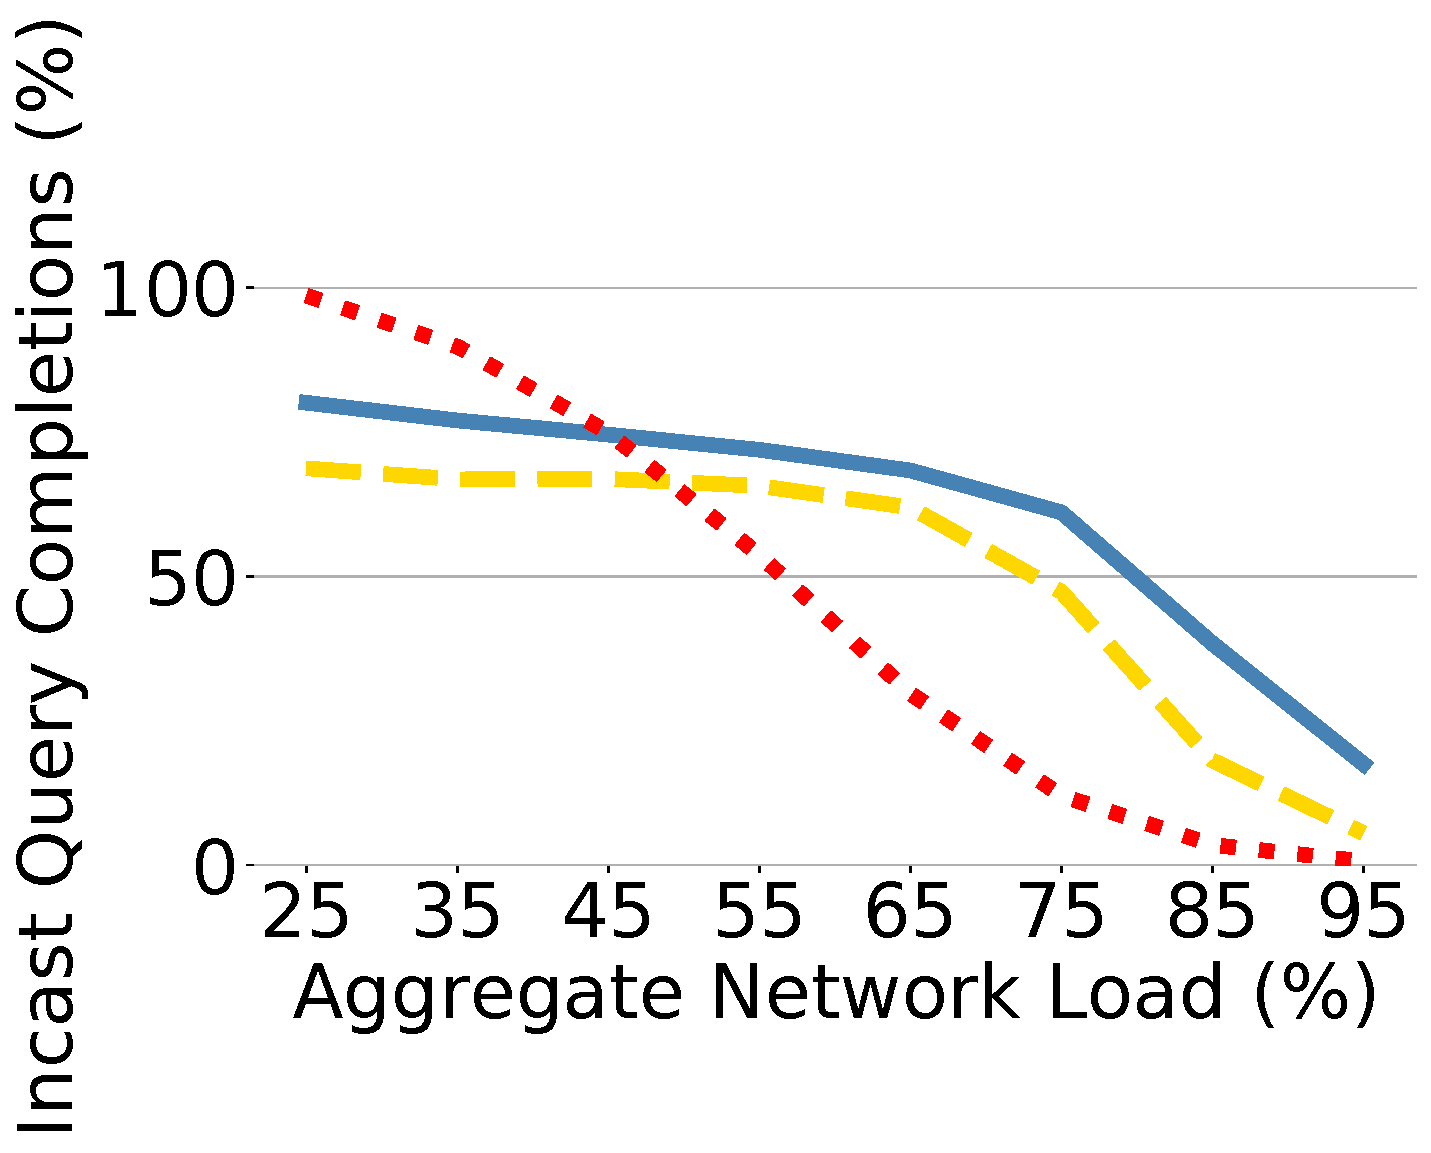
\includegraphics[width=0.98\linewidth]{figs/cc1.pdf}
		\caption{\small{Completion \%}}
		\label{fig:motiv3}
	\end{subfigure}
	\begin{subfigure}[t]{.32\linewidth}
	\centering
	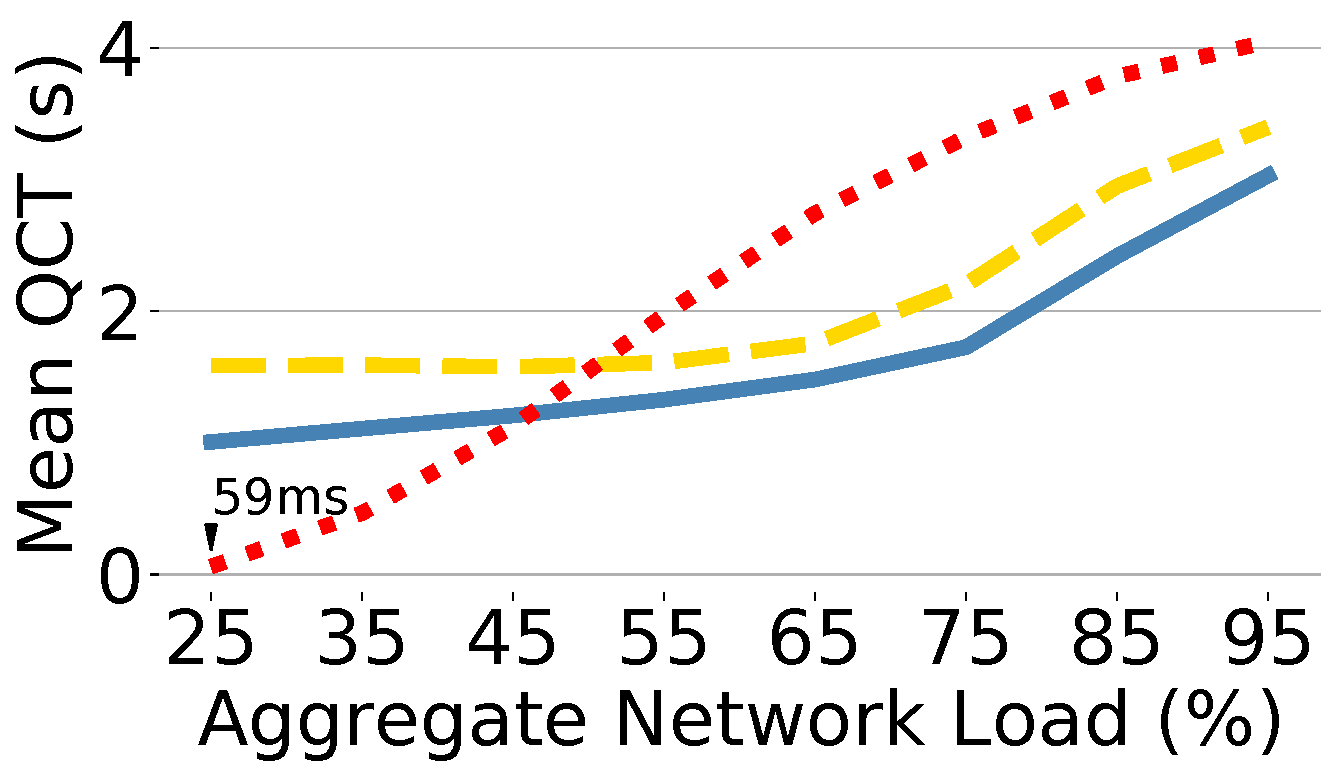
\includegraphics[width=0.98\linewidth]{figs/cc2.pdf}
		\caption{\small{QCT}}
		\label{fig:motiv4}
	\end{subfigure}
		\begin{subfigure}[t]{.32\linewidth}
	\centering
	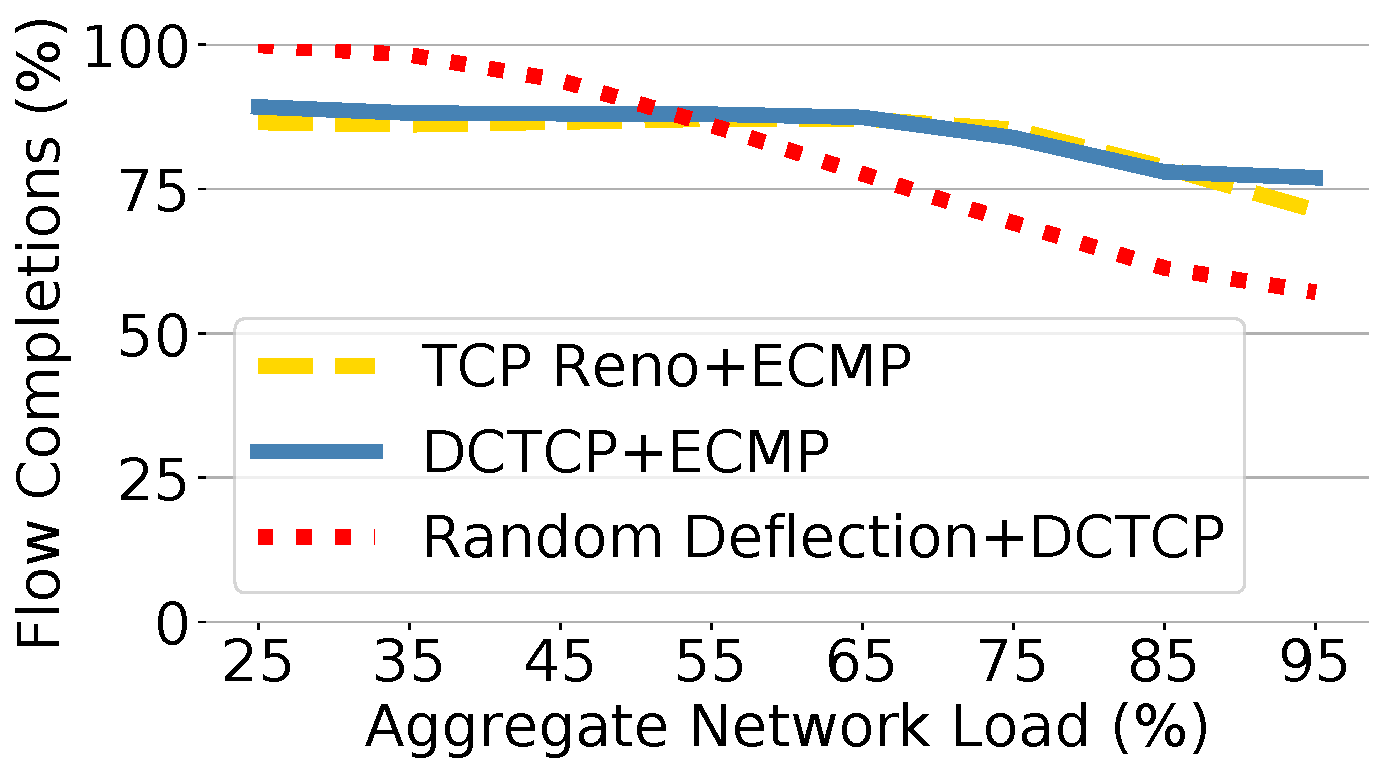
\includegraphics[width=0.98\linewidth]{figs/cc4.pdf}
		\caption{\small{Flow completions}}
		\label{fig:motiv6}
	\end{subfigure}
		\begin{subfigure}[t]{.32\linewidth}
	\centering
	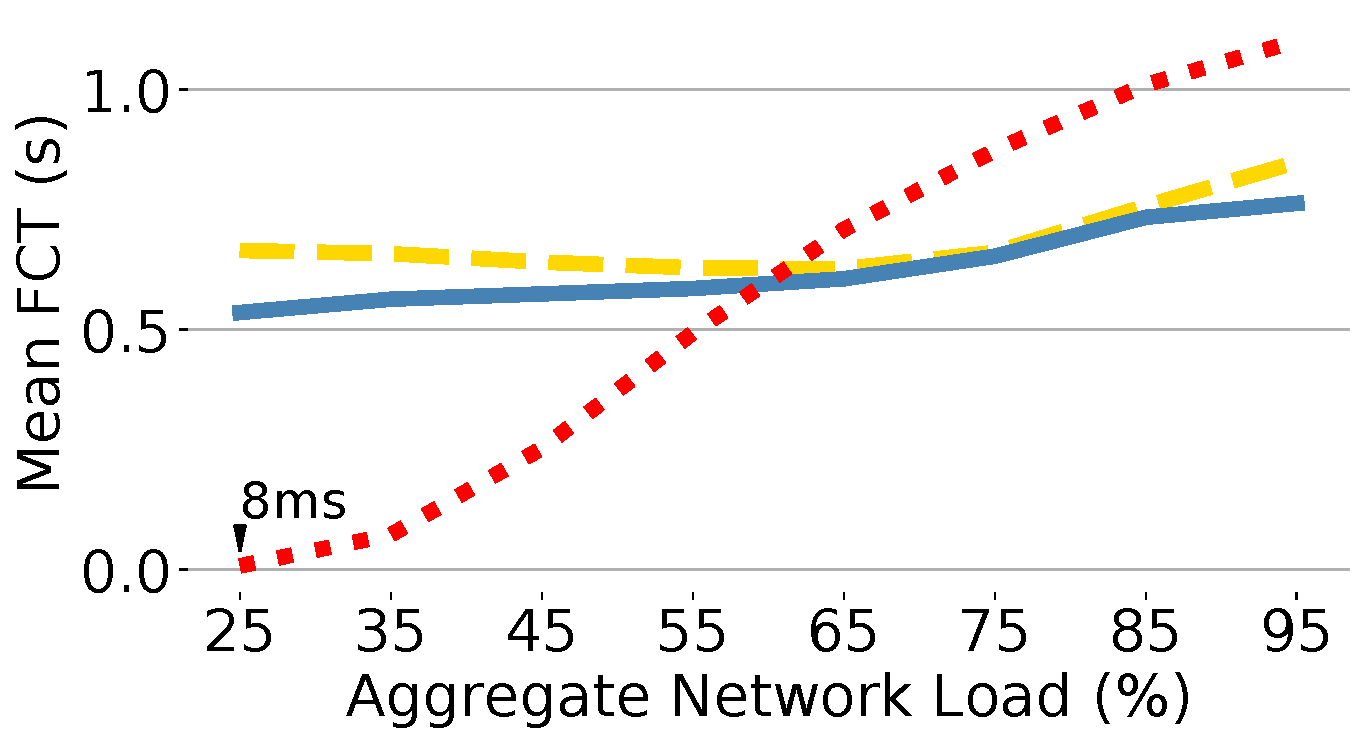
\includegraphics[width=0.98\linewidth]{figs/cc5.pdf}
		\caption{\small{FCT}}
		\label{fig:motiv7}
	\end{subfigure}
		\begin{subfigure}[t]{.32\linewidth}
	\centering
	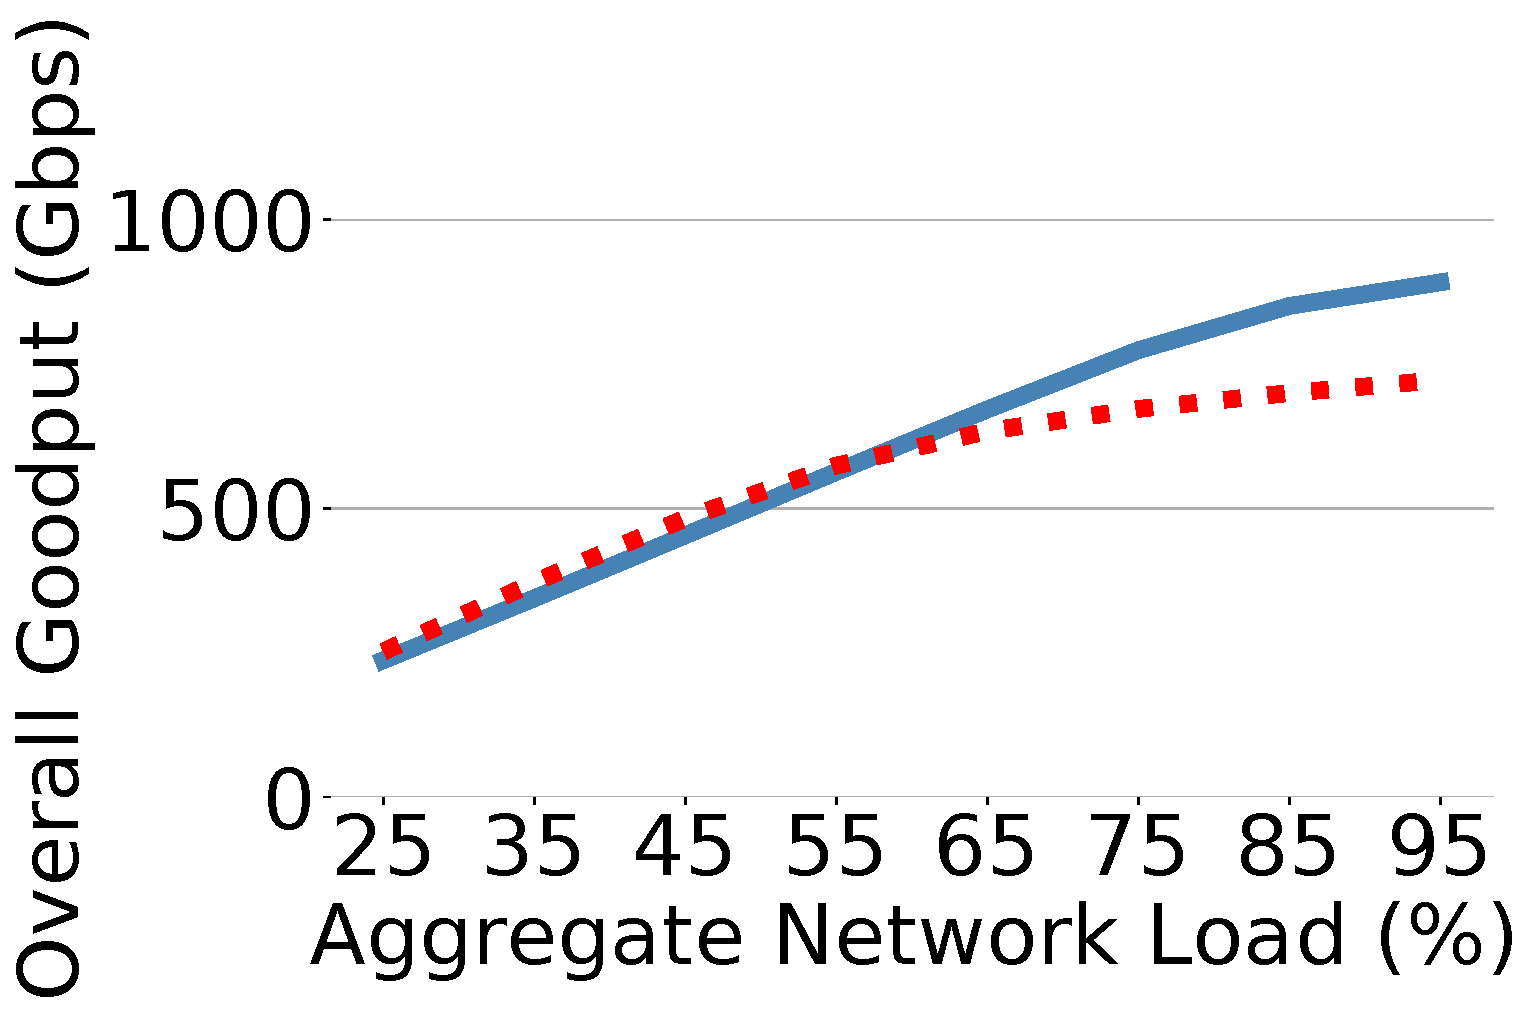
\includegraphics[width=0.98\linewidth]{figs/cc3.pdf}
		\caption{\small{Overall Goodput}}
		\label{fig:motiv5}
	\end{subfigure}
		\begin{subfigure}[t]{.32\linewidth}
	\centering
	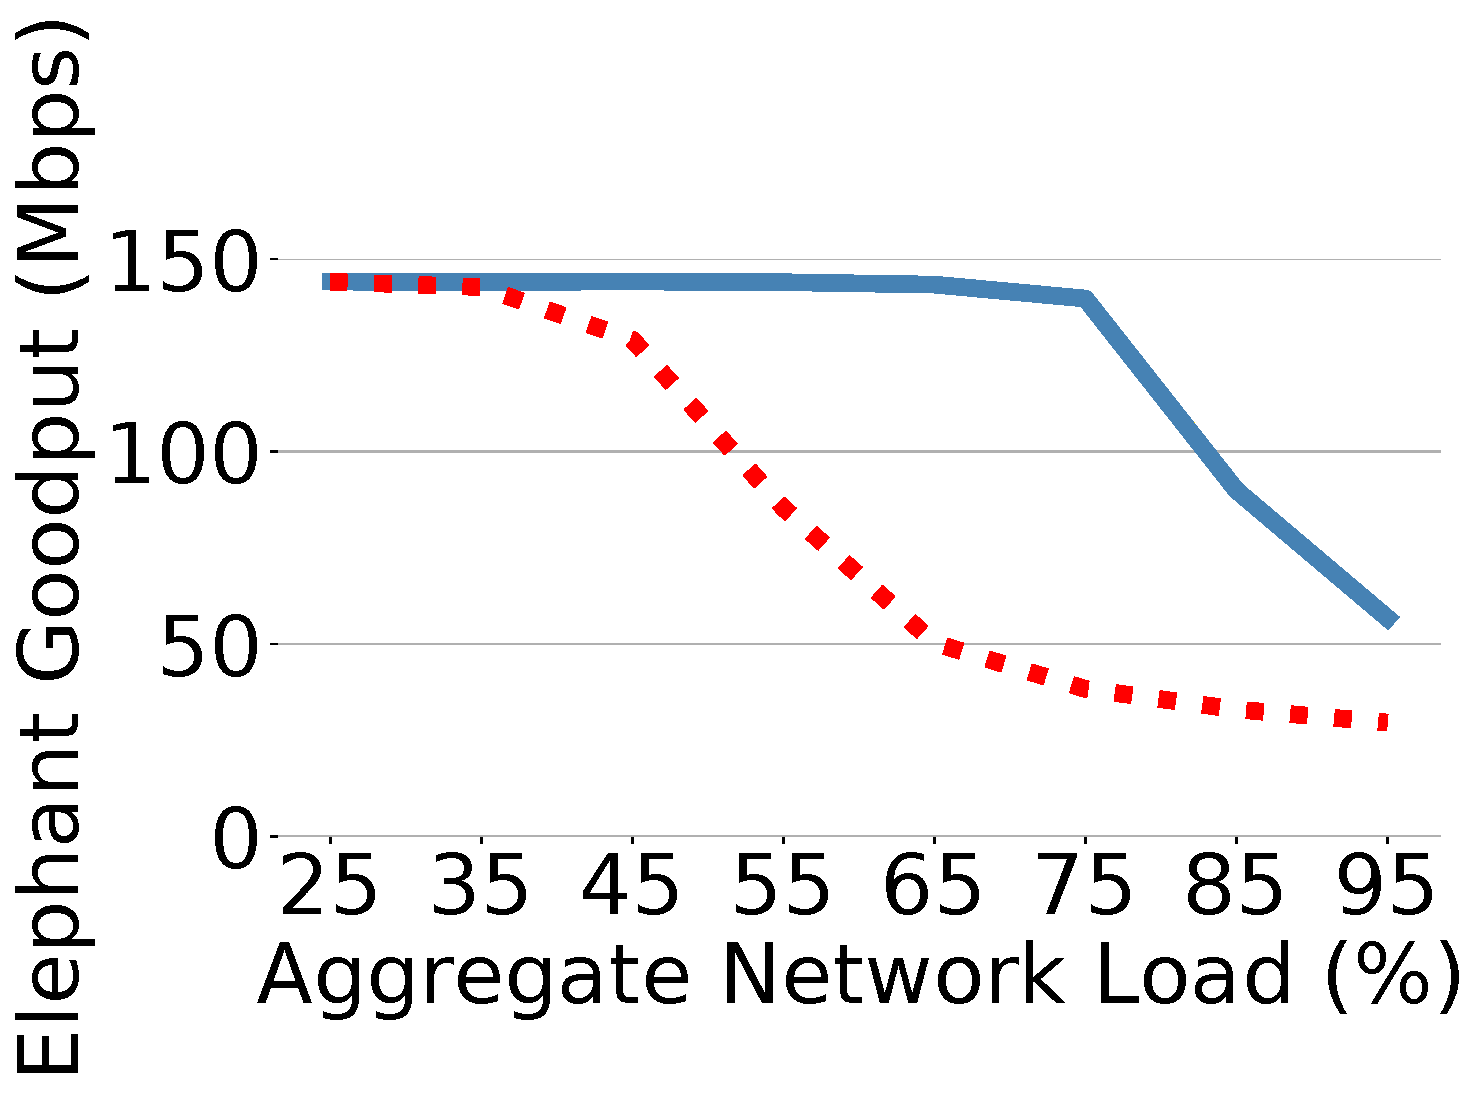
\includegraphics[width=0.98\linewidth]{figs/cc6.pdf}
		\caption{\small{Elephant flow Goodput}}
		\label{fig:motiv8}
	\end{subfigure}
	\caption{\small{Random packet deflection starts to break as the aggregate network load passes 65\% due to excessive RTOs caused by packet drops. The workload consists of 15\% background traffic and varying incast query arrivals.}}
	\label{fig:congestion_collapse}
	\vspace{-2mm}
\end{figure}



To quantify the problem, we simulate a leaf-spine network with 4 cores, 8 aggregates, and a total of 320 servers connected via 10Gbps links to ToR switches with 300KB per-port buffer capacity. We deploy TCP Reno, DCTCP, and DIBS, and write an incast application in which a set of randomly selected clients periodically send queries to 100 randomly selected servers at predefined intervals. Upon receiving a query, each server responds with 40KB of data, and the initiator marks the query as completed after all 100 replies are received. We gradually increase the overall offered load by lowering incast event inter-arrivals in a network filled with 15\% background load (the flow sizes and interarrival times for the background load are from \cite{social}). 
Applying random packet deflection as proposed in DIBS increases the average number of hops that packets traverse by 20\%. As Figure \ref{fig:congestion_collapse} shows, under 80\% load, this results in 54\% \emph{higher} mean query completion times and 30\% \emph{higher} flow completion time tail at 99$^{th}$ percentile compared to ECMP+DCTCP. The results also show that the back-off behavior by random deflection starts to manifest as the aggregate load passes 65\%. After this point, increasing the load results in only a negligible improvement in the application goodput with random deflection (Figure \ref{fig:motiv5}), and a substantial drop in the goodput for elephant flows (flows larger than 10MB) as depictd in Figure \ref{fig:motiv8}.
\emph{These results highlight the need for a smart, load-adaptive deflection technique.}

\textbf{Deflection leads to large delays in completing mice flows.}
Preventing packet drops allows the transmission windows of large flows to grow. Large flows contribute to long-lasting congestion in switch buffers, and their bursty behavior may result in head-of-the-line blocking for short flows. Plus, the amortized added delay of taking longer routes is higher for mice flows.
%a small flow might experience up to 40\% jump in its flow completion time (FCT) under random deflection. 
Our simulations show that random deflection increases the average queueing time of mice flows (< 100KB) by 111\% and increases their average flow completion time (FCT)
by 40\%.
%
\emph{These results suggest that longer flows should be prioritized for deflection.}


\textbf{Deflection results in excessive packet reordering.} 
% \sepehr{Deflecting packets can increase the degree of reordering imposed by the network's core.}
Reordering can reduce throughput and increase flow completion times. 
%Re-ordering is a natural side-effect of packet deflection and needs to be resolved to ensure marginal throughput and FCTs. 
In most TCP variants (including DCTCP), for example, three consecutive duplicate ACKs (resulted from out-of-order delivery) triggers the fast retransmit mechanism where the transmission window is divided in half. To prevent this, some prior techniques, including DIBS, disable the fast retransmit phase \cite{dibs, pabo}. However, when the switch has to drop a packet, perforce (\eg in extreme-scale incasts or in globally congested networks), disabling fast retransmit increases the delay as every dropped packet will require a retransmission timeout (RTO) to be retransmitted. This is generally much slower than the fast retransmit. Our simulation results demonstrate that random deflection increases the packet re-ordering by a factor of 3, leading to 18\% reduction in the overall throughput of large flows under 95\% load.
Plus, network monitoring and diagnosis systems interpret retransmissions and reorderings as signals of network failure \cite{007,blame,netseer}.
\emph{These results underscore the necessity of re-sequencing the packets immediately after they arrive at the destination.} 

\textbf{Deflection causes numerous packet drops even in lightly loaded networks.} 
Deflecting packets to a randomly selected neighboring switch may create congestion in that switch. We verify this by comparing random deflection vs. a load balancing technique inspired by the ``power of two choices'' paradigm \cite{poweroftwosurvey} where for deflecting each packet, we randomly sample two queues and send the packet to the one with lower queue occupancy. In a lightly loaded network with 35\% overall link utilization, random deflection results in 54.5\% higher packet loss compared to the power of two choices technique.
\emph{These results point to an opportunity for 
% better 
balancing the deflected packets evenly in the network.}


We next discuss how we overcame the hurdles of random deflection to build an efficient deflection technique.% that can handle microbursts in datacenters even under extreme levels of load.

\section{Vertigo: Timely Reaction to Microbursts}

\label{sec:v2}

\begin{figure*}[t]
	\centering
	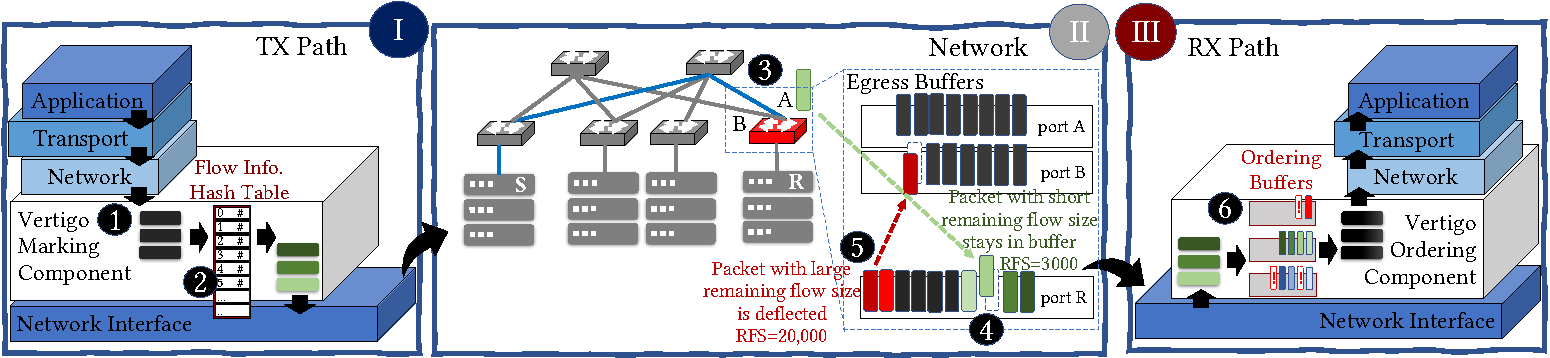
\includegraphics[width=0.99\textwidth]{figs/design-crop.pdf}
	\caption{\small{An illustration of a scenario where a microburst causes the last-hop buffer to overflow. Vertigo absorbs the burst by selectively deflecting packets belonging to flows that contribute to long-lasting congestion.} }
	\label{fig:v2}
\end{figure*}

We present the design of Vertigo, a fast and simple solution to microbursts based on packet deflection. Vertigo is composed of extensions to the host network stack and an in-network deflection and scheduling component. In Vertigo, the sender host marks the outgoing packets with the remaining bytes of the flow. In the network core, Vertigo switches harness this information to selectively deflect packets more likely to contribute to long-lasting congestion when microbursts occur (or to prioritize dropping these packets when the overall load is high). Finally, Vertigo's ordering component, deployed on the receive path at end-hosts, ensures that packets arrive at the transport and higher layers in the correct order that they have been sent. % without relying on the upper-layer header information.

\textbf{An Illustrative example.} Figure \ref{fig:v2} presents an operational overview of Vertigo when the Top-of-Rack (ToR) switch buffer facing the destination host has no room to accommodate the incoming packets.\footnote{This is the most common case of packet drops in datacenters; most of the packet loss (\eg 90\% in a Facebook datacenter \cite{high-resolution}) occur in the ToR-server direction \cite{jupiter, high-resolution}.} The marking component on the TX path, deployed as an independent extension to the existing network stack, receives the packets from the upper layers \blackcircled{1} and marks them with the Remaining Size of the Flow (\emph{RFS}) in bytes (\eg for the last packet of a flow, RFS is equal to packet's payload length)  \blackcircled{2}. 
%This information will enable Vertigo's in-network component to make accurate deflection, dropping, and scheduling decisions based on the provably optimal Shortest Remaining Processing Time (SRPT) paradigm \cite{pfabric, essential} by implementing priority-based buffering primitives in the network core (\S\ref{sec:prio}).
This information will enable Vertigo's in-network component to make accurate deflection, dropping, and scheduling decisions based on the Shortest Remaining Processing Time (SRPT) paradigm \cite{pfabric} by implementing priority-based buffering primitives in the network core (\S\ref{sec:prio}). Even though scheduling flows based on their remaining processing times does not guarantee optimal performance, it is shown to produce near-optimal results when deployed in conjunction with commonly-used congestion control techniques such as TCP or DCTCP \cite{essential,pfabric}. Our results in \S\ref{sec:component} illustrate that Vertigo's use of SRPT paradigm improves the average query completion time by 75\% under 95\% load.
In the network, each switch places the packet in a priority output queue, sorted in ascending order of RFS. That is, packets of the flows with lower remaining sizes will be transmitted first. The packet is forwarded through the network until it reaches a full buffer (the destination ToR in this example) \blackcircled{3}. Inserting the packet in a full priority queue results in buffer overflow and the packet with the largest RFS being dequeued\footnote{In practice, more than one packet may be removed from the queue because of different packet sizes. For simplicity, in this illustrative example, we assume that all packets are identically sized.}. In this example, this results in the green packet (RFS=3000) being enqueued \blackcircled{4} and the red packet (RFS=20000) being popped
% We augment the switch data plane with a buffer design that supports selective deflection. The switch reads the remaining flow size from the packet header and, when the destination buffer is full, finds a candidate packet for bouncing into a neighboring switch to make room for the recently arrived packet with a smaller remaining flow size
 (\S\ref{sec:vertigo}). The dequeued packet is a candidate for deflection: the switch randomly selects two output ports and enqueues the packet to the least loaded one \blackcircled{5}.\footnote{If both queues are full, we randomly select one and insert the deflected packet. This will result in a packet loss but full queues in both the forward and deflection paths signal severe congestion in the network. Therefore, Vertigo does not prevent packet drops in this case.}
%The newly received packet, therefore, replaces the deflected packet inside the buffer \blackcircled{5}. 
Finally, at the destination host, the same RFS field helps Vertigo's ordering component to detect and re-shuffle the out-of-order packets before passing them to upper layers \blackcircled{6} (\S\ref{sec:ordering}).

%Placing the marking component at the edge removes computational and storage overheads from in-network designs that struggle to achieve line-rate throughput when facing complex scheduling decisions or monitoring events \cite{beaucoup, netseer}.
%% I could recall these two papers that talk about the challenge of performing complex processing inside the data plane. Are there any more papers here to add?
% Soudeh: I replaced the "more accurate" part with "a simple and efficient way." We have not evaluated the accuracy of different microburst detection techniques. Plus, our own technique is just a proxy that does have error, e.g., a packet with a large RFS can very well be a microburst packet.
The visibility provided by the sender's network stack allows for a simple and efficient way to distinguish between persistent congestion and \bursts \ without imposing the computational and storage overhead of doing so to the network core, all while enabling transport-independent packet ordering at the destination.
Following the path of a fresh packet, we describe each component in more detail.

\begin{figure}[t]
	\centering
	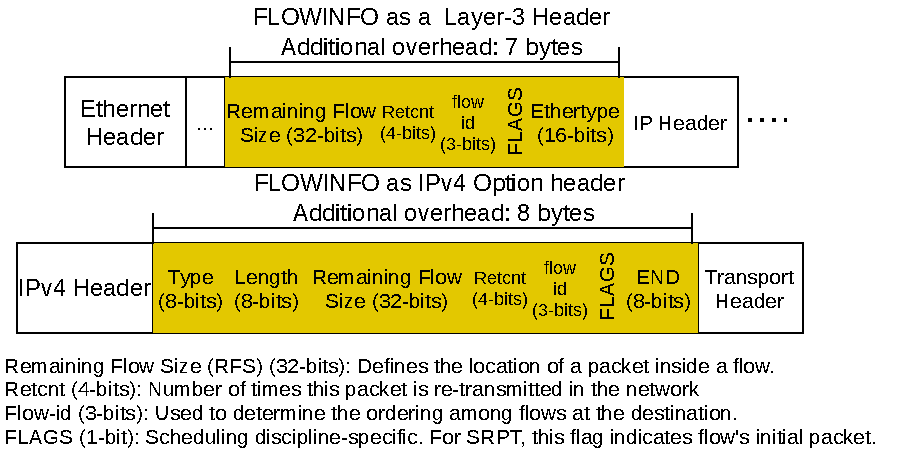
\includegraphics[width=0.75\textwidth]{figs/flowinfo_compact.pdf}
	\caption{\small{Two implementations of the flowinfo header. On top, the flowinfo header is implemented as a layer-3 header that encapsulates the IP header. On the bottom, the flowinfo is implemented inside IPv4 options header.}}
	\label{fig:flowinfo}
		\vspace{-2mm}

\end{figure}

\subsection{TX Path: Marking Component}
\label{sec:prio}

\subsubsection{Priority Framework}

Advance knowledge of flow sizes allows the datacenter network designers to implement scheduling policies that resemble the shortest remaining processing time (SRPT) discipline and therefore achieve near-optimal flow completion times \cite{pfabric, pase, essential, plausible}.
%% The "essential" paper claims that with SRPT scheduling, achieving near-optimal performance is easy.
%% "pfabric" and "pase" are among the earliest works that have implemented SRPT scheduling by explicitly getting the flow size information from the application.
Additionally, storing the remaining flow size inside the packets helps our deflection component avoid deflecting and dropping packets of small flows that are more vulnerable to longer round trip times.\footnote{We also evaluate Vertigo's performance while using flow-aging to mark the packets ($\S \ref{sec:component}$). Vertigo achieves 30\% higher mean QCT under 90\% load while applying flow-aging discipline instead of SRPT.}
To realize SRPT marking, Vertigo receives flow size information from the application and keeps track of the remaining bytes of outgoing flows inside a hash table. Vertigo tags each packet with the remaining bytes of its flow.

% It's worth noting that Vertigo can promptly adapt other aging policies with minor modifications to the header format and marking procedures. We present the performance achieved by replacing SRPT with Least Attained Service (LAS) counters in \S\ref{sec:eval}. The readers can find an operational overview of V2 under LAS scheduling and strict priorities in Appendix \ref{sec:alternative}.

Figure \ref{fig:flowinfo} depicts two potential implementations for Vertigo's auxiliary \textit{flowinfo} header.
A 32-bit field shows the flow's remaining bytes. Its uniqueness across packets of a single flow allows the ordering component to detect and resolve packet re-ordering. 
Additionally, we add a 4-bit counter, \textit{retcnt}, to track the number of re-transmissions each packet has experienced, a 3-bit counter, \textit{Flow-id}, to ensure correct ordering between subsequent flows, and a single-bit flag to mark the first packet of the flow (\S\ref{sec:ret}).

\subsubsection{Detecting duplicate packets.}
\label{sec:ret}
% To further support re-transmissions and avoid sending the same packet with multiple sequence numbers, Vertigo calculates a CRC hash from the first 64 bytes of every packet and stores it in a per-flow hash table. The rationale behind this hashing is to detect duplicate packets by scanning the protocol headers. Upon detecting a re-transmission, Vertigo tags the packet with its original sequence number and sets \textit{retcnt} in the auxiliary header to match the number of re-transmissions that it has experienced thus far.

% If the hash lookup fails,--meaning that this is likely the first transmission-- a unique sequence number is added to the packet hash table along with its hash value as the key. 
% \soudeh{Does this mean that the sender host has to store a (key,value) pair for every single packet?}
% 's ordering component  will use the sequence numbers to detect out-of-order arrival of packets.
% Figure \ref{fig:design} presents the high-level design of Vertigo. The marking component is placed near the link layer in the tx path and keeps track of flow sequence numbers and packet hash tables.
Packet loss and re-transmissions are inevitable in lossy networks. To ensure that the \textit{flowinfo} header information remains consistent, the marking component must detect duplicate packets and retrieve their original RFS field.
Moreover, persistently deflecting or dropping packets of large flows may eventually lead to their starvation. 
% To prevent this, Vertigo boosts the priority of re-transmitted packets by reducing their RFS values.
To prevent this, Vertigo employs a \textit{boosting mechanism} as part of the marking component in which the priority of re-transmitted packets is elevated by reducing their RFS values. Concretely, every time a packet is re-transmitted, Vertigo divides its RFS by a user-defined \textit{boosting factor}. In our evaluations, unless stated otherwise, we set the boosting factor to 2.
The boosting procedure
% This
diminishes the risk of starvation and repeated re-transmission timeouts, even for packets of large flows. 
%that contribute to long-lasting congestion.

Vertigo's marking component detects re-transmissions by calculating a CRC hash of packet headers and looking it up in a cuckoo filter \cite{cuckoo} to enable fast look-up and updates in the dataplane. It then applies the boosting function to the original RFS field of the packet stored in the flow 
table and increments the \textit{retcnt} field in the \textit{flowinfo} header. This operation needs to be reversible at the receiver to maintain the synchrony between the sending and receiving components; therefore, we confine the marking component to perform only bitwise rotations on the RFS field. Doing so relieves the network components from performing any computations on \textit{flowinfo} header fields and allows the destination to apply an inverse boosting function and retrieve the original RFS of the packet.
% \sepehr{ which means that the value of the boosting factor is always a power of 2}.
This limitation implies that the boosting factors must be chosen from powers of two, yet we show that even 2$\times$ boosting is enough to properly mitigate starvation.


% The RFS for a re-transmitted packet $P$, denoted by $P_{RFS}$, is updated by performing a user-defined ($m$) bitwise right rotations on the original RFS ($P_{OldRFS}$):
% \begin{equation}
% P_{RFS} = \frac{1}{2^m} P_{OldRFS}
% \end{equation}

% \sepehr{The RFS for a re-transmitted packet is updated by performing a user-defined ($m$) bitwise right rotations on the original RFS ($P_{OldRFS}$):
% \begin{equation}
% P_{RFS} = \frac{1}{2^m} P_{OldRFS}
% \end{equation}}

With the boosting factor of 2, Vertigo sets the RFS for a re-transmitted packet to half of its previous value by performing a bitwise right rotation on the original RFS. 
%Concretely, the RFS of a re-transmitted packet is set to half of its previous RFS value, 
This reduces the probability of it being selected again for deflection or dropping in the network.
At the destination, Vertigo performs bitwise left rotations on the packet to retrieve the packet's original RFS. Using a 32-bit RFS field, Vertigo can support up to 16 re-transmissions for every packet. In \S\ref{sec:component}, we  evaluate the impact of boosting function on Vertigo's performance and illustrate that, while boosting can increase the percentage of completed queries by up to 60\%, increasing the boosting factor has negligible impact on overall performance.
%re-transmissions on flow completion times.

% \fixme{\textbf{[COVERED]} Add more details on how we do boosting. Add the details about its parameterization.}
% \fixme{It will be better if we simplify the design to not have parameters and ``user-defined'' parts. I think we can just remove `m' all together, except for a brief discussion in the evaluation discussing that different values of it do not lead to any notable diff in the results.}

% Finally, we note that storing the flow status in the data plane is relatively straightforward. Vertigo detects flows using 5-tuple CRC hash functions and stores flow RFS as data pointers inside a hash table. Vertigo also uses pre-allocated cuckoo filters \cite{cuckoo} to store a CRC checksum of packet headers, thus performing two fast hash table lookups per each packet. In our testbed evaluation of Vertigo, we show that the marking overheads on aggregate throughput and latency are negligible (\S\ref{sec:testbed}).

\subsection{Selective Deflection in the Network}
\label{sec:vertigo}
% Vertigo's design insight is to overcome the challenges of packet deflection by imposing the deflection delay, \ie the delay imposed by deflecting or dropping a packet under extreme congestion, to the packets of the flows that are likely to contribute to long-lasting congestion. To this purpose, Vertigo exploits per-packet forwarding and deflection. \sepehr{we might be able to remove this paragraph}
We assume that switches use output queues sorted by packet ranks, where \emph{ranks} are the RFS fields provided by Vertigo's marking component.\footnote{Recent works provide practical implementations of this abstraction \cite{pifo, pieo}. 
%In \S\ref{sec:testbed}, we briefly describe our proposed extensions to these designs.
} We also assume that switch forwarding tables are pre-populated with the information of the next-hops for every destination. 
%Furthermore, considering the recent advances in implementing priority queues at line rate \cite{pifo, pieo, calendar} and Vertigo's use of priority queues to implement SRPT scheduling and selectively detour and drop packets, we assume that all output queues are priority queues.
%
%Packets departing from end-hosts arrive at the switches with an auxiliary header that contains the remaining bytes of the flow they belong to (RFS). 
Inspired by the 
``power of two choices''
paradigm \cite{poweroftwosurvey}, when a switch receives a packet that has more than one possible next hop, the switch compares the queue lengths of two random ports and sends the packet to the least loaded one. 
% \Erfan{Power of two choices forwarding has two main benefits. First, it allows for fine-grained traffic distribution, hence, aiming for higher throughput guarantees. Second, it prevents the synchronization effect of multiple forwarding engines choosing the least loaded port simultaneously \cite{drill}.} 
In addition to the simplicity of its hardware implementation, the power-of-two choices forwarding enables fine-grained traffic distribution, hence, delivering higher throughput guarantees.  
%Second, it prevents the \textit{synchronization effect} caused by choosing from more randomly selected ports (more generally referred to as power-of-n choices) \cite{drill}. Particularly, with the power-of-n choices scheme, selecting the least loaded port among more options creates the chance for a single port to be simultaneously chosen by multiple source ports. The power-of-two choices paradigm avoids this problem by exploiting randomness.}
% \sepehr{(I iterated over the parts where we mention power-of-two choices in the paper. I believe we provide both the definition and the intuition (better balancing the load) throughout the paper. I only added drill as another citation for power-of-two choices.)}
To apply SRPT scheduling, Vertigo sorts packets in each queue in increasing order of their RFS fields. When the link is idle and there are packets stored in the output queue, Vertigo transmits the packet with the smallest RFS, \ie the packet stored at the head of the queue.


To manage \bursts, Vertigo tries to exploit the networks' extra capacity to absorb \bursts.
%\ by preventing packet drops while imposing the deflection delay, \ie the delay imposed by deflecting or dropping a packet under extreme congestion, to packets of flows that are more likely to contribute to lasting congestion: those with more remaining packets to transmit. 
Concretely, when a switch receives a packet and its output queue is full, the switch selects the packet with larger RFS between this packet and the tail of its queue to deflect. For deflecting a packet, the switch randomly selects two queues and enqueues the packet into the least loaded one. If both queues are full, the switch enqueues the packet in one of them (randomly selected). This will result in one or more packets being dropped from the tail of this queue. 

For both forwarding and deflecting packets, Vertigo uses the 
% ``power of two choices'' 
power-of-two choices 
paradigm to evenly distribute the load across the network. However, in contrast to forwarding (where a full queue results in \emph{deflecting} packets), Vertigo \emph{drops} packets if it encounters full buffers when it tries to deflect a packet. This distinction is intentional.
While encountering a full buffer on the forward path can be a result of a local, short-lived microburst \ (\eg at the destination ToR in incast) and not necessarily an overall congested network, the output queue and two randomly selected ones all being full at the same time is a strong indication of extensive, extreme congestion. Via dropping packets in the latter case, Vertigo triggers the congestion control algorithms to throttle the send rates.
%
Overall, Vertigo prioritizes packets of flows that are more likely to contribute to lasting congestion, \ie those with more remaining packets to transmit, for deflection and dropping. This helps Vertigo absorb \bursts \ even when the network is congested.

% The fact that you use different techniques for forwarding and deflection is one of the means of treating long-lasting congestion and microbursts differently, I suppose. E.g., compared to congestion in the forward path (e.g., at the last hop for inacst), congestion for a deflected packet (i.e., two randomly selected queues both being full) more likely shows that the network is overall congested. The text does not discuss this. It should. It's an important part.
%
% While less likely, it is still probable that both randomly chosen destination buffers are full. In this case, Vertigo treats the deflected packet as a newly arrived packet to either of the two buffers and repeats the deflection process, only this time dropping the packet with highest RFS. This is another opportunity for Vertigo to treat long-lasting and microburst flows differently since the drop decision selectively targets a flow with the most remaining bytes. This is important because bumping into full buffer twice is a good indicator of severe congestion, and we want persistent flows to back-off quickly until the congestion event is resolved.

% For Vertigo to perform well, two main challenges must be addressed:

% \begin{enumerate}
%     \item \textbf{Starvation of large flows:} Applying per-packet SRPT scheduling at the switches might result in the starvation of large flows \cite{pfabric}. Vertigo avoids starvation by decreasing the RFS of packets each time they are retransmitted (\S\ref{sec:prio}).
    
%     \item \textbf{Excessive reordering:} Both deflection and per-packet SRPT scheduling impose excessive reordering and hurt throughput. To avoid this, Vertigo implements a transport-independent ordering layer at the receiver hosts’ networking stack to absorb the reordering caused by deflection and scheduling (\S\ref{sec:ordering}).
% \end{enumerate}

% By moving the starvation prevention process to the end hosts, Vertigo's switch design is implementable at line rate using programmable hardware \cite{pifo, pieo}.



\subsection{RX Path: The Ordering Component}
\label{sec:ordering}

The ordering component on the receive-side is the first software entity that obtains packets from the NIC. Its task is to detect out-of-order packets and temporarily buffer them until the delayed segments arrive or are timed out. To this end, Vertigo first extracts the \textit{flowinfo} header. For every active flow, Vertigo stores the expected RFS and two intermediate linked lists containing references to the ready and out-of-order packets, respectively. RFS fields inside the \textit{flowinfo} header are unique among the packets of a flow except for the re-transmitted packets. Since the re-transmission boosting mechanism may modify the RFS field (see \S\ref{sec:ret}), Vertigo first reverts the boosted RFS by applying \textit{retcnt} left rotations on a packet's RFS field. 
% Equation \ref{eq:reverse} formulates the reverse boosting function where \textit{$P_{RFS}$} is the RFS in the \textit{flowinfo} header and  \textit{$P_{retcnt}$} is the number of re-transmissions the packet has experienced.

% \begin{equation}
% \label{eq:reverse}
%     P_{RFS} (i) = P_{RFS}((i+P_{retcnt}) \mod 32), \forall i \in \{1..32\}
% \end{equation}

\begin{figure}[t]
	\centering
	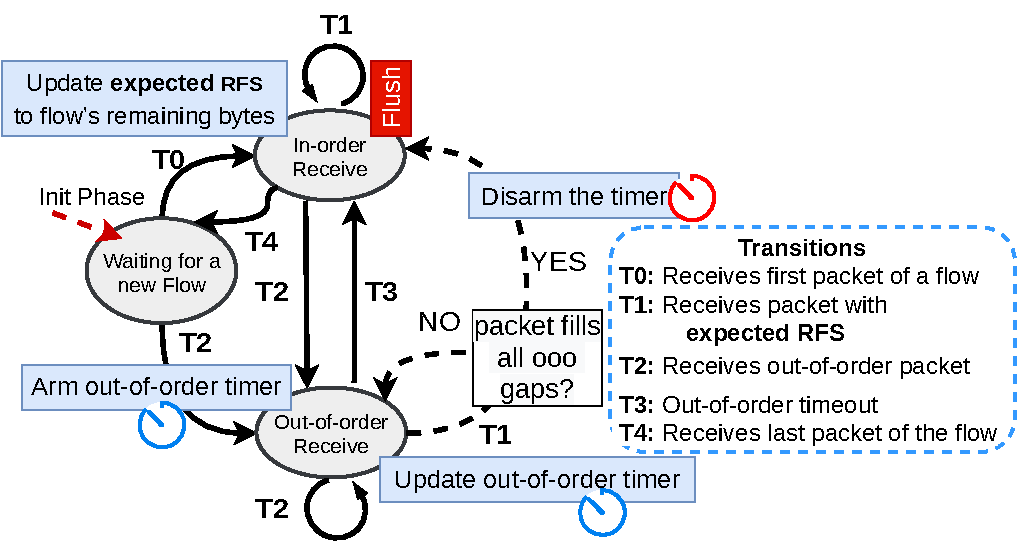
\includegraphics[width=0.75
	\textwidth]{figs/reordering_state_machine.pdf}
	\vspace{-2mm}
	\caption{\small{The state-machine decides the fate of arrived packets. Out-of-order packets are placed inside a separate buffer, arming a timer to wait for delayed packets. In-order packets are immediately flushed to the network stack.}}
	\label{fig:state_machine}
		\vspace{-2mm}
\end{figure}

\subsubsection{Ordered Receive.}
When the destination host receives a packet, it checks the RFS present in the \textit{flowinfo} header. Vertigo expects a packet flagged as the initial packet of a flow to arrive first. Any packet with a larger counter indicates that there has been reordering or drops in the network. Figure \ref{fig:state_machine} presents the state machine of the ordering component. After receiving the first packet of a flow, the state machine transitions to the \textit{In-order Receive} state and continues to receive packets until an out-of-order packet arrives or the flow terminates. While in the \textit{In-order Receive} state, arrived packets are placed in an intermediate buffer, and the protocol stack's receive routines are signaled to begin processing them immediately. The expected RFS is then updated by subtracting the received packet's size from the previously expected RFS value.
However, when an out-of-order packet arrives, the ordering component designates a separate pre-allocated buffer to store early packets and wait temporarily for the in-transit packets. Upon receiving the entire flow, the state machine transitions back to the initial state (\textit{Waiting for a new flow}). This is conceptually similar to the design of \cite{juggler}, except that Vertigo does not rely on GRO buffers or TCP sequence numbers to perform re-shuffling.

\subsubsection{Out-of-order Receive.} When in the \textit{Out-of-order Receive} state, a timer is armed to prevent long pauses in packet processing caused by dropped packets. The waiting time depends on the network topology, link bandwidth, and link utilization. We define the waiting time ($\tau$) as the maximum duration of time that the ordering component waits for a single delayed packet before starting to process out-of-order packets. While a short timeout increases the degree of reordering in the transport layer, large timeouts increase the flow completion tail latency. A safe estimate of $\tau$ is the time it takes for a single packet to traverse a network with almost full buffers. In the topologies we used in our evaluations, we set $\tau = 360\mu s$. \S\ref{sec:component} explores the impact of $\tau$ configuration on flow completion times.

Four events can occur when in \textit{Out-of-order Receive}: 1) The host continues to receive early packets. In this case, the ordering component continues to buffer these packets along with their arrival timestamp until either timeout occurs or the expected packets arrive. 2) The host receives a packet that fills one of the gaps in the ordering buffer. Henceforth, the component can move its expected receive window forward to the next gap in the out-of-order buffer, update the timeout timer by subtracting the elapsed time from the arrival of next out-of-order packet from $\tau$, and place the in-order packets in the \textit{ready} buffer. After filling all the gaps, the state machine transitions back to \textit{In-order Receive} state and disarms the timer. 3) The host receives packets with an RFS that is smaller than the expected RFS. This may indicate the arrival of delayed re-transmissions or a duplicate packet. Vertigo ignores packets that are already inside the ready buffer and places the late packets at the head of the ready buffer to send them up to the transport immediately. 4) The re-ordering timeout occurs. In this case, the re-ordering component releases all packets until the next gap up to the transport layer to trigger the protocol-specific decisions. It moves its expected packet pointer to the next gap in the out-of-order buffer and updates the timer. Finally, unless the out-of-order buffer is not empty, the system transitions to \textit{In-order Receive}.

% \fixme{\textbf{[COVERED]} Talking about the reviewer's concern regarding the intervention of the ordering timer to the protocol's operation. Talk about the difference between our and transport's timeouts.}

% \sepehr{One might argue that Vertigo's ordering component might interfere with transport-layer's loss recovery. Being deployed on the receive-side, the ordering component does not interfere with timers triggered at the sender hosts' networking stack, such as TCP re-transmission timer, but it might interfere with mechanisms like TCP fast-retransmition, by temporarily delaying the subsequent packets of a dropped packet. 
% % Besides being protocol-agnostic, the ordering component aims to absorb the redundant reordering while exploiting the loss recovery procedures of the transport protocol, \ie fast re-transmission and recovery. 
% The power-of-two choices load-balancing and packet deflection cause heavy re-ordering that triggers redundant fast re-transmissions, causing many unnecessary duplicate packets entering the congested network and reducing the overall application throughput. Random deflection solutions, such as DIBS, disable TCP fast re-transmission to prevent the consequences of excessive re-ordering \cite{dibs, pabo}. This causes the packet loss to be detected only by re-transmission timeouts (RTOs), further delaying the loss recovery process. In Vertigo, we configure ordering timeouts to be small enough to still trigger fast-retransmition in the case of packet loss while preventing the injection of unnecessary duplicate packets into the network. This ensures that Vertigo’s interference with existing congestion control mechanisms is minimized.}

Previous proposals on random deflection disable TCP fast re-transmit to prevent the consequences of excessive re-ordering \cite{dibs, pabo}, such as injection of redundant duplicate packets. This causes the packet loss to be detected only by re-transmission timeouts (RTOs), further delaying the loss recovery process. In Vertigo, we configure ordering timeouts to be small enough to still trigger fast re-transmission in the case of packet loss, while preventing the injection of unnecessary duplicate packets into the network. This ensures that Vertigo’s interference with existing congestion control mechanisms is minimized.

% The ordering layer is implemented as the first entity in the networking stack of the receiver host, and its timer does not interfere with the timers used by transport protocols, such as RTO timer, for re-transmitting a packet, as these timers are applied at the sender host.
% However, the reviewers make a valid point about the ordering layer interfering with mechanisms such as TCP fast-retransmit, by holding the subsequent packets of a dropped packet. The power-of-two choices load-balancing and packet deflection result in heavy re-ordering that in-turn triggers redundant fast-retransmissions, causing many unnecessary duplicate packets entering the congested network (and reducing the overall application throughput). Random deflection solutions, such as DIBS and PABO, disable TCP fast re-transmit to prevent the consequences of excessive re-ordering. This causes the packet loss to be detected only by re-transmission timeouts (RTOs), further delaying the loss recovery process.
% In Vertigo, we configure ordering timeouts to be small enough to still trigger fast-retransmit in the case of packet loss while preventing the injection of unnecessary duplicate packets into the network. This ensures that Vertigo’s interference with existing congestion control mechanisms is minimized.
% It is also worthwhile to note that Vertigo tries to be protocol-agnostic; therefore, adding the Vertigo logic to the transport protocol would violate this very design goal.










% flow id settings
% 

% \textbf{Receiving packets from different flows.} In some circumstances, due to improper timeout settings and excessive deflection, a packet might remain in the network for a long enough time that the  is reset in the source and its packets arrive at the destination earlier. With only sequence numbers as the arrangement indicator, the ordering component might identify the new arrivals as stale clones of previously flushed packets and incorrectly place them inside the \textit{ready} buffer. In addition, since the ordering component considers the arrival of packets with a sequence number (0) as the termination of the previous flowlet, if D is set correctly based on the expected delay each packet experiences in the network), the ordering component updates its expected sequence number to wait for new flowlet. If, however, any outstanding packet from previous flowlets with a larger sequence number arrives, the component might incorrectly store them in the \textit{out-of-order} buffer for a long time.

% To avoid such corner cases, Vertigo dedicates four spare bits in the \textit{flowinfo} header to \textit{flowlet-id} counter, and increments it each time a new flowlet starts at the marking component. This gives the receiver the ability to keep track of the current flowlet counter value and detect packets from previous or next flowlets to properly decide their fate. When the receiver expects packets with \textit{flowlet-id}=$m$, receiving packets from flowlet $n, n>m$ result in one of two possible outcomes: 1) If the packet sequence number is 0, the receiver updates its expected flowlet-id and sequence number, flushing all of the buffers for that flow up to the transport. 2) Otherwise, Vertigo buffers the received packet and waits for a packet with sequence number=0, before transitioning its state.


\textbf{Summary: }
% What we wanted to do
We presented the design of Vertigo, a burst-tolerant routing technique for datacenters that deflects excess packets to neighboring switches to absorb \bursts. To prevent the performance degradation of deflection under high load, Vertigo prioritizes deflecting (and dropping, when the network is overloaded) the packets of the flows with more remaining bytes to send as they are more likely to contribute to lasting congestion. Furthermore, it employs a boosting mechanism to further assist with flow completions and prevent starvation. To enable these, we augmented the hosts' network stack with a transport-independent fast packet processing framework that performs packet marking on the TX path and packet ordering on the RX path. 
%We held forth the design of a deflection mechanism inside the switching fabric that is able to selectively forward and deflect packets based on flows' remaining bytes. Finally, we introduced Vertigo's ordering component to mask the re-ordering side-effects of packet deflection. Vertigo's ordering component makes use of the remaining flow size fields inside the packet to determine its correct position and provisionally buffer out-of-order packets. Our holistic approach to react to microbursts dramatically reduces the number of packet drops and expensive re-transmission timeouts caused by bursty traffic.

\section{Performance Evaluation}
\label{sec:eval}


% \begin{figure}[t]
% 	\begin{subfigure}[t]{.49\linewidth}
% 	\centering
% 	\includegraphics[width=0.98\linewidth]{figs/qps50tcpdctcp.pdf}
% 		\caption{Completed Incast Queries}
% 		\label{fig:tcp_qc}
% 	\end{subfigure}
% 	\begin{subfigure}[t]{.49\linewidth}
% 	\centering
% 	\includegraphics[width=0.98\linewidth]{figs/qps50tcpdctcpcdf.pdf}
% 		\caption{Mean QCT}
% 		\label{fig:tcp_qct}
% 	\end{subfigure}
% 	\caption{Vertigo implicitly performs congestion control on large flows. Without congestion notification mechanisms, flows are able to automatically adjust their transmission under Vertigo.}
% 	\label{fig:tcp}
% \end{figure}




% \begin{figure*}[t]
% % 	\begin{subfigure}[t]{.49\linewidth}
% % 	\centering
% % 	\includegraphics[width=0.98\linewidth]{figs/flowsize50qc.pdf}
% % 		\caption{Completed Incast Queries}
% % 		\label{fig:size_qc}
% % 	\end{subfigure}
% 	\begin{subfigure}[t]{.24\linewidth}
% 	\centering
% 	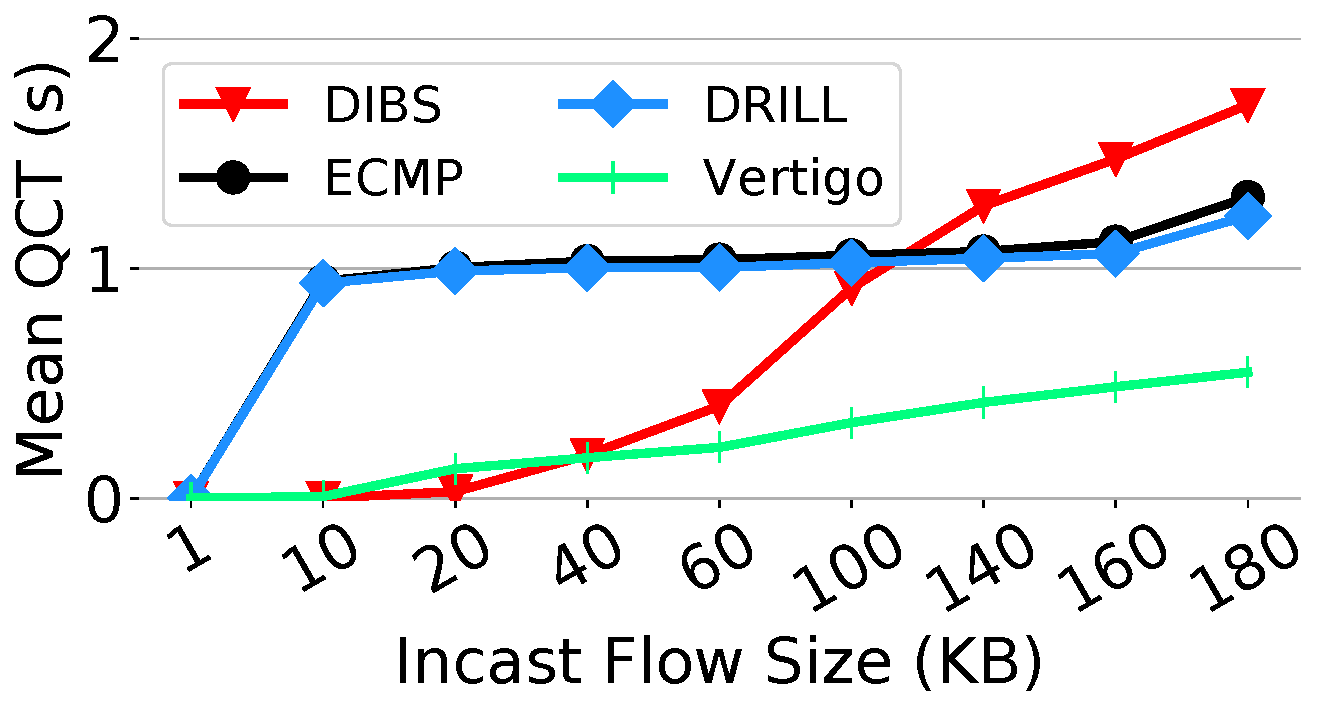
\includegraphics[width=0.98\linewidth]{figs/flowsize50qct.pdf}
% 		\caption{Mean QCT}
% 		\label{fig:size_qct}
% 	\end{subfigure}
% 	\caption{Vertigo maintains a high query completion rate even with large Incast flows.}
% 	\label{fig:size}
% \end{figure*}


% \begin{figure*}[t]
% 	\centering
	
% 	\begin{subfigure}[t]{.20\linewidth}
% 	\centering
% 	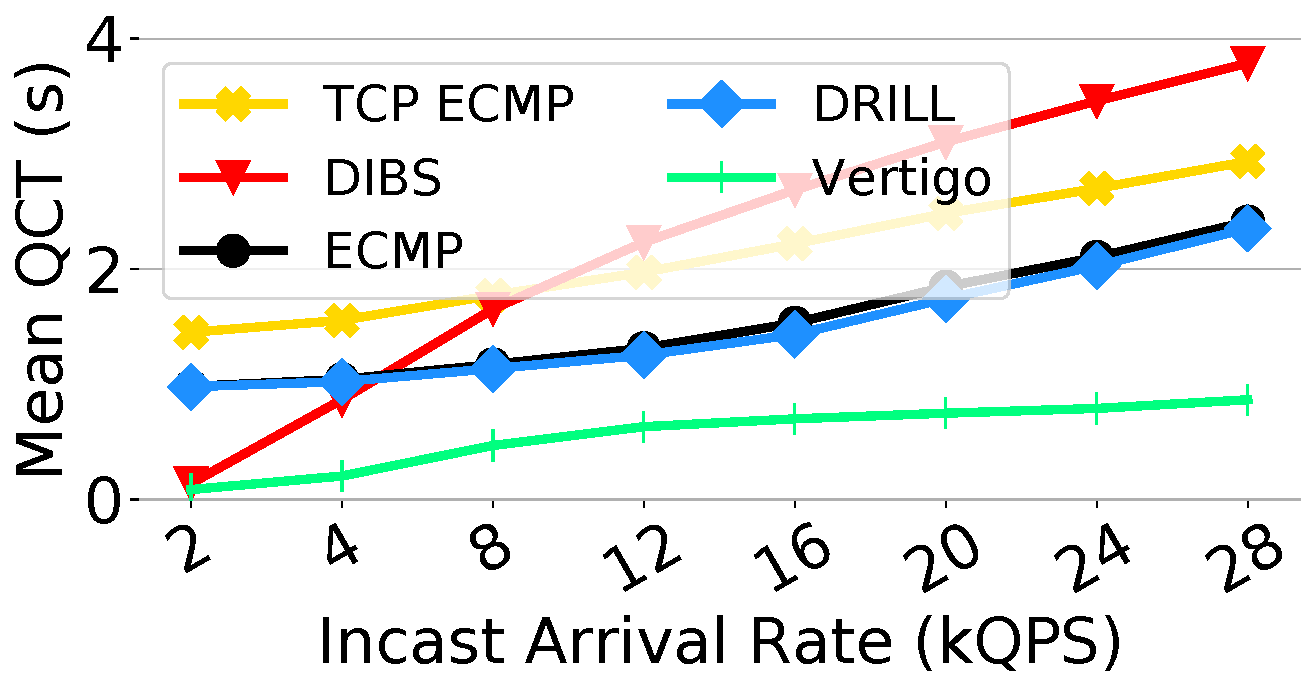
\includegraphics[width=0.98\linewidth]{figs/burst80.pdf}
% 		\caption{ \Erfan{25\% overall load PLACEHOLDER}}
% 		\label{fig:burstiness25}
% 	\end{subfigure}
% 	\begin{subfigure}[t]{.20\linewidth}
% 	\centering
% 	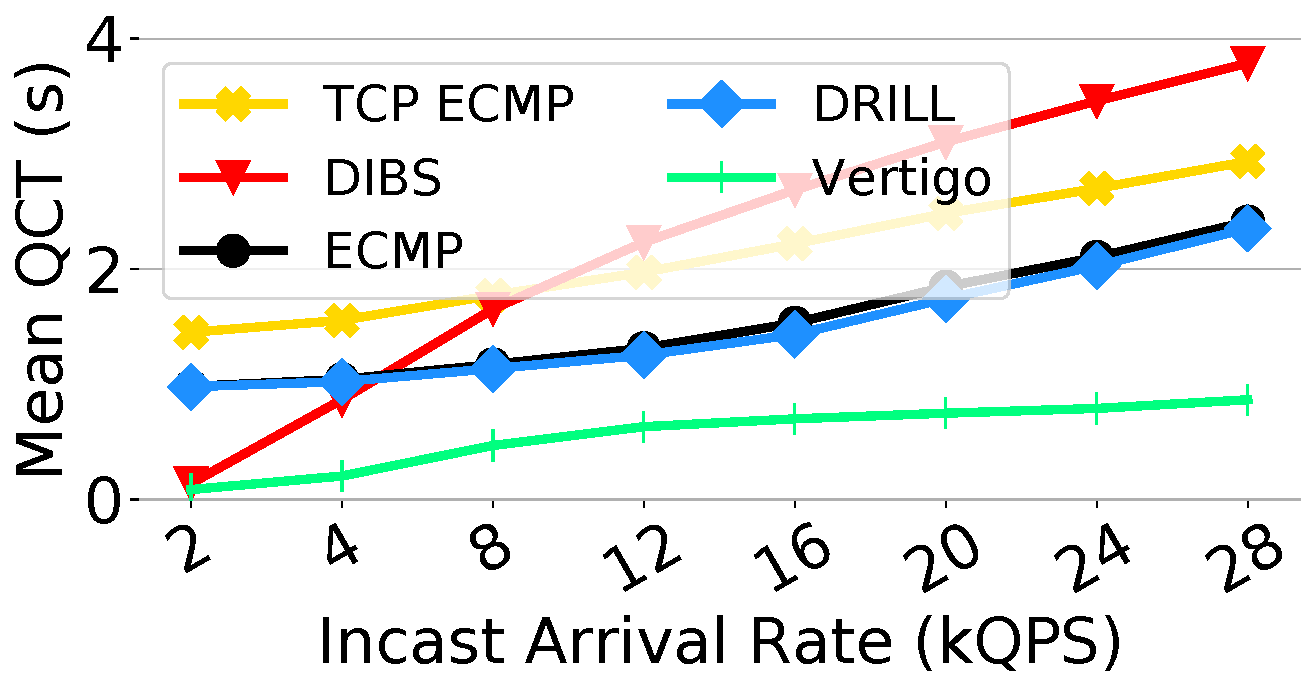
\includegraphics[width=0.98\linewidth]{figs/burst80.pdf}
% 		\caption{\Erfan{50\% overall load PLACEHOLDER}}
% 		\label{fig:burstiness50}
% 	\end{subfigure}
% 	\begin{subfigure}[t]{.20\linewidth}
% 	\centering
% 	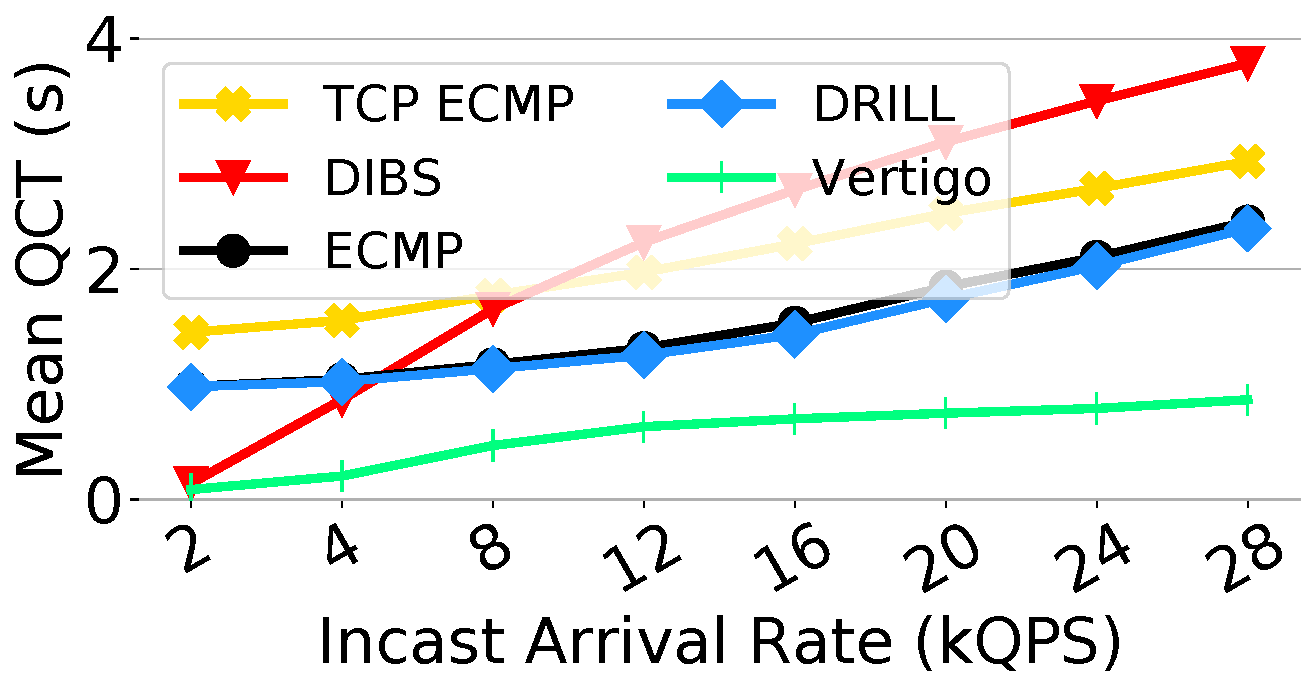
\includegraphics[width=0.98\linewidth]{figs/burst80.pdf}
% 		\caption{80\% Overall Load}
% 		\label{fig:burstiness80}
% 	\end{subfigure}
% 	\caption{Tweaking the degree of burstiness by gradually increasing the Incast arrivals and affixing the overall offered load.}
% 	\label{fig:burstiness}
% \end{figure*}




We evaluate Vertigo using large-scale OMNET++ simulations \cite{omnet} and microbenchmarks on a physical testbed using our prototype host component implementation.\footnote{Vertigo artifacts for large-scale simulations, host implementation, and switch scheduler abstraction are publicly available at \url{https://github.com/hopnets/vertigo-artifacts}.} We briefly summarize our findings:
%\begin{compactitem}
\begin{compactitem}
    \item Our large-scale simulations demonstrate that, using the DCTCP congestion control under 85\% offered load, Vertigo reduces the average incast query completion times by 66\%, 65\%, and 77\% compared to ECMP, DRILL, and DIBS, respectively (\S\ref{sec:large}).
    \item We show that combining Vertigo with Swift's state-of-the-art congestion control can significantly reduce the packet loss under bursty traffic (85\% load) and achieve 32$\times$, and 10$\times$ improvement over Swift+DRILL in query completion times and flow completion times, respectively  (\S\ref{sec:large}).
    \item We analyze the impact of each individual component of Vertigo and show how the combination of selective deflection, SRPT forwarding, re-transmission boosting, and receiver-side ordering achieves strong burst-tolerance (\S\ref{sec:component}).
%\end{compactitem}
\end{compactitem}
% After reporting the experiment setup in \S\ref{sec:setup}, we present the results for large-scale incast scenarios in \S\ref{sec:large}, showing that Vertigo outperforms widely deployed  alternatives in different offered loads, different degrees of burstiness, and different incast configurations. Next, we dive into Vertigo's design, evaluating each individual component in \S\ref{sec:component}. Our results indicate that each component plays a key role in achieving superior performance under incast traffic. Finally, we report the parameter sensitivity analysis in \S\ref{sec:parameter} and testbed experiments in \S\ref{sec:testbed}.

\begin{table}[t]
\centering
\small{

\begin{tabular}{l||l|l|l}
Setting                 & Min & Max  & Default \\ \hline \hline
Background Load \% \cite{hpcc, dibs, timely}     & 15  & 95   & \textbf{50}      \\
Incast QPS \cite{dibs}             & 2000  & 28000 & \textbf{4000}     \\
Incast Scale \cite{dibs, tlt}           & 50  & 450  & \textbf{100}      \\
Incast flow size (kB) \cite{dibs}  & 1   & 180  & \textbf{40}      \\
% MAX TTL  \cite{dibs}               & 10  & 250  & \textbf{250}      \\
Reordering timeout ($\mu s$) & 120 & 1080 & \textbf{360}  
\end{tabular}
% \vspace{-0.2cm}
\caption{\small{Parameter ranges used in Vertigo evaluation.}}
\label{tab:param}
\vspace{-0.6cm}
}
\end{table}

\subsection{Simulation Setup}
\label{sec:setup}
\textbf{Network Topologies.} We perform our simulations on a two-tiered leaf-spine topology consisting of 4 core switches, 8 aggregate switches, and 320 servers. The switch links have 40 Gbps bandwidth and the servers are connected to ToRs using 10 Gbps links. Each switch port has 300 kB buffer capacity \cite{dibs, ecnmultiqueue}. We also validate our findings against an equivalent fat-tree \cite{fattree} network ($k=8$) with 128 servers and 80 switches.
% \Erfan{We perform our simulations on (1) a two-tiered leaf-spine topology consisting of 4 core switches, 8 aggregate switches, and 320 servers. The switch links have 40Gbps bandwidth and the servers are connected to ToRs using 10Gbps links, (2) an equivalent fat-tree \cite{fattree} network ($k=8$) with 128 servers and 10Gbps links in the entire network.
% Each switch port has 300KB buffer capacity \cite{dibs, ecnmultiqueue}.}

\textbf{Workloads.} For the background load, we run widely deployed, public datacenter traffic traces, \ie Facebook's cache follower, Facebook's data mining, and Google's web search, for interarrival times and flow size distributions \cite{social, dctcp}. We scale the flow interarrival times to vary the load. For generating microbursts, we implement an incast application in which some randomly selected clients periodically send queries to a set of servers, also selected at random, that all reply to the queries simultaneously. To vary the level of traffic burstiness, we change three parameters: (a) the incast \emph{scale}, \ie the number of servers that each client sends a query to, (b) the number of incast queries per second (QPS), \ie the rate at which the destinations initiate incast queries and (c) the individual incast flow size. We set the simulation time limit of the experiments to 5 seconds.
% \Erfan{ and only report the results for systems that complete at least 50\% of the flows.}
% \fixme{\textbf{[COVERED]} add simulation time here.}

\textbf{Alternative approaches.} We compare Vertigo against in-network solutions like ECMP, the default load-balancing scheme widely used in datacenters, DRILL \cite{drill}, a micro load-balancer with per-packet load distribution decisions, and DIBS \cite{dibs}, a random packet deflection technique. For transport and congestion control, we combine the above alternatives with TCP Reno \cite{newreno}, DCTCP \cite{dctcp}, and Swift \cite{swift}. We also evaluate Vertigo's performance with alternative packet marking and scheduling disciplines. 
%We present the results in the following sections.

\textbf{Parameter settings.} Table \ref{tab:param} lists the parameters for large-scale simulations. Unless explicitly stated otherwise, we use the default values for all experiments, run DCTCP with the marking threshold of 65 as our default transport protocol, set Vertigo's deflection and load-balancing factors (power of n) to 2, TCP's initial window to 10 packets, and TCP's initial RTO to 1s and minRTO to 10\emph{ms} to closely follow the parameter settings reported in \cite{dctcp, dibs}. Lastly, we configure Swift according to the guidelines provided in \cite{swift}. All other parameters are default INET settings \cite{inet}. 

\subsection{Large-scale Event-driven Simulations}
\label{sec:large}
We evaluate Vertigo under various incast and non-incast traffic settings by comparing it to widely deployed and the state-of-the-art techniques. We collect and report the response times, flow completion times (FCT), query completion times (QCT), application goodput, and some lower-level metrics like packet drops, reordering, and RTTs.
% and \sepehr{length of the paths packets traverse.}
%path-stretch.
% We find that Vertigo can successfully overcome the challenges faced by random packet deflection and substantially increase the tolerance of datacenter networks against micro-scale congestion. 



\begin{figure*}[th!]
	\centering
	\begin{subfigure}[t]{.32\linewidth}
	\centering
	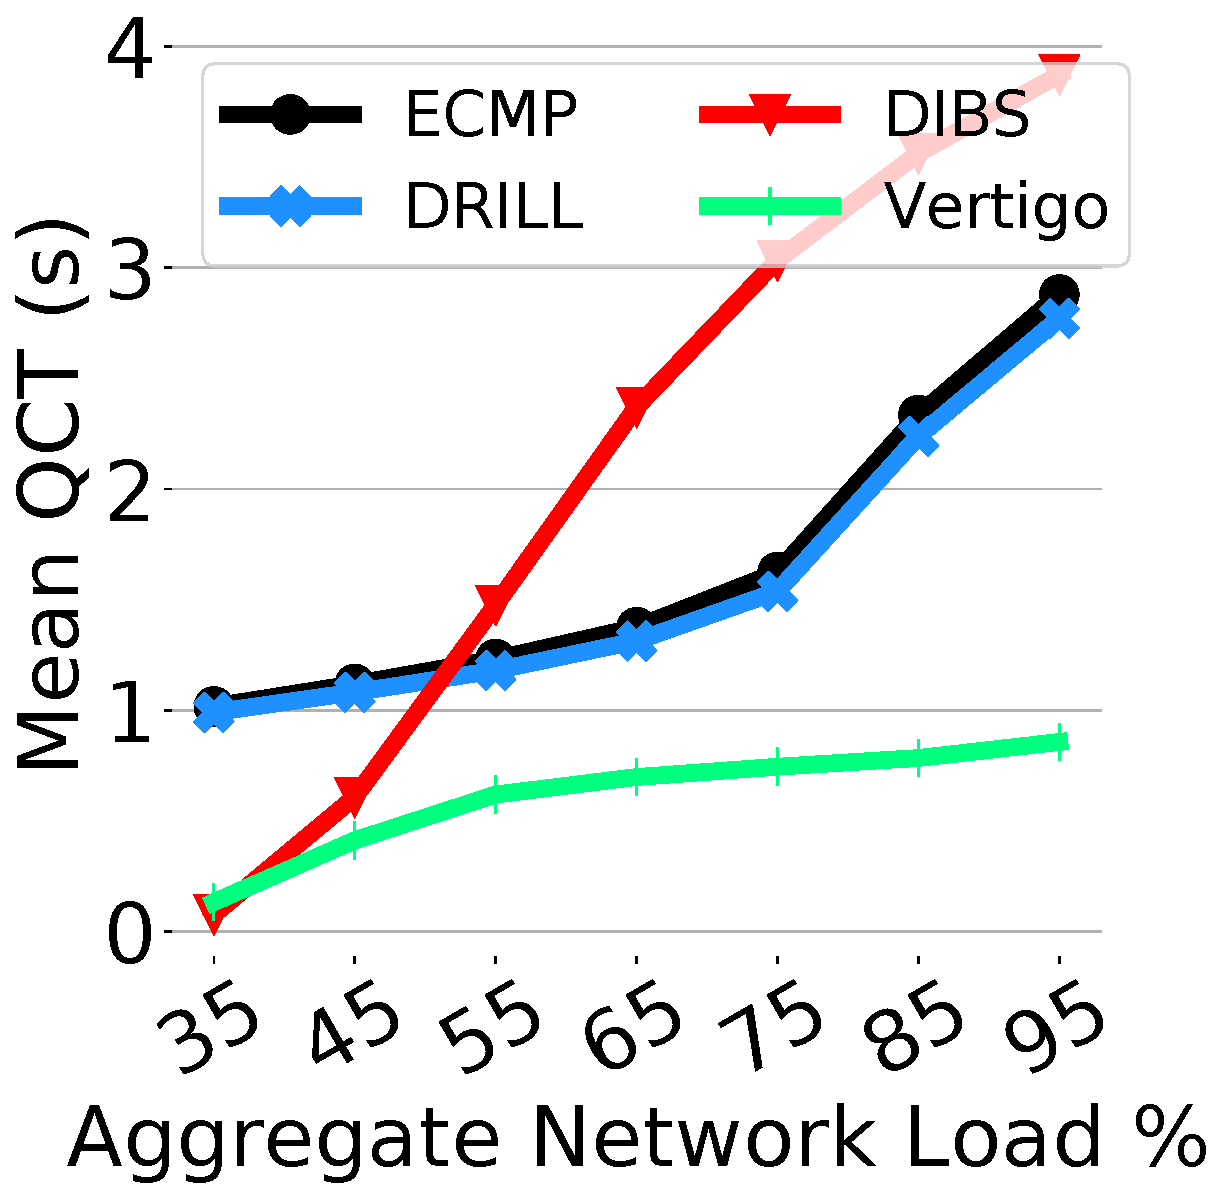
\includegraphics[width=0.85\linewidth, height=2.4cm]{figs/qps25.pdf}
	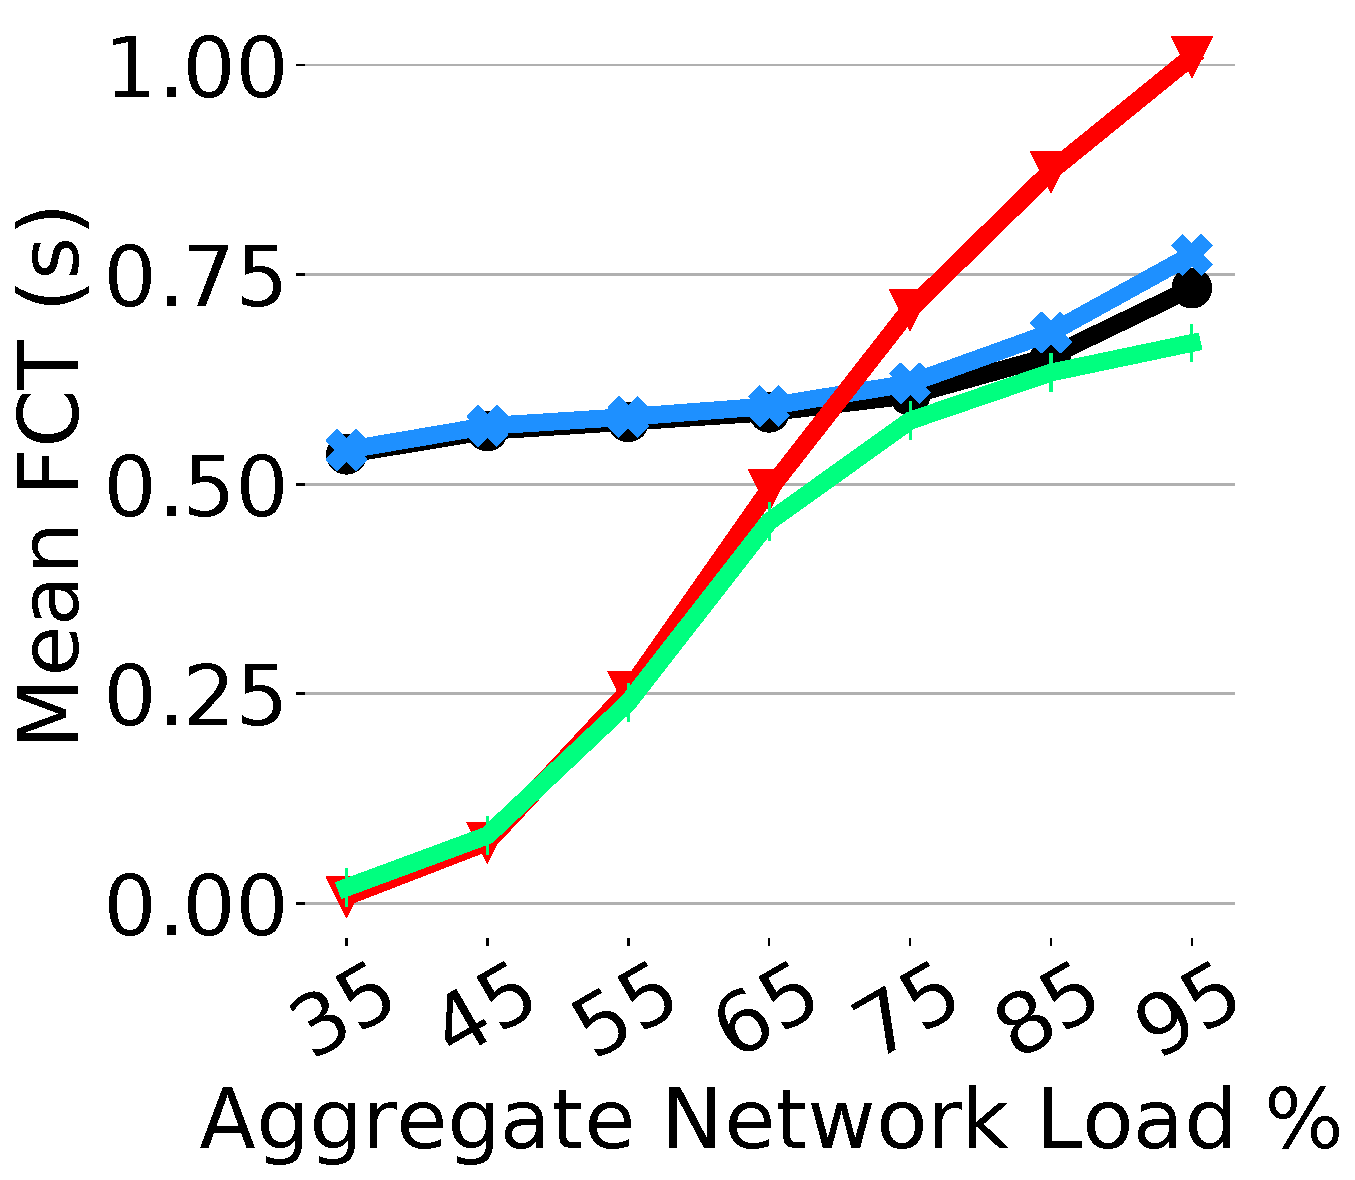
\includegraphics[width=0.85\linewidth]{figs/qps25fct.pdf}
	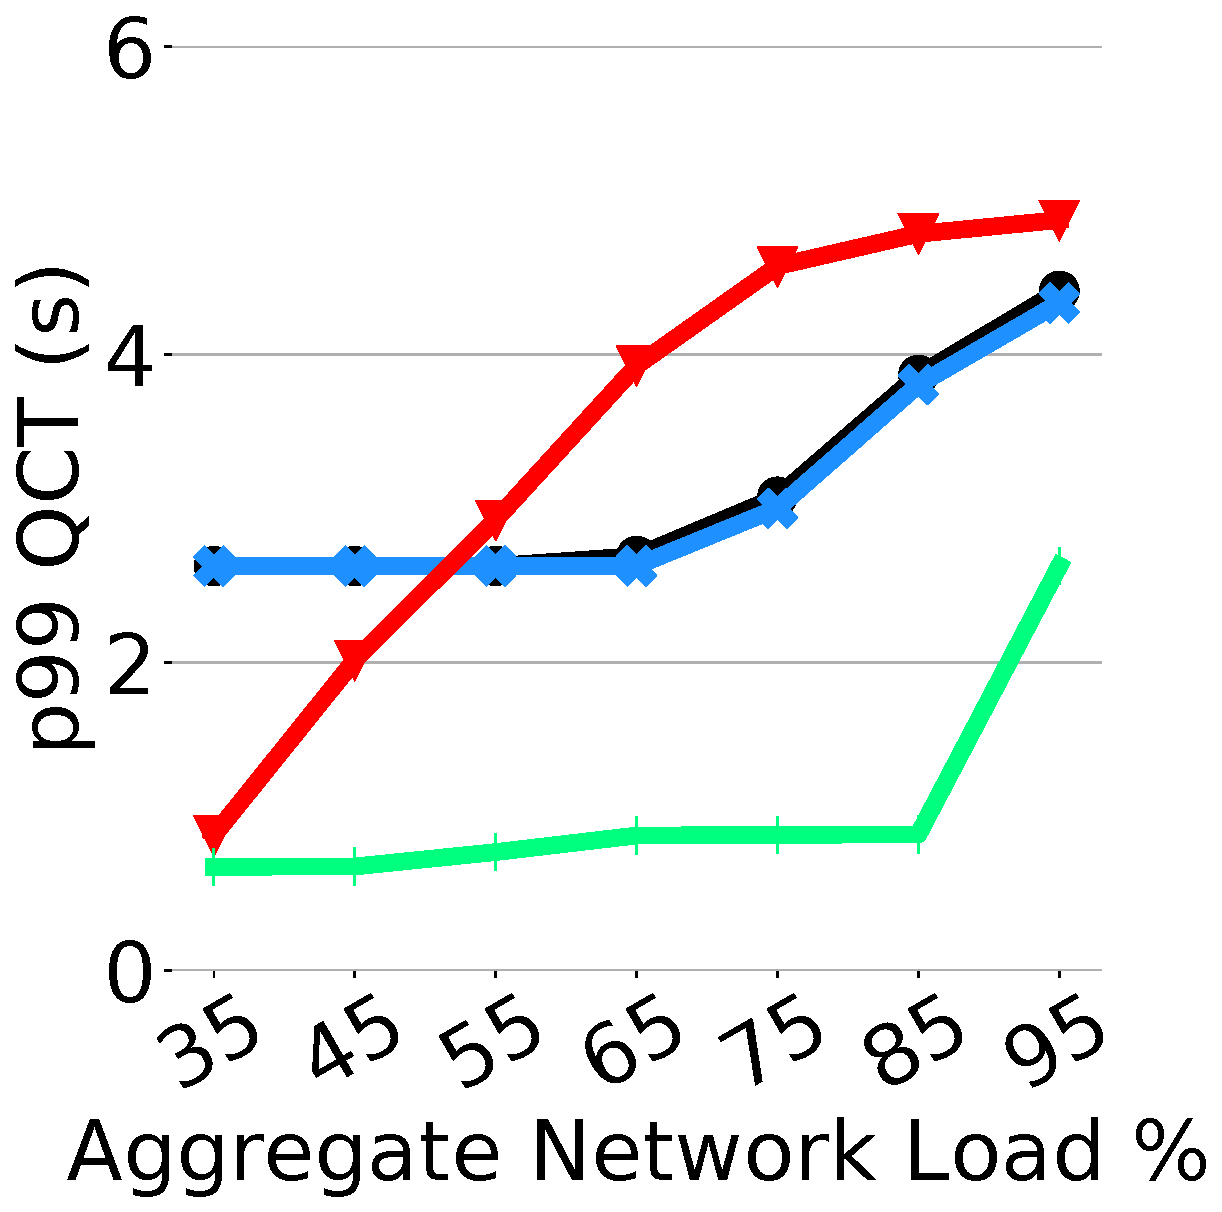
\includegraphics[width=0.85\linewidth]{figs/qps25p99qct.pdf}
	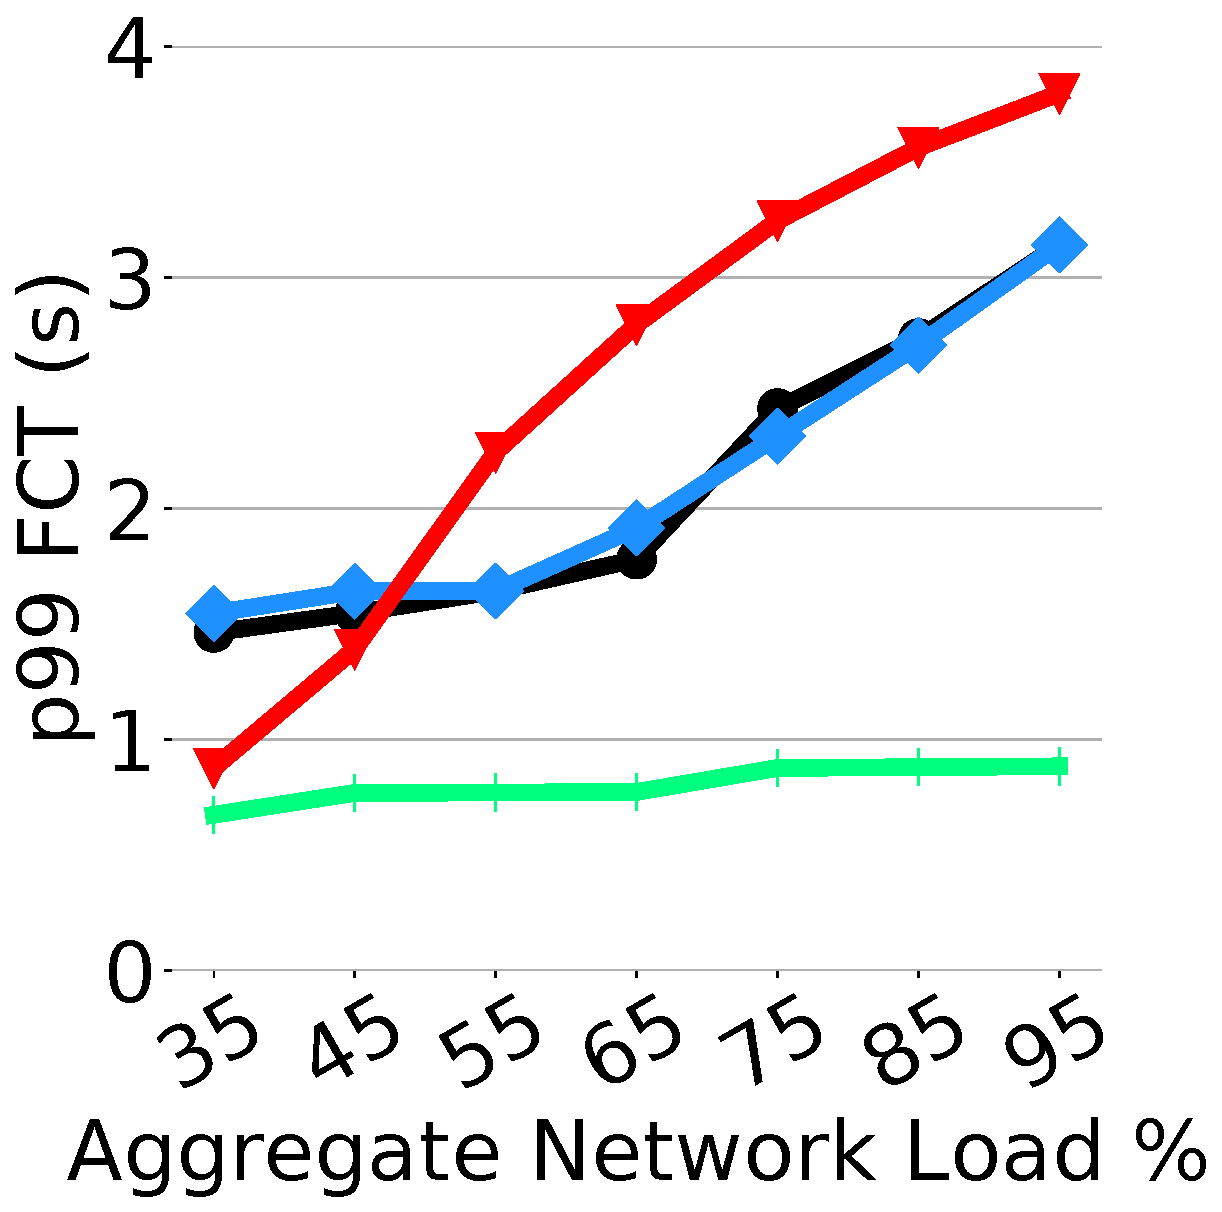
\includegraphics[width=0.85\linewidth]{figs/qps25tcpp99fct.pdf}
		\caption{\small{25\% BG Load}}
		\label{fig:qps25}
	\end{subfigure}
	\rulesep
	\begin{subfigure}[t]{.32\linewidth}
	\centering
	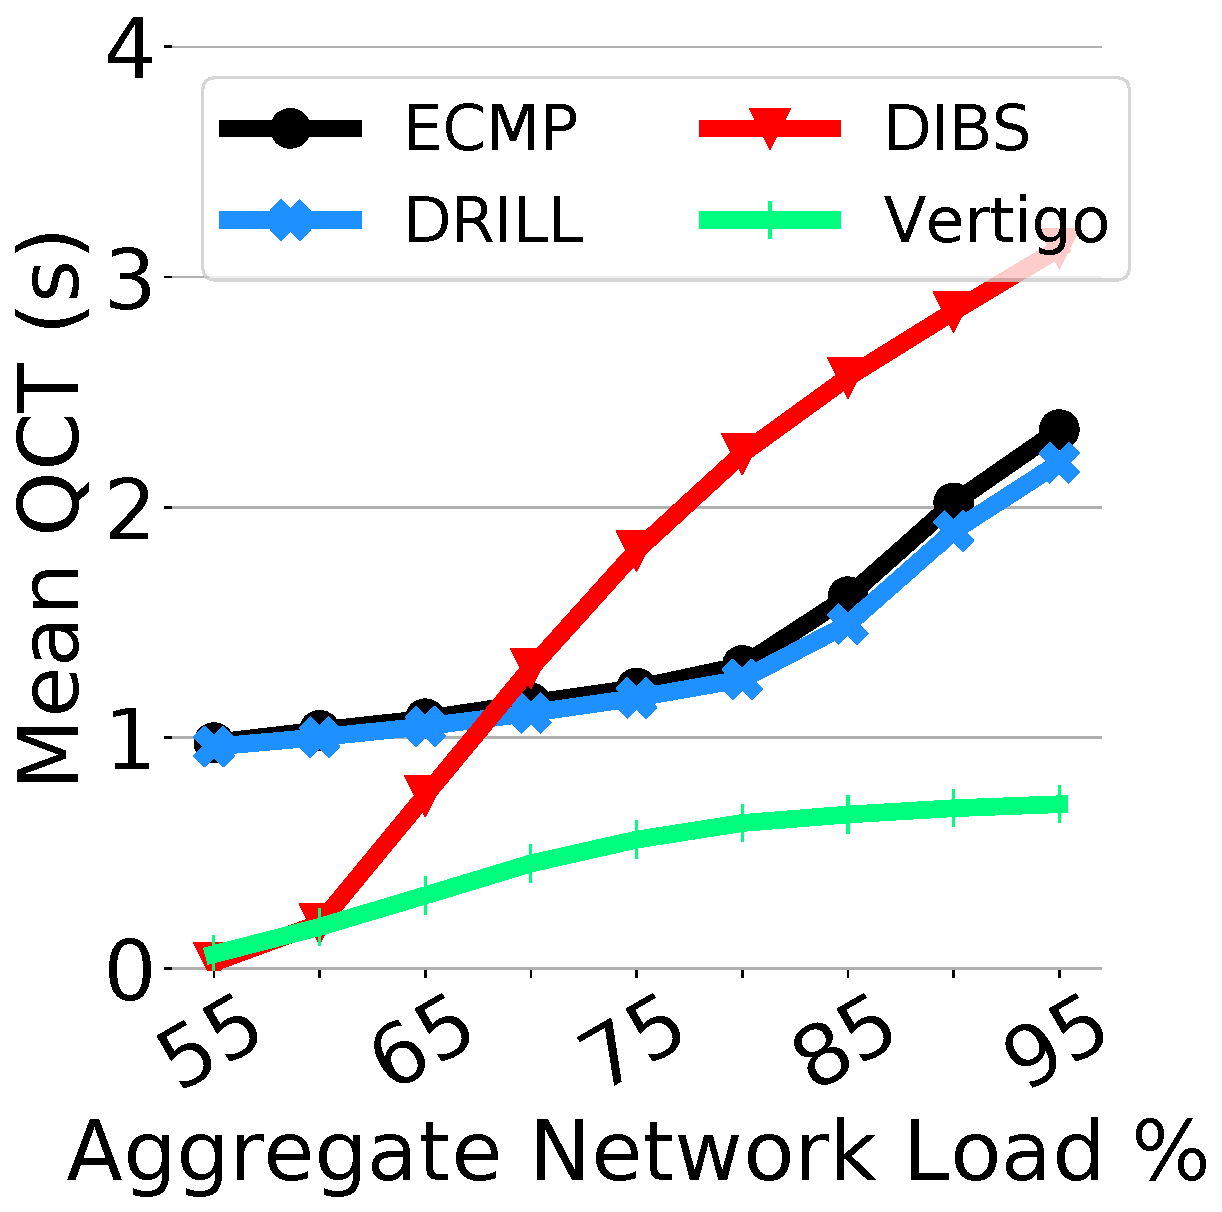
\includegraphics[width=0.85\linewidth, height=2.4cm]{figs/qps50.pdf}
	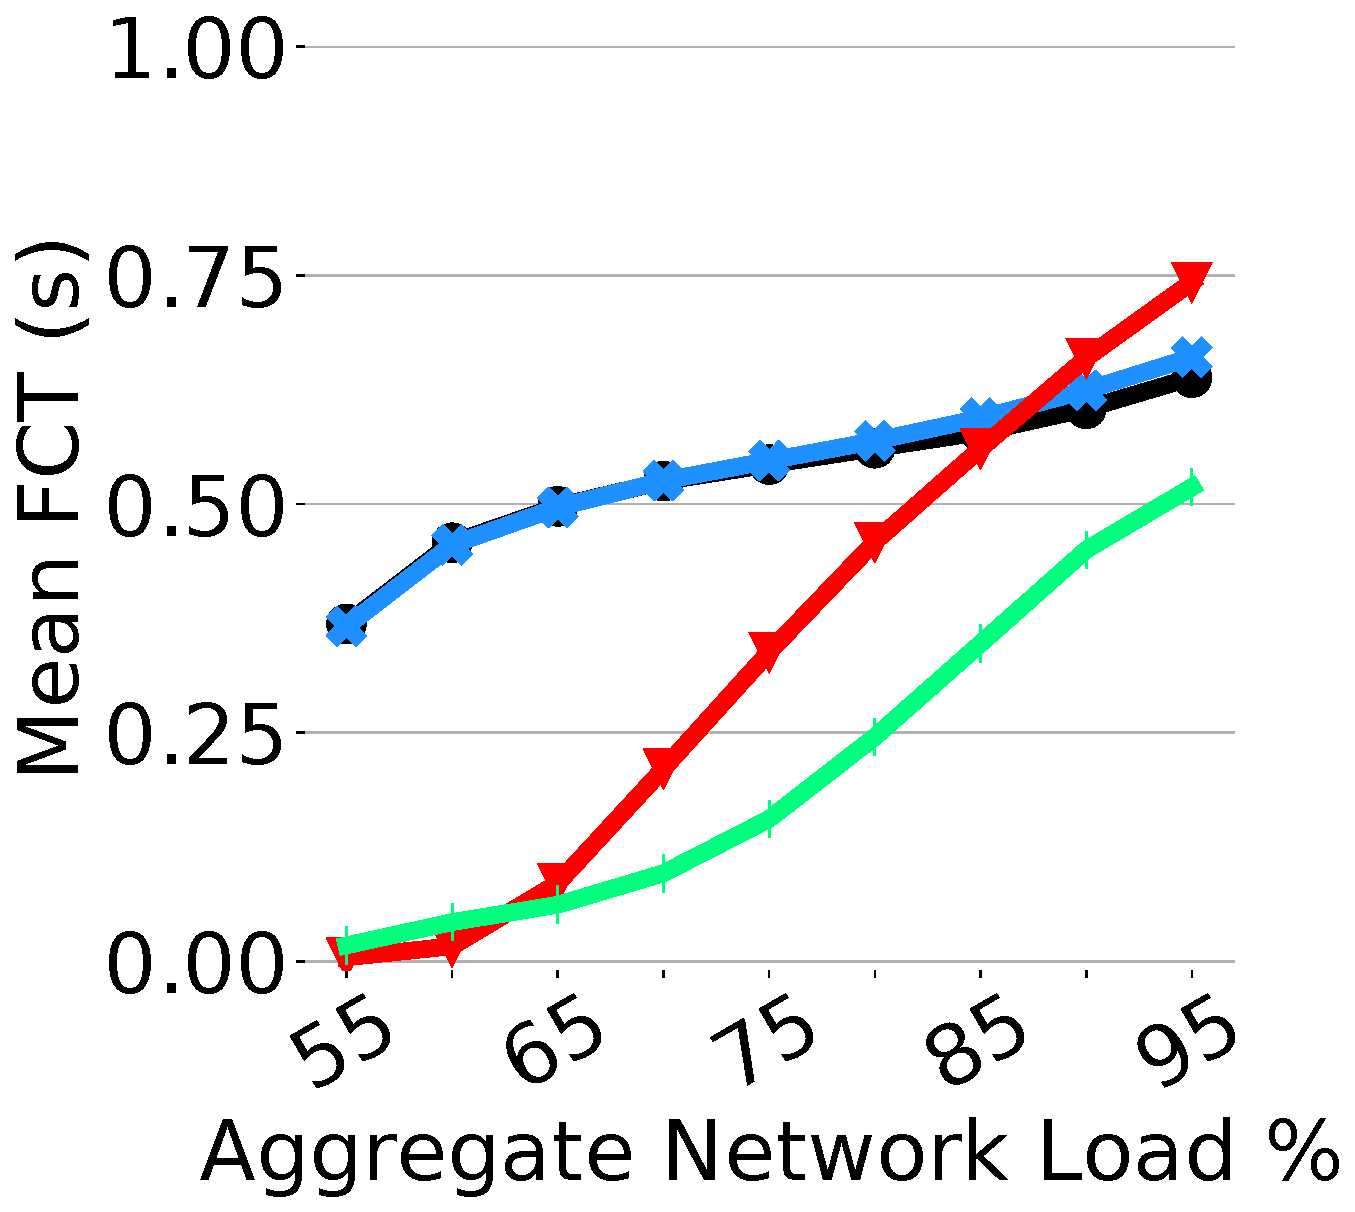
\includegraphics[width=0.85\linewidth]{figs/qps50fct.pdf}
	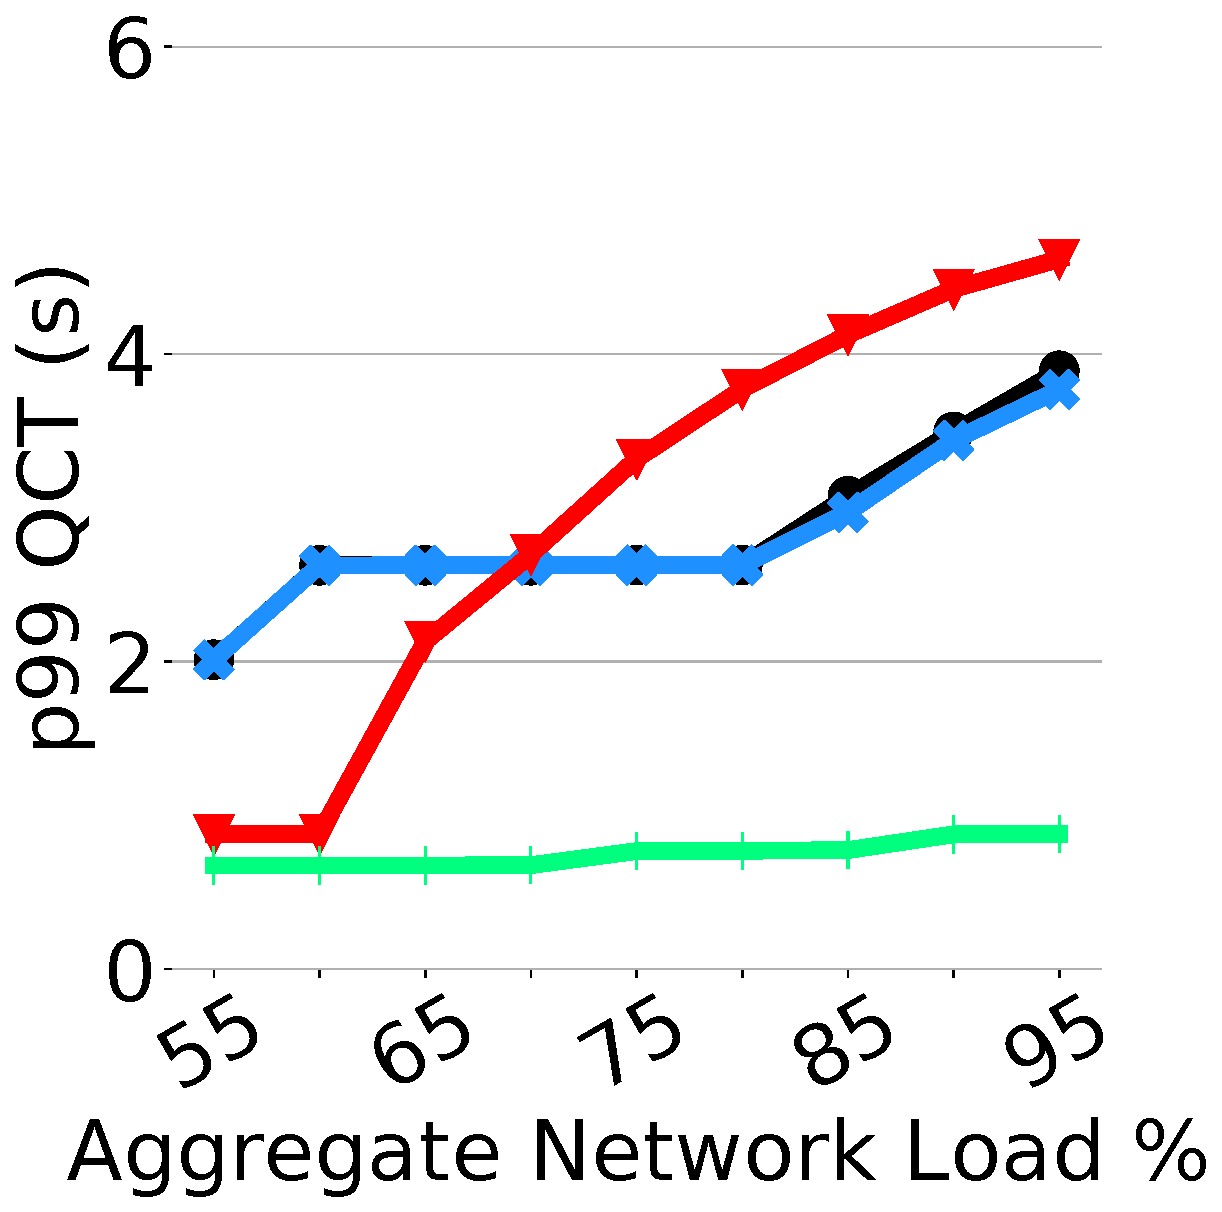
\includegraphics[width=0.85\linewidth]{figs/qps50_p99qct.pdf}
	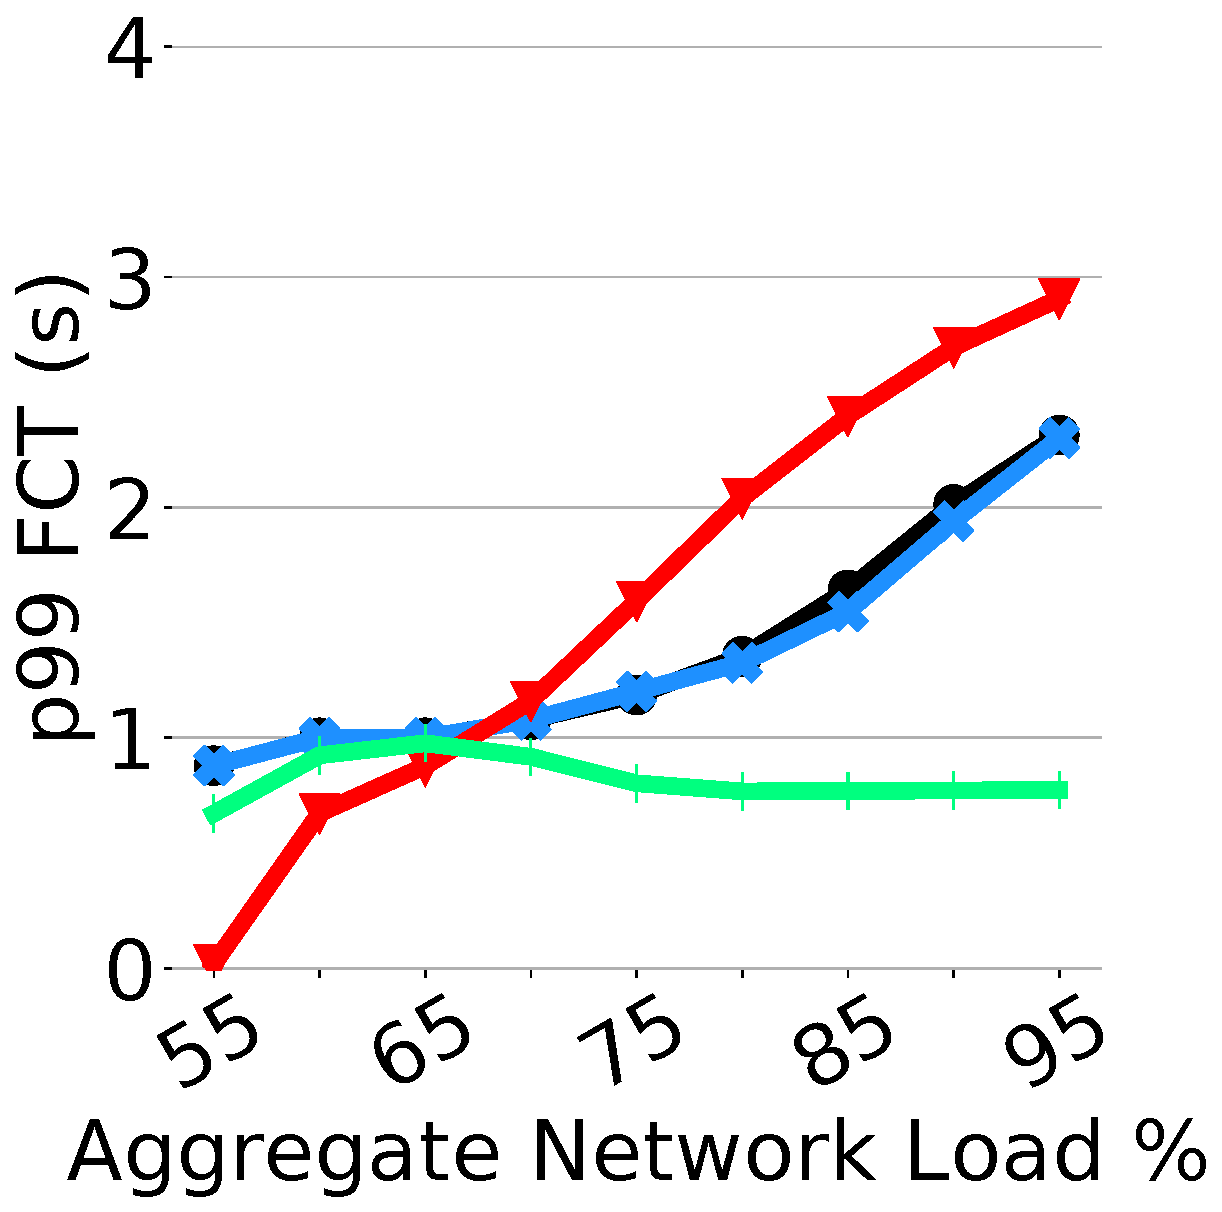
\includegraphics[width=0.85\linewidth]{figs/qps50p99fct.pdf}
		\caption{\small{50\% BG Load}}
		\label{fig:qps50}
	\end{subfigure}
	\rulesep
	\begin{subfigure}[t]{.32\linewidth}
	\centering
	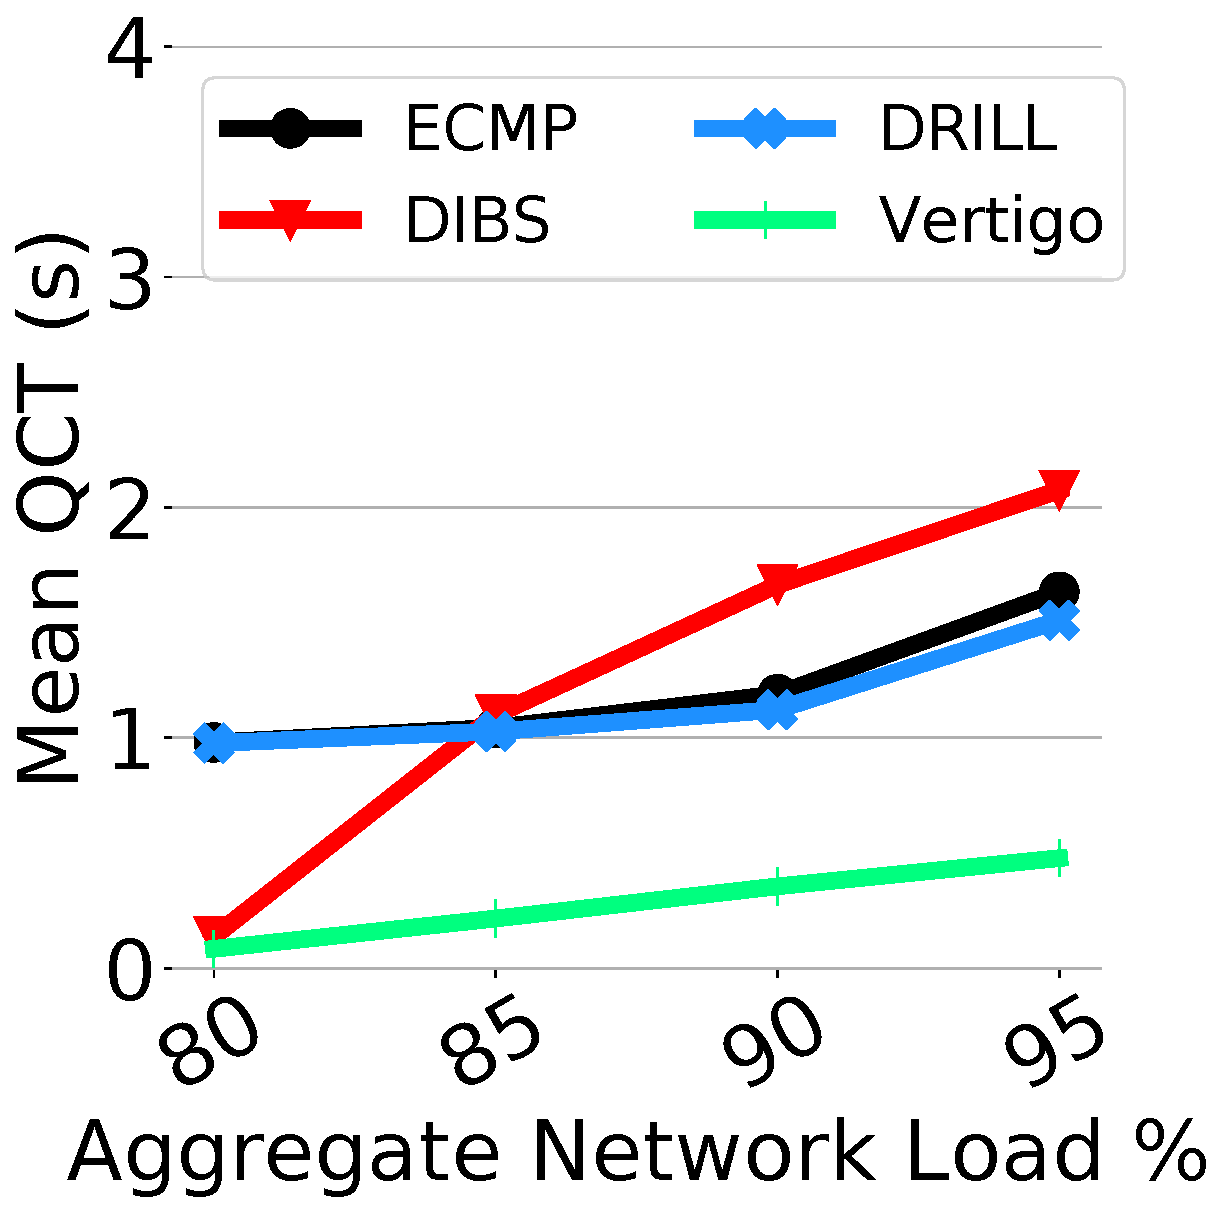
\includegraphics[width=0.85\linewidth, height=2.4cm]{figs/qps75.pdf}
	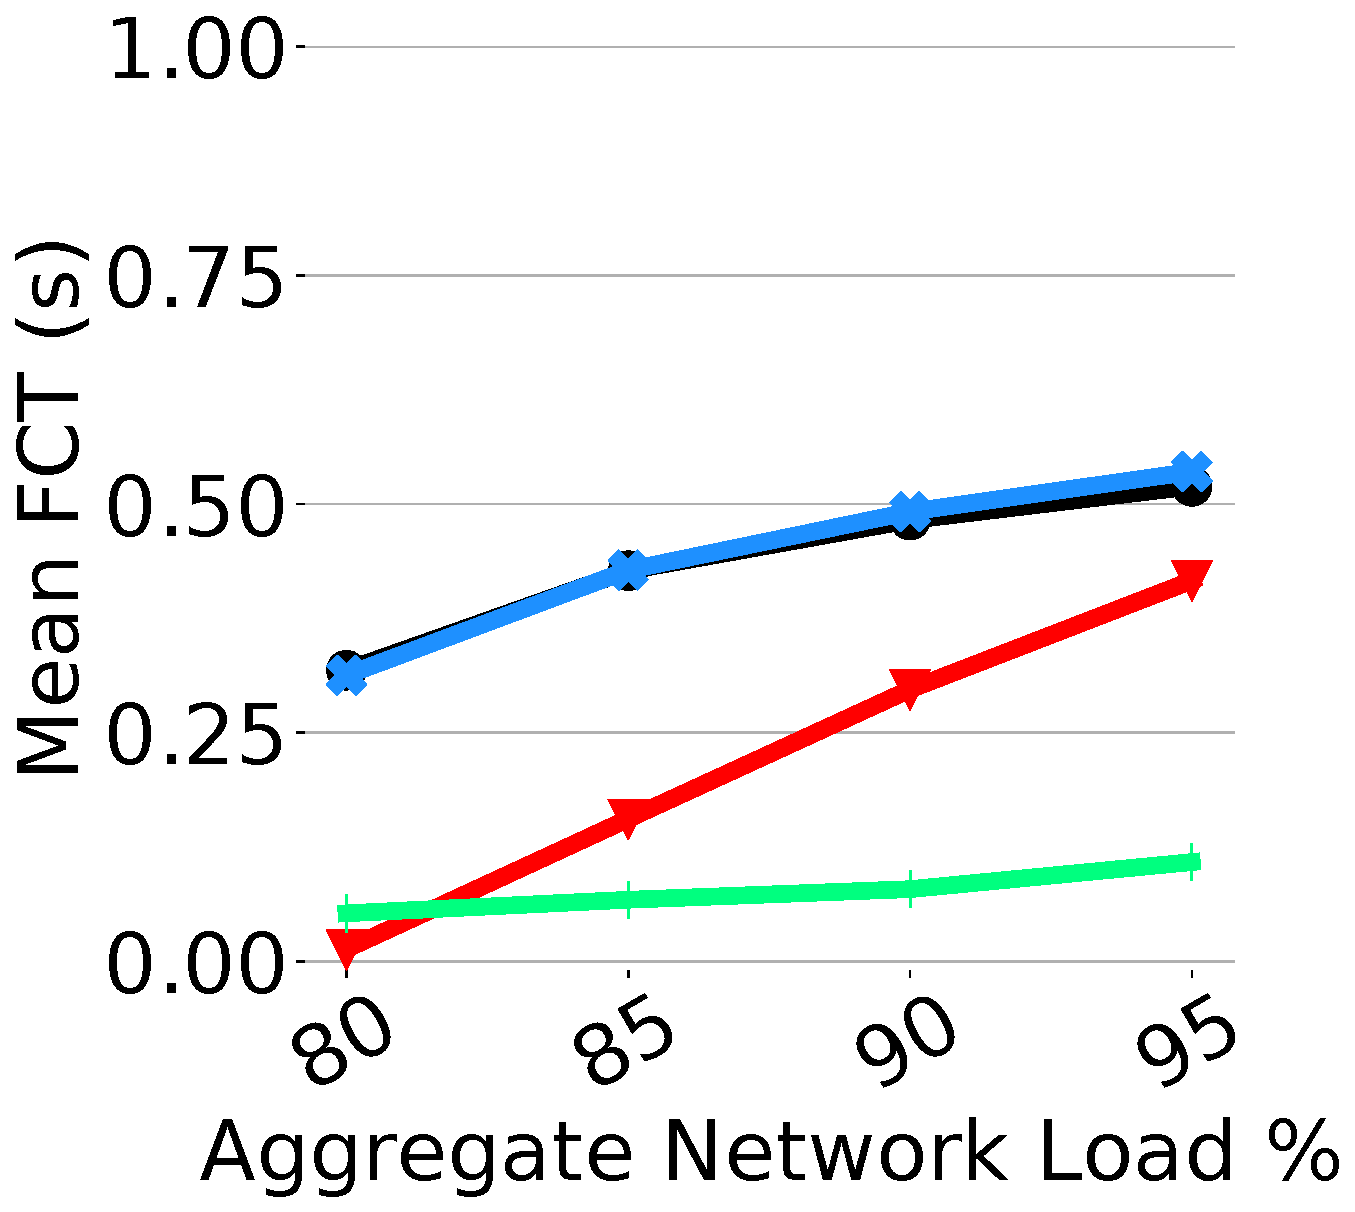
\includegraphics[width=0.85\linewidth]{figs/qps75fct.pdf}
	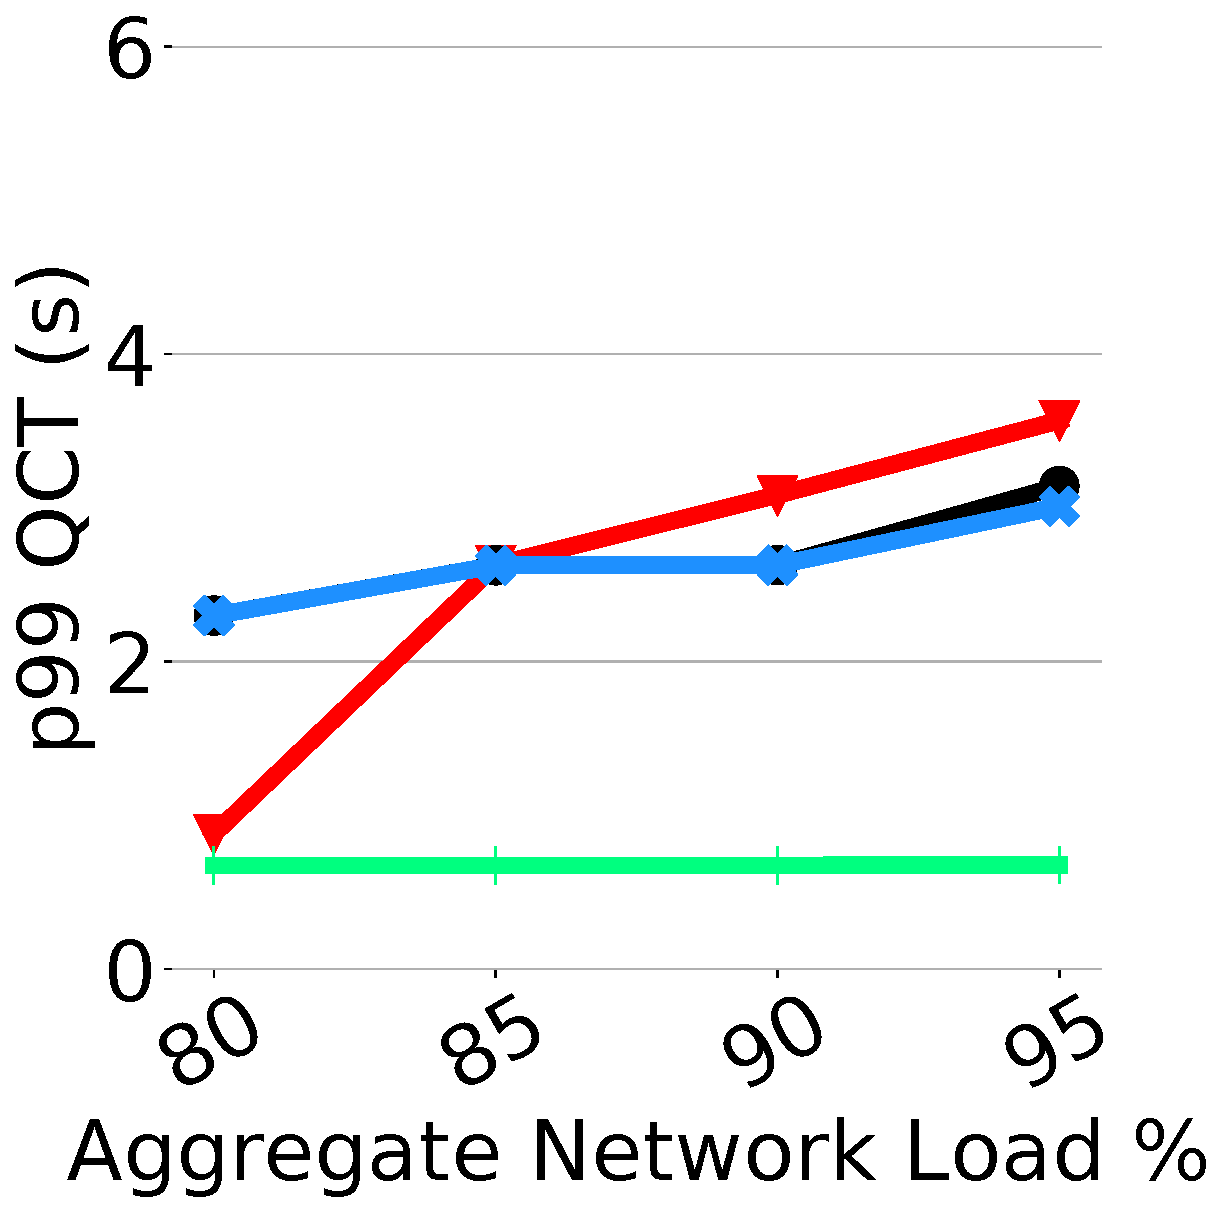
\includegraphics[width=0.85\linewidth]{figs/qps75_p99qct.pdf}
	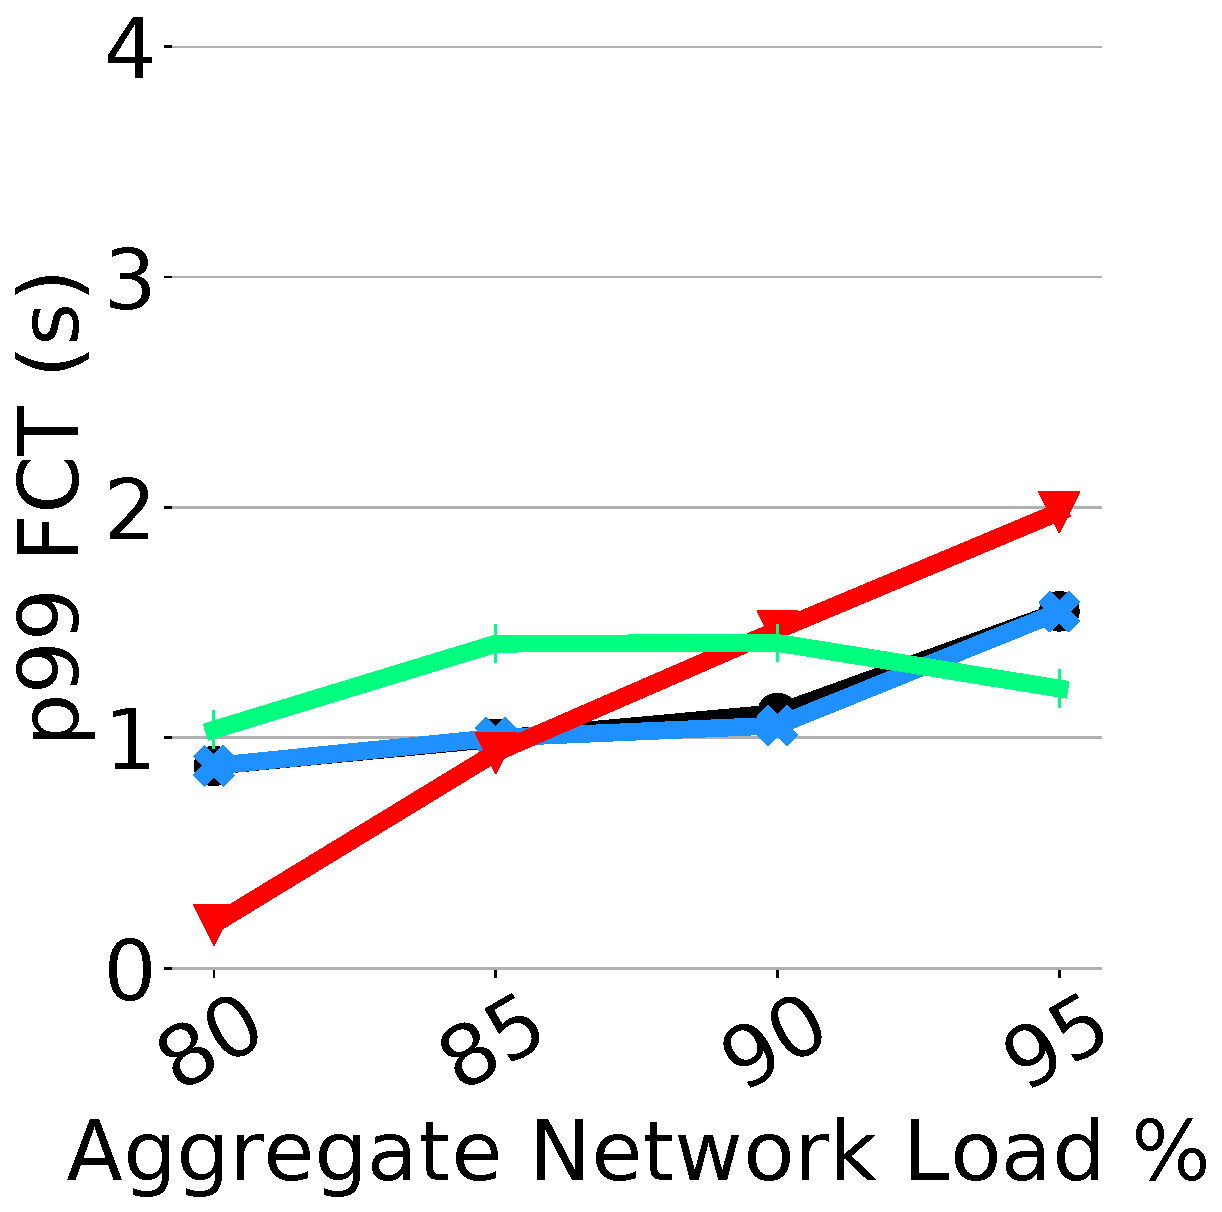
\includegraphics[width=0.85\linewidth]{figs/qps75p99fct.pdf}
		\caption{\small{75\% BG Load}}
		\label{fig:qps75}
	\end{subfigure}
% 	\begin{subfigure}[t]{.32\linewidth}
% 	\centering
% 	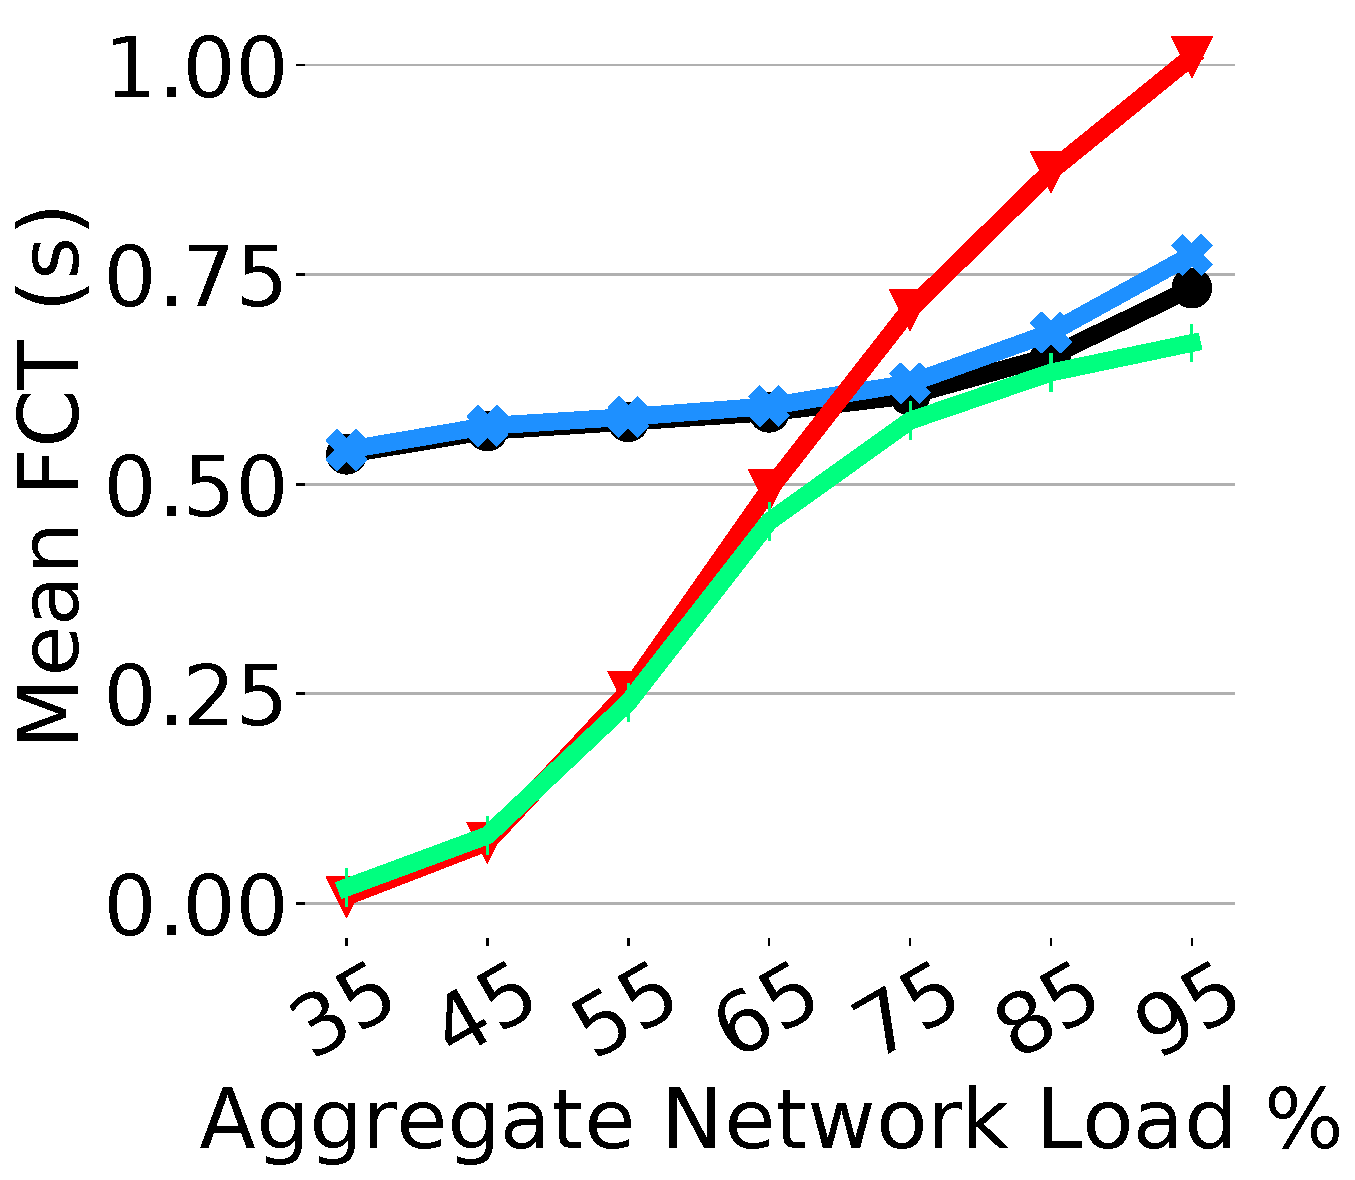
\includegraphics[width=0.98\linewidth]{figs/qps25fct.pdf}
% 		\caption{\small{25\% BG Load - FCT}}
% 		\label{fig:qps25fct}
% 	\end{subfigure}
% 	\begin{subfigure}[t]{.32\linewidth}
% 	\centering
% 	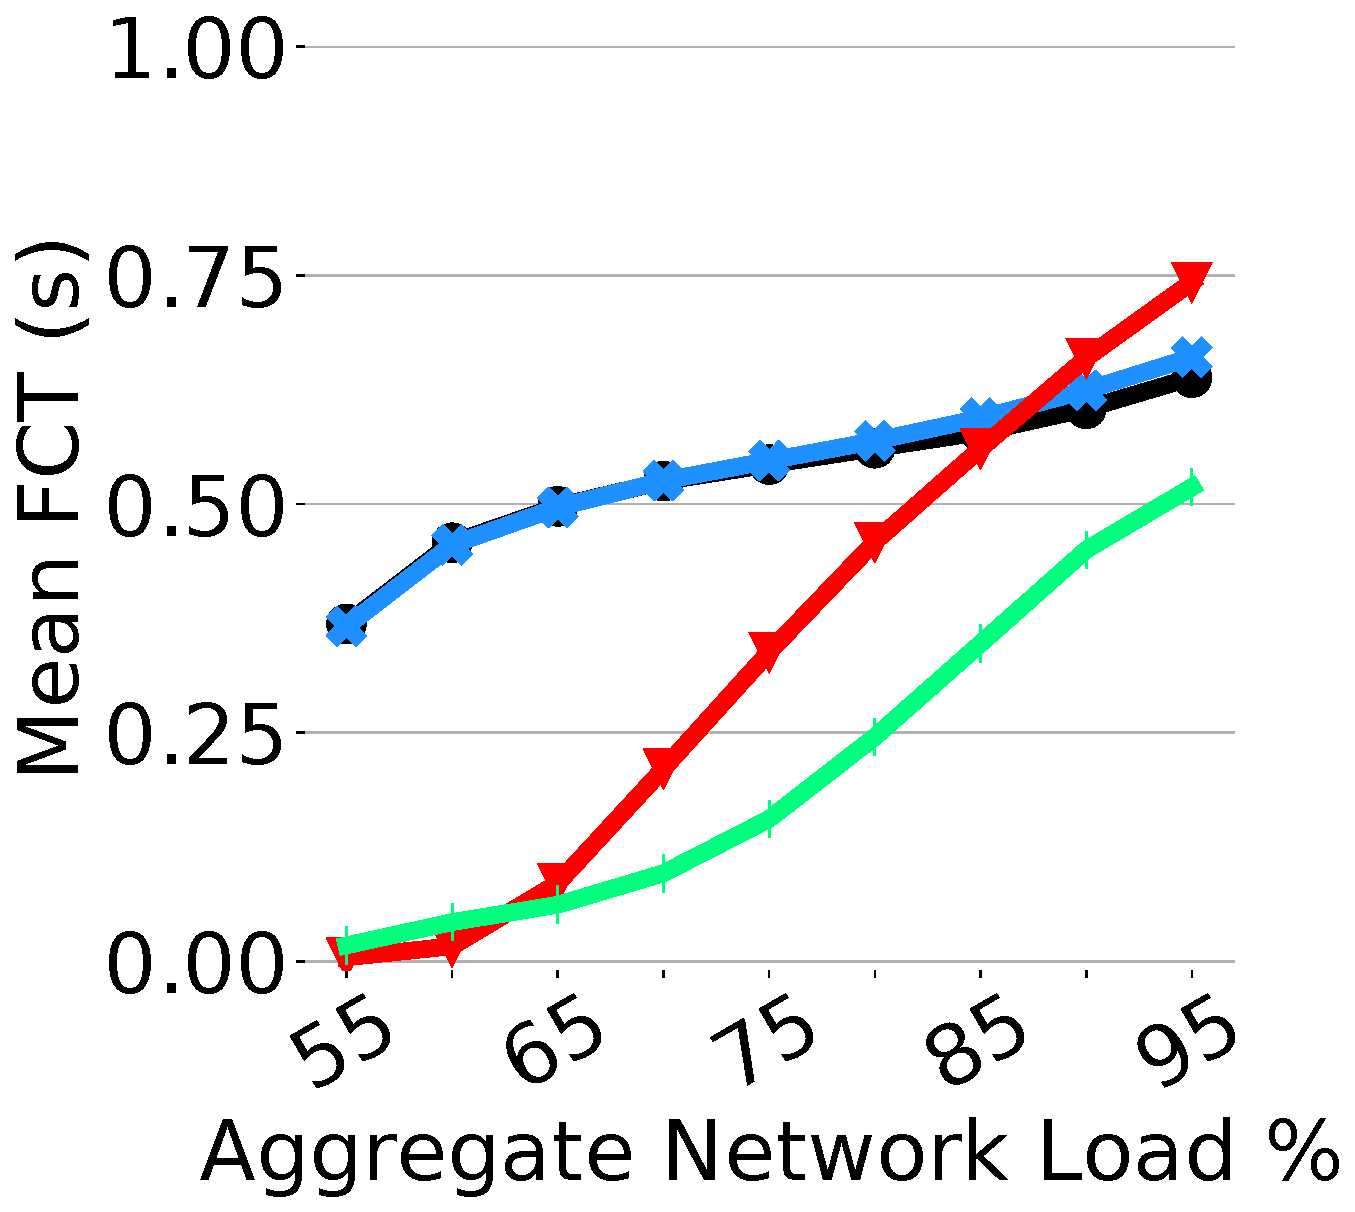
\includegraphics[width=0.98\linewidth]{figs/qps50fct.pdf}
% 		\caption{\small{50\% BG Load - FCT}}
% 		\label{fig:qps50fct}
% 	\end{subfigure}
% 	\begin{subfigure}[t]{.32\linewidth}
% 	\centering
% 	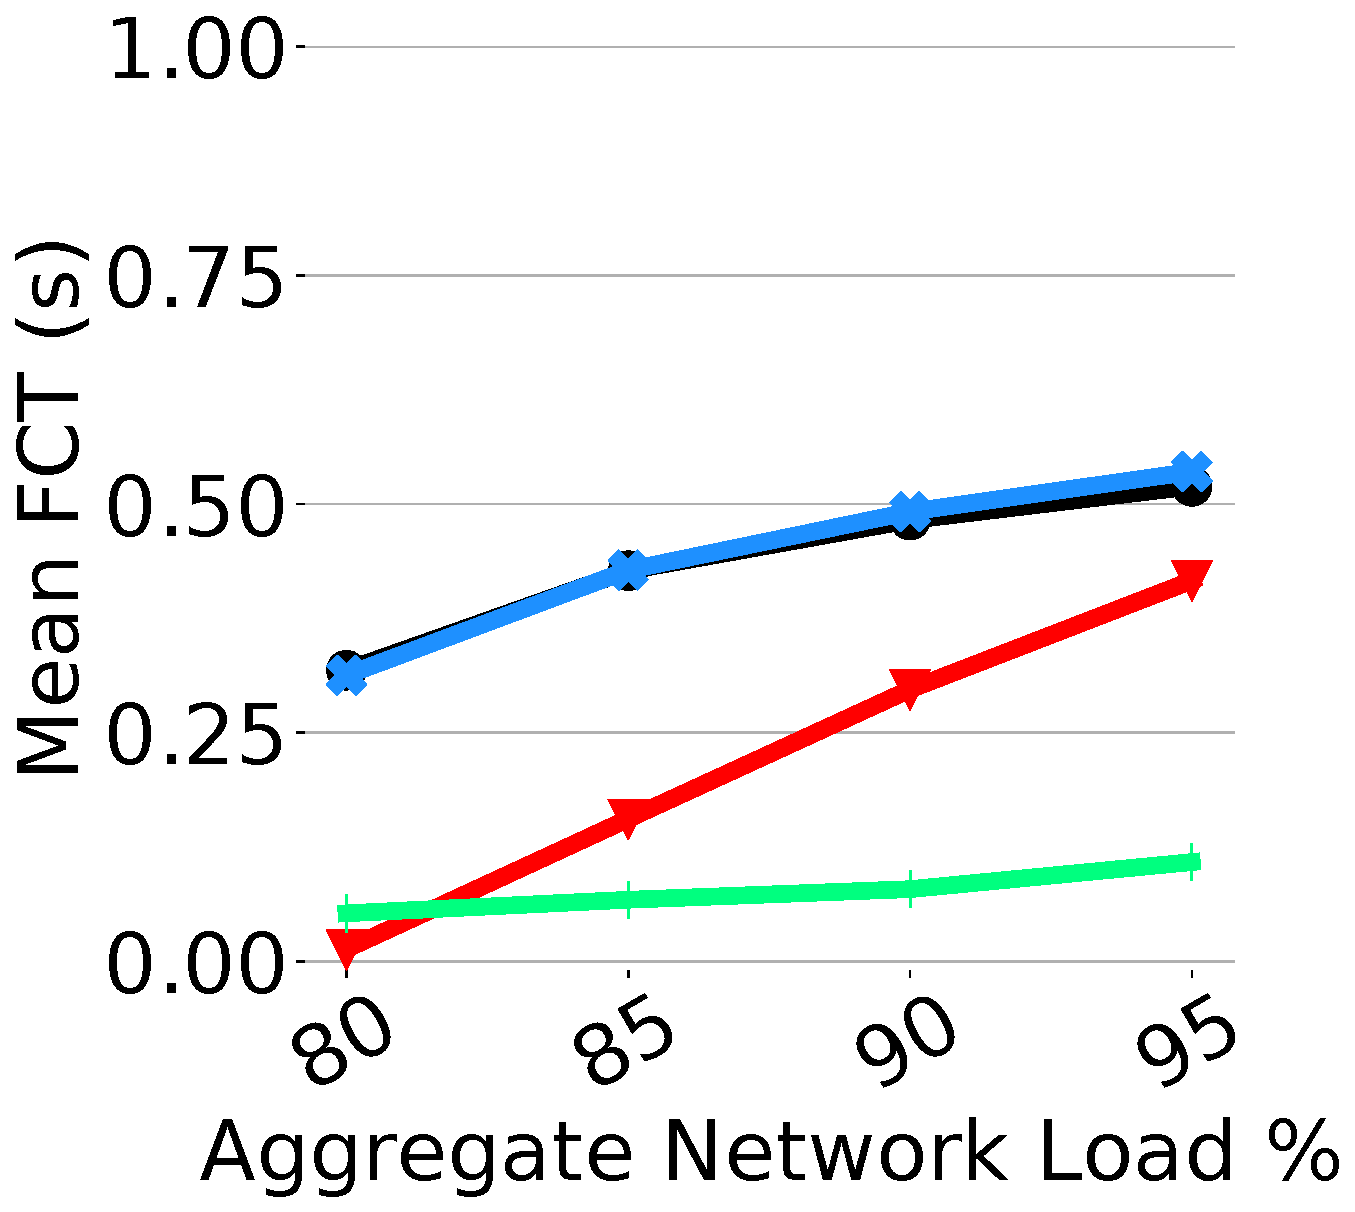
\includegraphics[width=0.98\linewidth]{figs/qps75fct.pdf}
% 		\caption{\small{75\% BG Load - FCT}}
% 		\label{fig:qps75fct}
% 	\end{subfigure}
	\caption{\small{Vertigo achieves a steady QCT performance under various load distributions when all systems use DCTCP as their transport. As the background load dominates the network, fewer packet drops lead to shorter query completion times.}}
	\label{fig:qps}
    % \vspace{-0.3cm}
\end{figure*}

\textbf{Vertigo offers superior performance under various degrees of load.}
In the first experiment, we gradually increase the incast event rate under three different degrees of background load, 25\%, 50\%, and 75\%.
The results, presented in Figure \ref{fig:qps}, clearly show the limitations of micro load balancing and random deflection. DRILL (a micro load balancer) cannot prevent last-hop bursts that are induced by incast. In practice, the majority of drops occur at the last hops \cite{jupiter, hpcc}. The performance of DIBS 
% (a random deflection technique) 
rapidly degrades under load, \eg with a 10\% increase in the overall load from 60\% (50\% background+10\% bursty workload) to 70\% (50\% background+20\% bursty workload), the mean QCT and FCT of DIBS increase 6-fold and 21-fold, respectively.
%  
In comparison, the performance of other techniques degrades much more gracefully under load, \eg the QCT and FCT of DRILL increase by 10\% and 16\%, respectively. Overall, neither micro load balancing nor deflection alone is effective under both low and high loads. Vertigo, in contrast, consistently delivers low FCT and QCT under all degrees of load including extreme loads, \eg under 90\% load (75\% background + 15\% incast load), Vertigo reduces the mean FCT of DRILL and DIBS by 5.1$\times$ and 2.7$\times$, respectively. The results also show that when the background load dominates the incast load, DIBS's 99$^{th}$ FCT percentile (p99) remains lower than other systems due to saving persistent background flows, however, this performance comes at the cost of higher incast query completion times compared to Vertigo.
%performance degradation under load is also more gradual than random deflection, \eg increasing the load from 60\% to 70\% increases Vertigo's mean FCT by 20\%.
% \sepehr{To quantify the path-stretch, we store the average number of hops packets traverse to reach their destination at end-hosts. Our results illustrate that, under 50\% offered load, applying random packet deflection increases the average number of hops traversed by 20\%.}
%
%Figure \ref{fig:qps} shows the results. As the overall load increases, systems that are vulnerable to packet loss experience prolonged query completion times. That is because these systems require many re-transmissions to complete a single query. In Vertigo, some packets get a second chance by being re-routed in the network. Even in the event of drops, the boosting mechanism employed in the marking component ensures that re-transmitted packets have a substantially increased chance of reaching their destination. The results demonstrate that packet re-transmission is reduced by up to 31\% when the boosting mechanism is enabled. The results also demonstrate that random deflection fails to keep up with the incast rate as DIBS's QCT performance starts to deteriorate when incast flows dominate the network. Finally, we observe that fine-grained load-balancing has but a negligible effect as its FCT performance barely exceeds 2\% of ECMP in all workloads. This indicates why even fine-grained load-balancing, per se, cannot help with incast traffic.

\begin{figure}
    	\begin{subfigure}[t]{.45\linewidth}
	\centering
	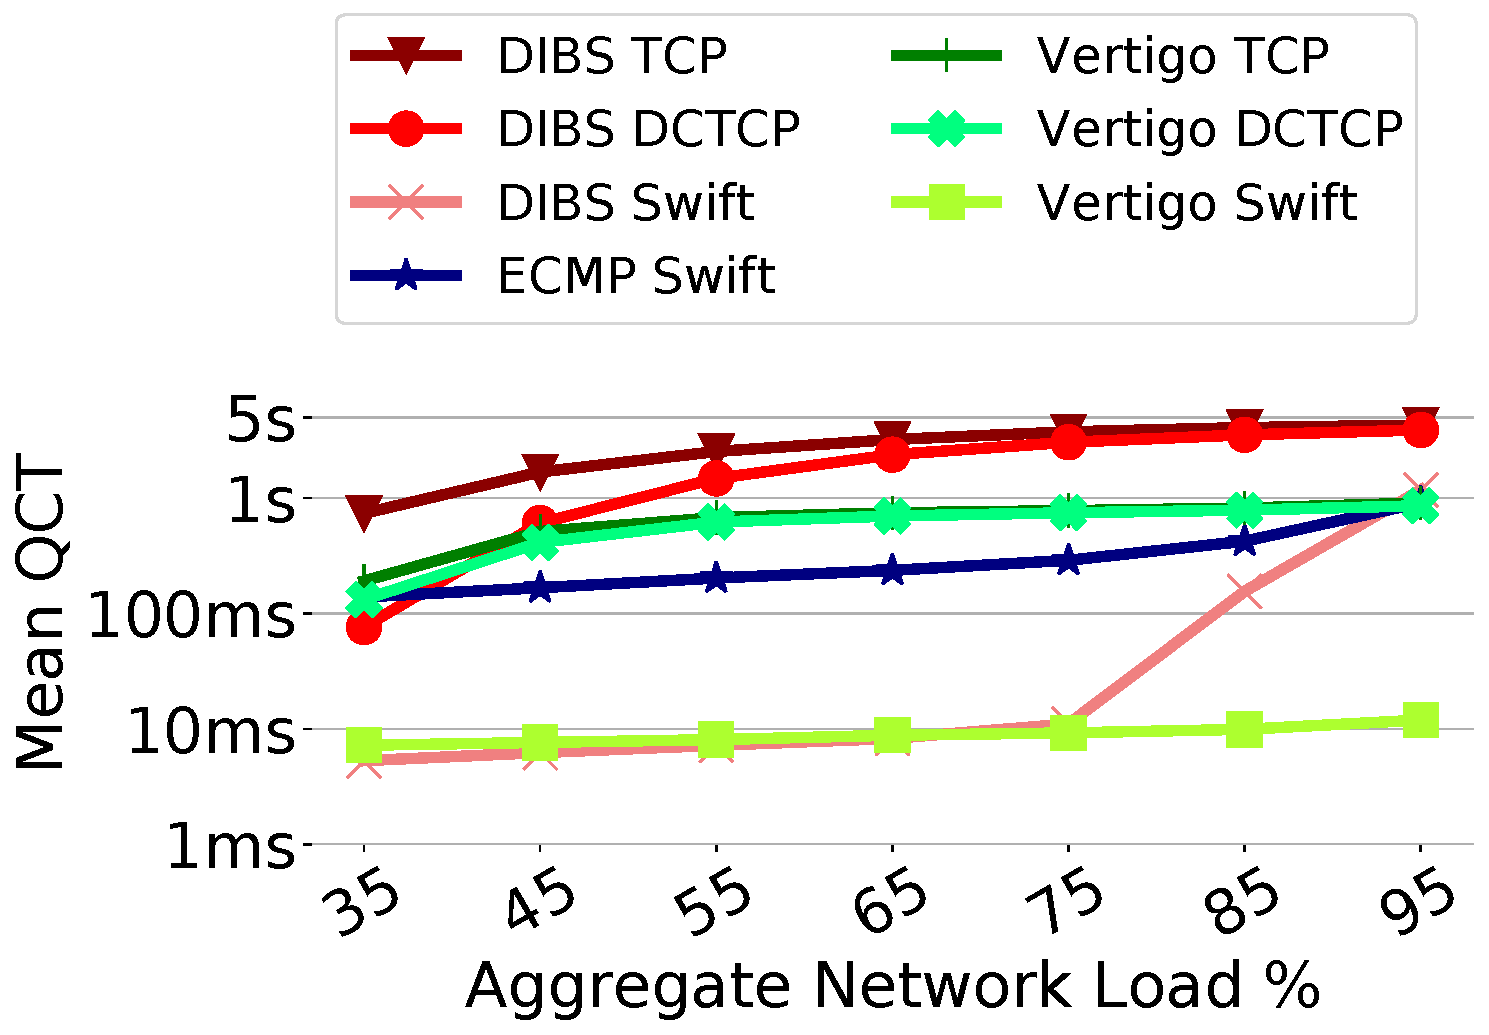
\includegraphics[width=0.98\linewidth]{figs/qps25tcpdctcpswift.pdf}
		\caption{\small{Mean QCT}}
		\label{fig:transport_qct}
	\end{subfigure}
	\begin{subfigure}[t]{.45\linewidth}
	\centering
	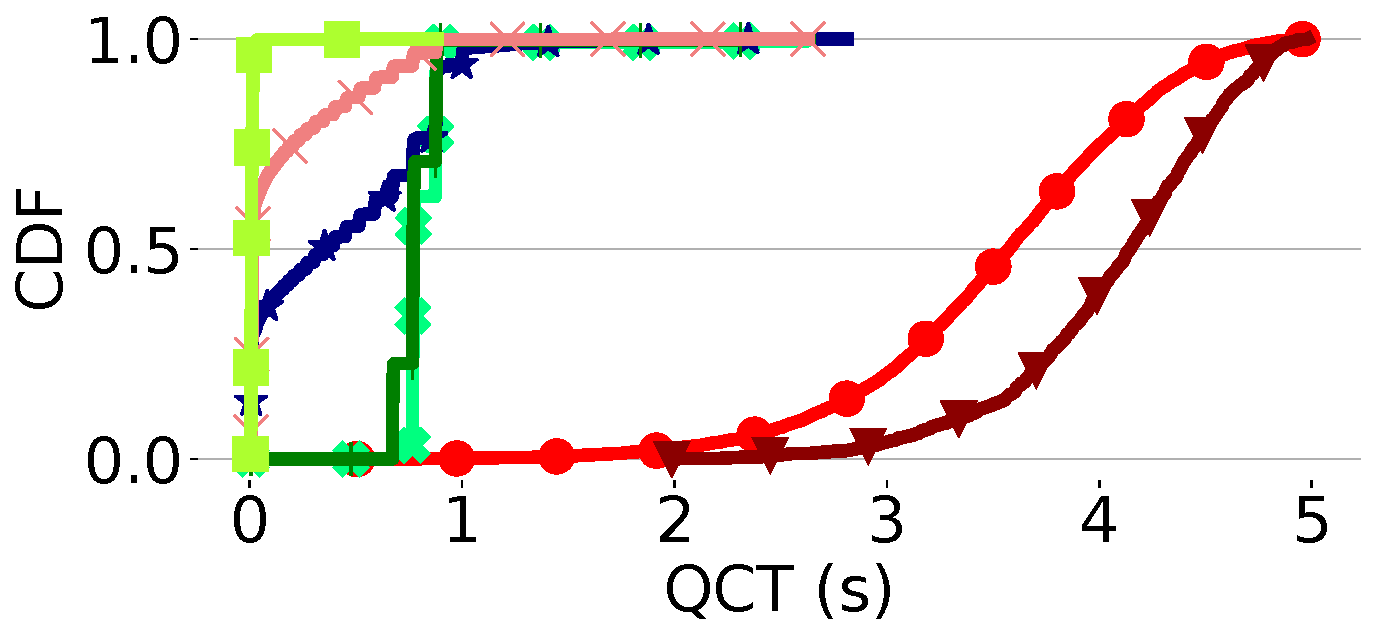
\includegraphics[width=0.98\linewidth]{figs/qps25tcpdctcpcdf.pdf}
		\caption{\small{QCT CDF}}
		\label{fig:cdf}
	\end{subfigure}
% 		\vspace{-3mm}

% 	\caption{Vertigo implicitly performs congestion control on large flows. Without congestion notification mechanisms, flows are able to automatically adjust their transmission under Vertigo.}
    \caption{\small{ Vertigo delivers low QCT with TCP, DCTCP, and Swift. 
    % CDF lines from left to right represent Vertigo+Swift, DIBS+Swift, Vertigo+TCP, Vertigo+DCTCP, DIBS+DCTCP, and DIBS+TCP, respectively. QCT lines from top to bottom represent DIBS+TCP, DIBS+DCTCP, Vertigo+TCP, Vertigo+DCTCP, ECMP+Swift, DIBS+Swift, and Vertigo+Swift.
    }}
	\label{fig:tcp}
	\vspace{-3mm}
\end{figure}

We repeat these experiments, replacing DCTCP with TCP for all schemes. 
%While explicit congestion notification (ECN) is an effective asset in most network designs, in Vertigo, we break this requirement by taking the flow size information into account. 
Our results highlight the dependence of DIBS on DCTCP. Replacing DCTCP with TCP leads up to 10$\times$ jump in DIBS' query completion times and expedites its collapse under load. In contrast, Vertigo remains efficient under TCP as well. Figure \ref{fig:tcp} shows that Vertigo+TCP outperforms other alternatives that leverage DCTCP, and performs in the close proximity of Vertigo+DCTCP.

We next replace TCP with a state-of-the-art congestion control technique, Swift \cite{swift}. Designed specifically to handle extreme and bursty datacenter workloads such as large-scale incasts, Swift is different from traditional congestion control protocols such as DCTCP and TCP along two key dimensions: (1) it leverages advanced, high-resolution hardware and software timestamps to precisely measure RTTs and rapidly react to increasing RTTs and (2) it combines window-based congestion management with packet pacing to prevent \bursts. Under extremely large incasts, with thousands of flows destined to a single host simultaneously, the number of flows exceeds the path BDP (bandwidth-delay product) and even a congestion window of one single packet is too high to prevent packet drops. Window-based congestion control algorithms such as DCTCP and TCP are fundamentally not suited for managing such extreme \bursts. To handle such cases, Swift allows the congestion window to fall below one packet, \eg \emph{cwnd}=0.5 results in sending a packet after a delay of 2RTT \cite{swift}.

Consistent with the reports from Google's datacenters that show Swift's efficiency even under extreme load (\eg 95\%) \cite{swift}, our simulations show that Swift retains low-latency under different load levels and large-scale incasts. However, our results also show that the performance of Swift can be significantly improved if it is combined with Vertigo. By selectively deflecting packets, Vertigo delays pacing and rate reduction in Swift. For example, under 25\% fixed background load combined with various levels of incast traffic raising the load up to 95\%, running Vertigo with Swift results in an order of magnitude reduction in Swift's mean QCT and zero packet loss up until the load reaches 75\%. Under 85\% and 95\% load, Vertigo+Swift drops only $2{\times}10^{-6}$\% and $2{\times}10^{-4}$\% of the packets, respectively. In comparison, with ECMP+Swift, the loss rates are 0.12\% and 0.51\%, respectively.
%We observe that the two alternatives using Swift (ECMP and Vertigo) experience \fixme{0.12}\% and \fixme{2$e^{-6}$}\% packet loss under 85\% and \fixme{0.51}\% and \fixme{2$e^{-4}$}\% packet loss under 95\% offered load, respectively. 
Under Vertigo+Swift, the drop rates are up to four orders of magnitude lower than the drop rates under Vertigo+TCP and Vertigo+DCTCP. This underscores the importance of congestion control in managing severe congestion. Similar to our previous results, DIBS is effective under low load but fails as the load increases. Figure \ref{fig:transport_qct} depicts the results.

%\textbf{Delay-based congestion control can substantially benefit from Vertigo.}
%We deploy Swift \cite{swift} a recent proposal on delay-based congestion control and repeat our incast experiments with 25\% background load using Swift as the transport protocol for ECMP, DRILL, DIBS, and Vertigo. We configure Swift with two initial congestion window settings: 10, the default value used throughout all experiments for TCP variants, and 1, to give Swift's RTT calculation more chance to converge. Figure \ref{fig:tcp} presents Swift's results with the latter setup. We observe that delay-based congestion control is highly effective in quickly recovering from microbursts by demonstrating 65\% reduction of ECMP's flow completion time tail in 85\% offered load. Nonetheless, if combined with Vertigo, Swift is able to further reduce 99-\%ile FCT and mean QCT both by 98\%. Figure \ref{fig:cdf} shows that very few incast queries experience prolonged QCTs due to large initial RTOs under Swift+Vertigo. This makes the two schemes an ultimate match for addressing high degrees of bursty traffic in datacenters. We further present the impact of initial window size on Swift's performance in figure \ref{fig:swift}. Starting the transmissions with a single packet lets Swift to quickly converge its sending rate based on congestions in the network and when combined with Vertigo, reduces the fabric packet loss to near zero.

% \begin{figure}[t]
% 	\centering
	
% 	\begin{subfigure}[t]{.49\linewidth}
% 	\centering
% 	\includegraphics[width=0.98\linewidth]{figs/fattree50qct.pdf}
% 		\caption{\small{Mean QCT}}
% 		\label{fig:fattree_qct}
% 	\end{subfigure}
% 	\begin{subfigure}[t]{.49\linewidth}
% 	\centering
% 	\includegraphics[width=0.98\linewidth]{figs/fattree50fct.pdf}
% 		\caption{\small{Mean FCT}}
% 		\label{fig:fattree_fct}
% 	\end{subfigure}
	
% 	\begin{subfigure}[t]{.49\linewidth}
% 	\centering
% 	\includegraphics[width=0.98\linewidth]{figs/fattree50p99qct.pdf}
% 		\caption{\small{p99 QCT}}
% 		\label{fig:fattree_p99qct}
% 	\end{subfigure}
% 	\begin{subfigure}[t]{.49\linewidth}
% 	\centering
% 	\includegraphics[width=0.98\linewidth]{figs/fattree50p99fct.pdf}
% 		\caption{\small{p99 FCT}}
% 		\label{fig:fattree_p99fct}
% 	\end{subfigure}
	
% 	\vspace{-3mm}
% 	\caption{\small{Fattree topologies offer more buffering capacity for deflection mechanisms to avoid dropping incast packets.}}
% 	\label{fig:fattree}
% 	\vspace{-5mm}
% \end{figure}

\begin{figure}[t]
    \begin{subfigure}[t]{.48\linewidth}
	\centering
	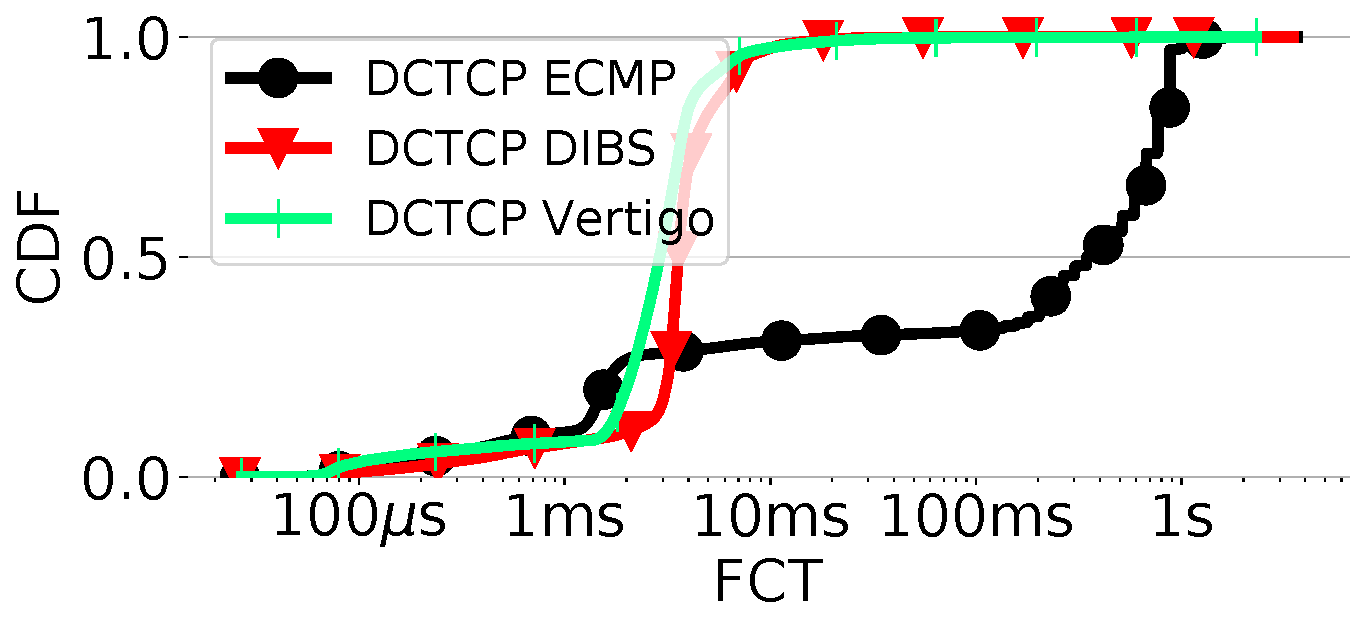
\includegraphics[width=0.49\linewidth]{figs/fattree25_35dctcpfctcdf.pdf}
	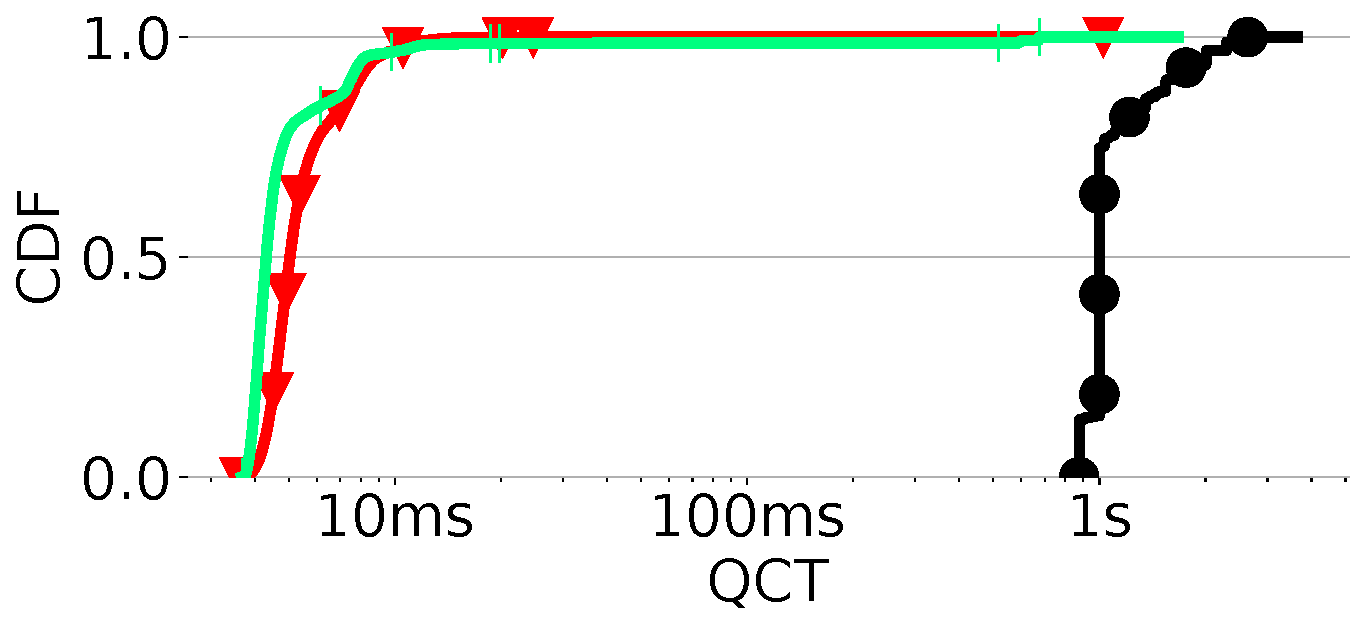
\includegraphics[width=0.49\linewidth]{figs/fattree25_35dctcpqctcdf.pdf}
		\caption{\small{25\% background + 10\% incast - DCTCP}}
		\label{fig:fattreedc35}
	\end{subfigure}
	\begin{subfigure}[t]{.48\linewidth}
	\centering
	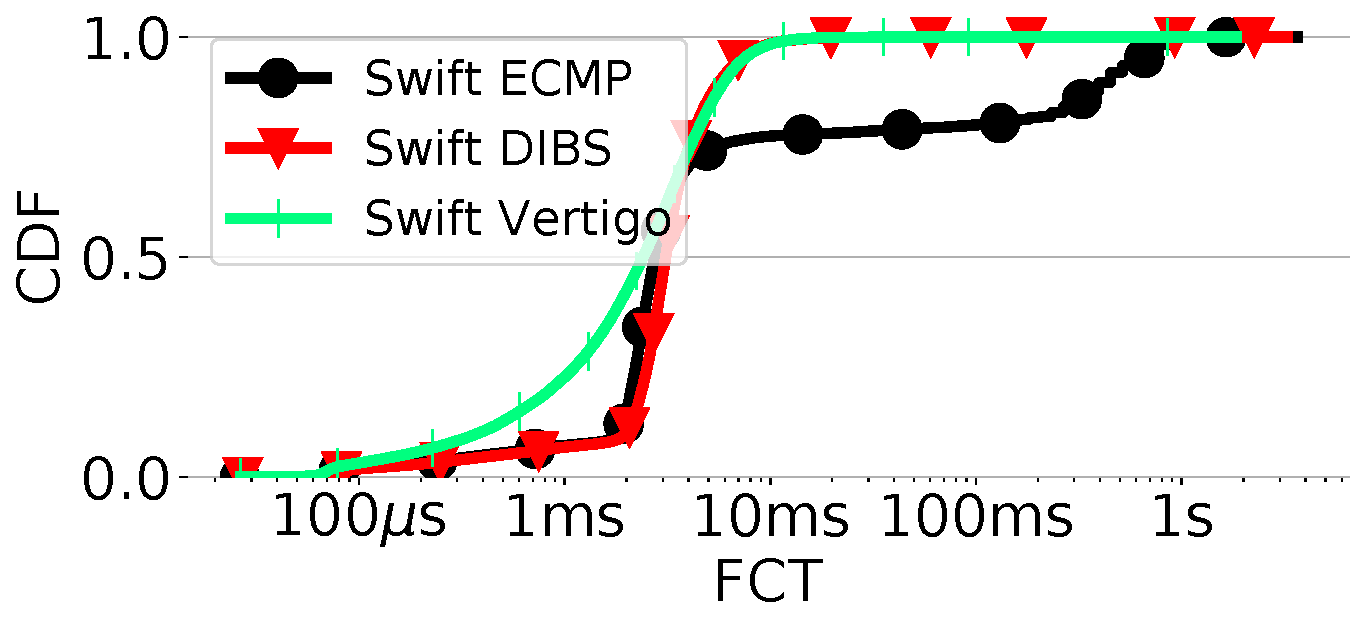
\includegraphics[width=0.49\linewidth]{figs/fattree25_35swiftfctcdf.pdf}
	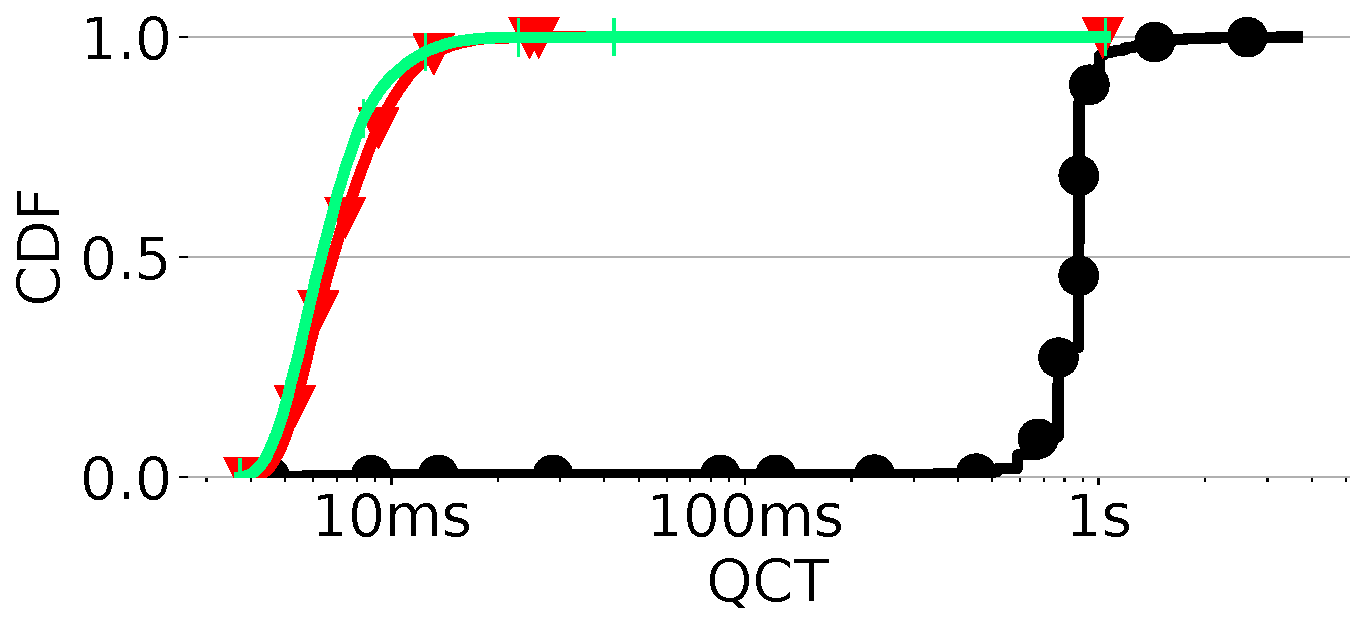
\includegraphics[width=0.49\linewidth]{figs/fattree25_35swiftqctcdf.pdf}
		\caption{\small{25\% background + 10\% incast - Swift}}
		\label{fig:fattreesw35}
	\end{subfigure}
	
	\begin{subfigure}[t]{.48\linewidth}
	\centering
	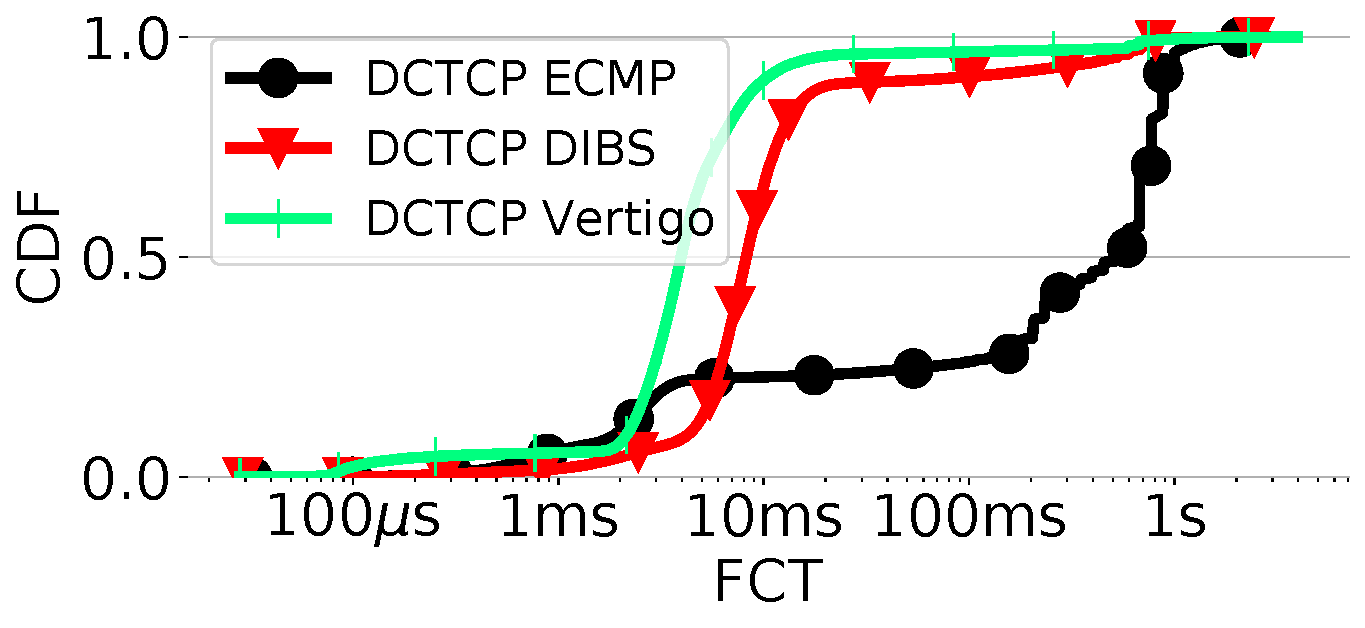
\includegraphics[width=0.49\linewidth]{figs/fattree50_25dctcpfctcdf.pdf}
	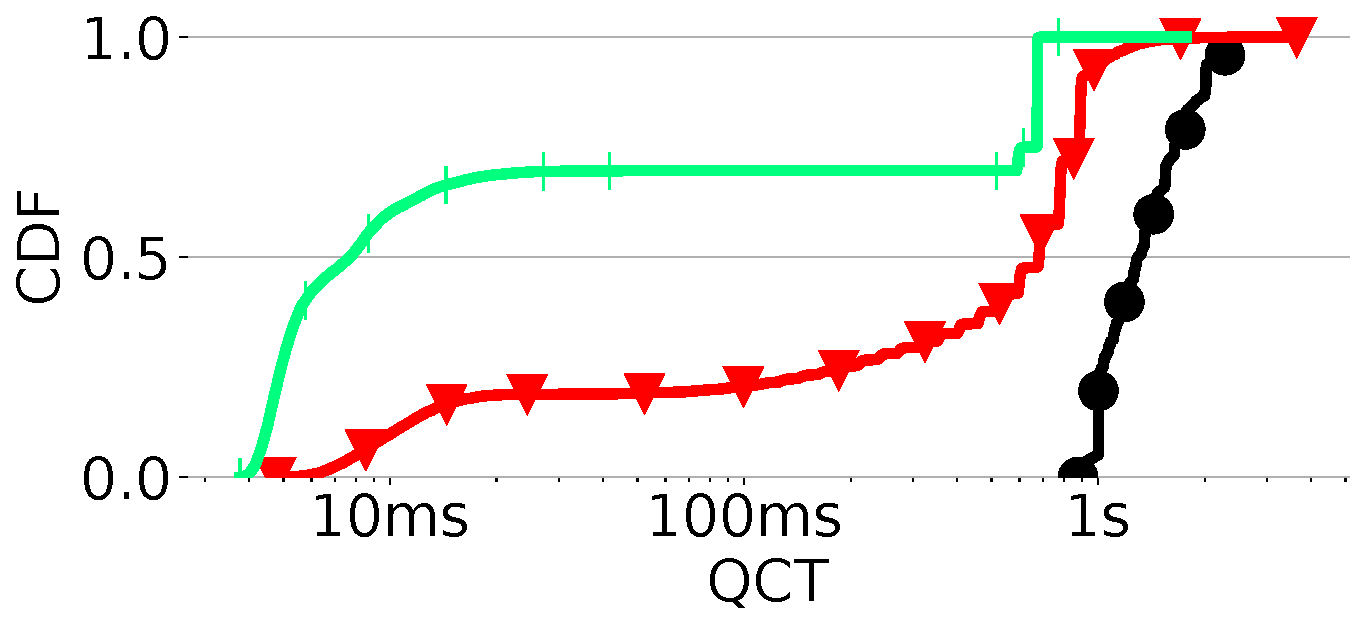
\includegraphics[width=0.49\linewidth]{figs/fattree50_25dctcpqctcdf.pdf}
		\caption{\small{50\% background + 25\% incast - DCTCP}}
		\label{fig:fattreedc75}
	\end{subfigure}
	\begin{subfigure}[t]{.48\linewidth}
	\centering
	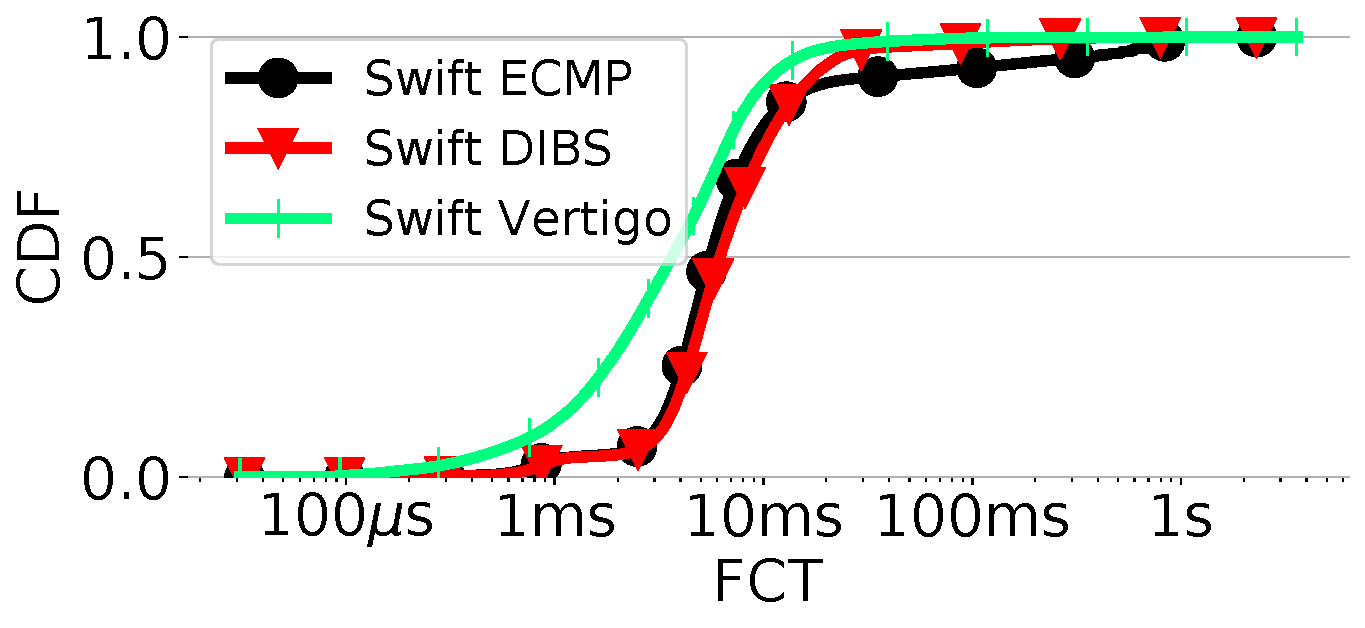
\includegraphics[width=0.49\linewidth]{figs/fattree50_25swiftfctcdf.pdf}
	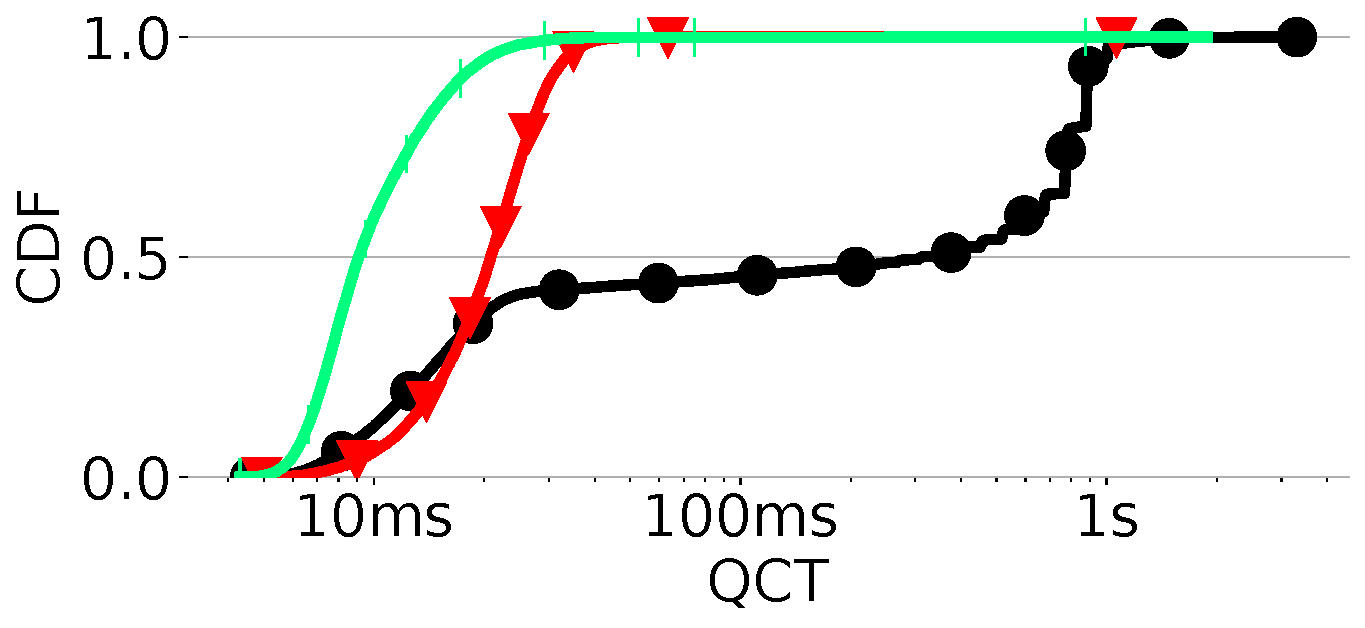
\includegraphics[width=0.49\linewidth]{figs/fattree50_25swiftqctcdf.pdf}
		\caption{\small{50\% background + 25\% incast - Swift}}
		\label{fig:fattreesw75}
	\end{subfigure}
	
    \begin{subfigure}[t]{.48\linewidth}
	\centering
	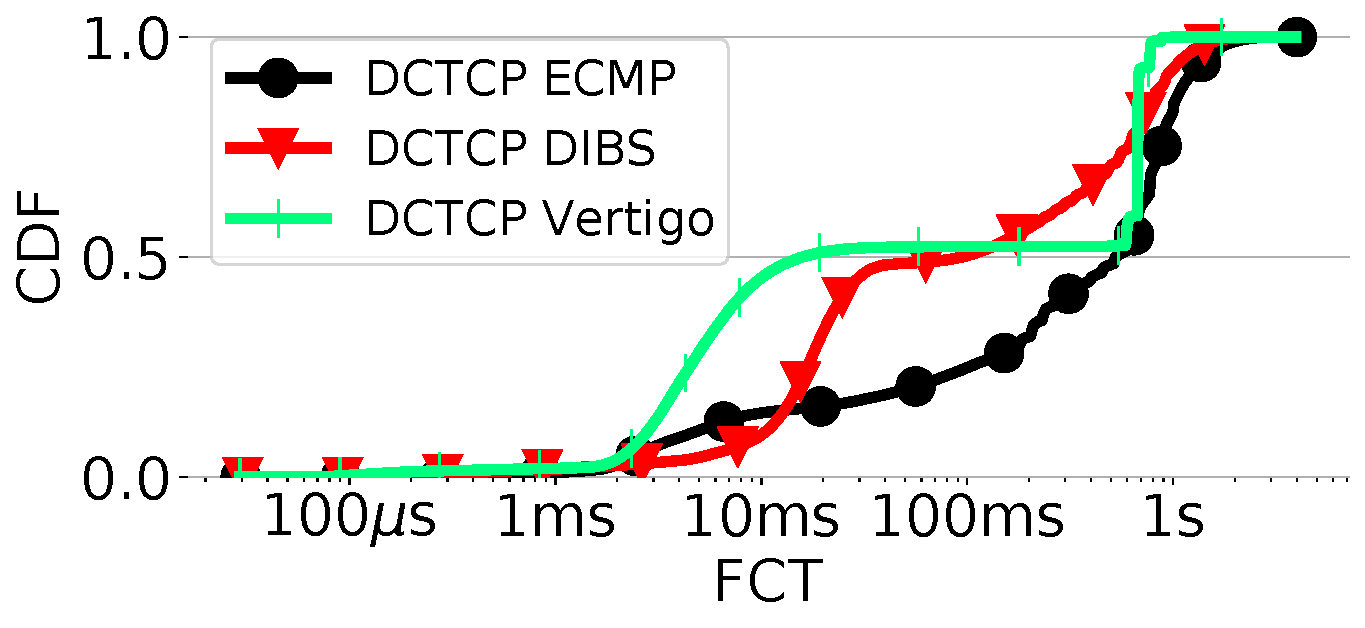
\includegraphics[width=0.49\linewidth]{figs/fattree25_85dctcpfctcdf.pdf}
	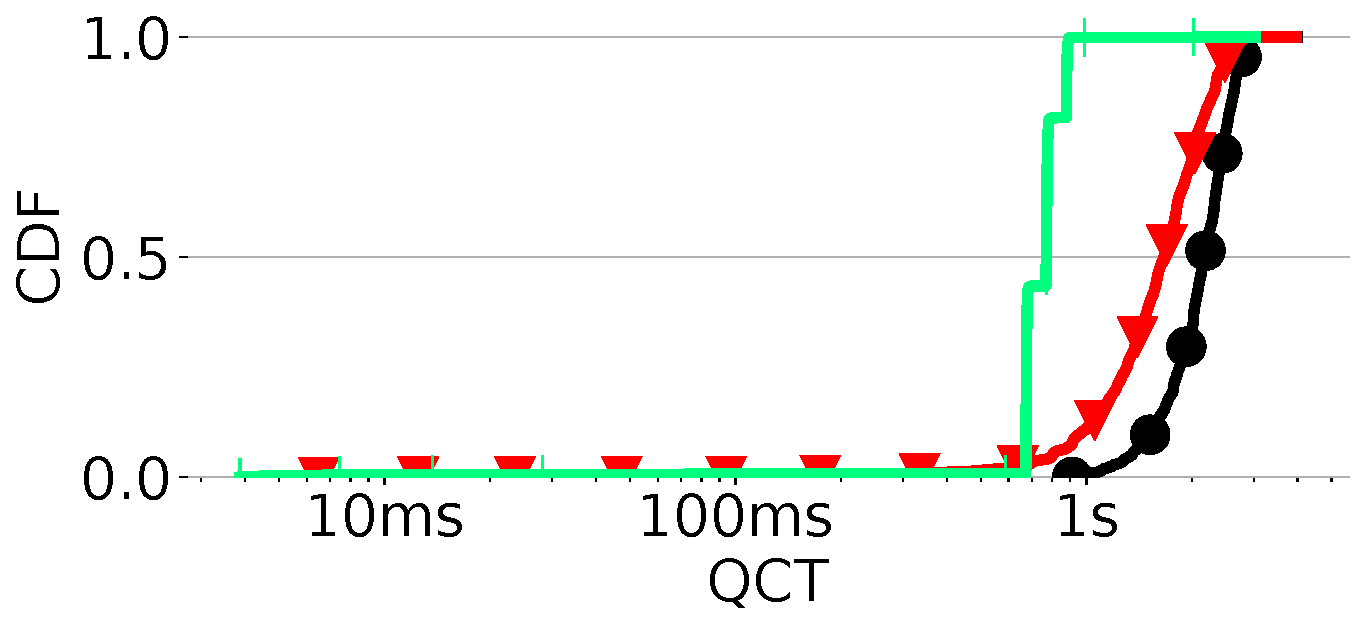
\includegraphics[width=0.49\linewidth]{figs/fattree25_85dctcpqctcdf.pdf}
		\caption{\small{25\% background + 60\% incast - DCTCP}}
		\label{fig:fattreedc85}
	\end{subfigure}
	\begin{subfigure}[t]{.48\linewidth}
	\centering
	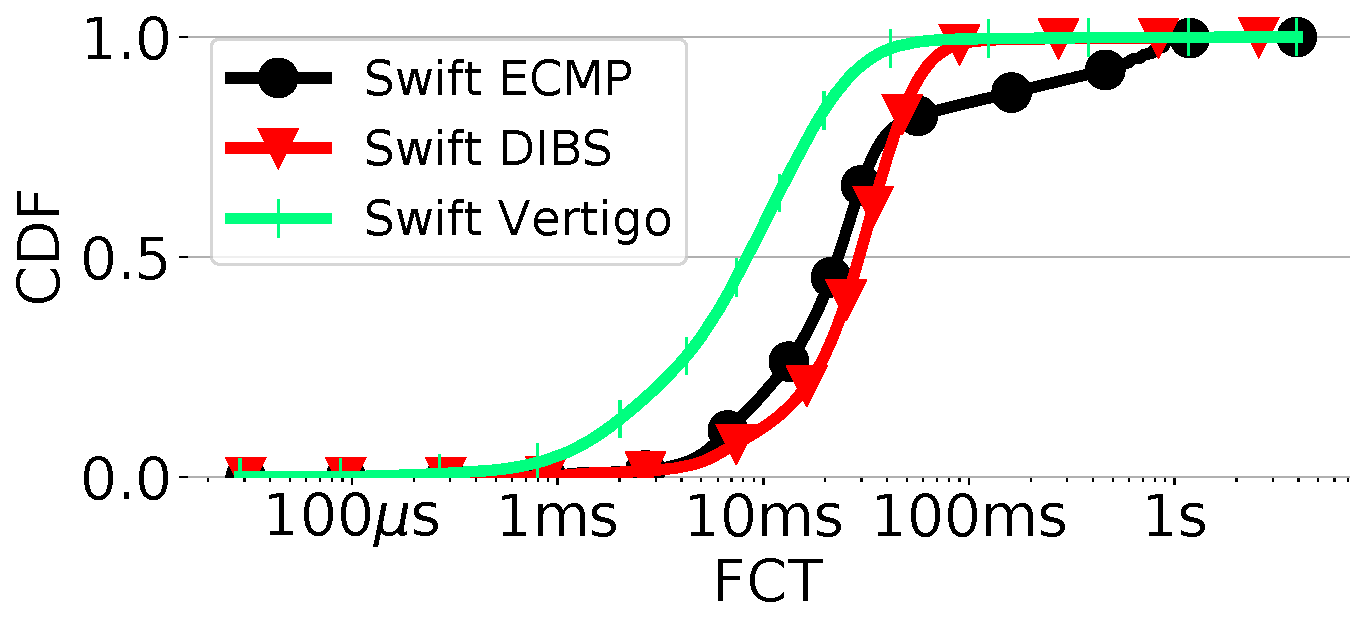
\includegraphics[width=0.49\linewidth]{figs/fattree25_85swiftfctcdf.pdf}
	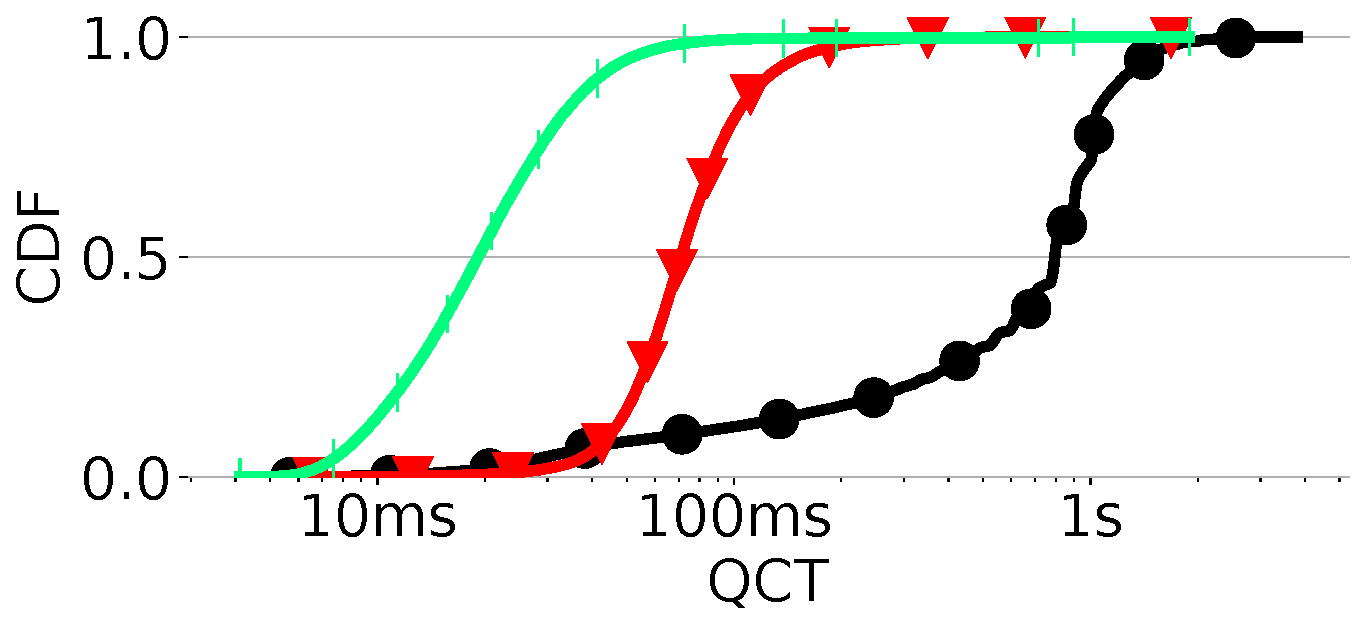
\includegraphics[width=0.49\linewidth]{figs/fattree25_85swiftqctcdf.pdf}
		\caption{\small{25\% background + 60\% incast - Swift}}
		\label{fig:fattreesw85}
	\end{subfigure}
% 	\vspace{-3mm}
	\caption{\small{Vertigo cuts the flow and query completion times of ECMP and DIBS under two congestion control schemes in a fat-tree topology.}}
	\vspace{-5mm}
	\label{fig:fattree}
\end{figure}


\textbf{Vertigo is effective in three-tiered topologies.}
To evaluate Vertigo in another common datacenter topology, we perform our simulations in a fat-tree \cite{fattree} with $k=8$ (128 servers and 80 switches) and 10Gbps links, shortening the simulation deadline to three seconds. For these experiments, we compare ECMP, DIBS, and Vertigo under three different combinations of background and incast load when using DCTCP and Swift for congestion control. Based on the results shown in Figure \ref{fig:fattree}, for a network filled with 50\% background and 25\% incast load, Vertigo can effectively reduce the QCT of ECMP under both DCTCP and Swift by 71\% and 98\%, respectively, while improving the tail QCT of random deflection by 51\% and 29\%.
This is because, with Swift, all systems experience orders of magnitude fewer drops. Therefore, even random deflection is able to considerably reduce the QCT tail of ECMP, and complete over 99\% of the incast queries within the simulation deadline. 
Table \ref{tab:completions_fattree} presents the percentage of all flows and incast queries completed before the deadline under both DCTCP and Swift. Our results indicate that, while ECMP and DRILL can heavily benefit from Swift, Vertigo is able to maintain over 98\% and 93\% flow and query completion performance, respectively, regardless of the congestion control technique. 




Additionally, with less dominant background load, we observe that the QCT and FCT of DIBS quickly degrades with the increased incast traffic load, completing only 19\% of the queries with DCTCP under 85\% load. With 85\% aggregate load consisting of 25\% background and 60\% incast (Figure \ref{fig:fattreesw85}) and DCTCP as the transport protocol, Vertigo makes use of extra 33\% buffering capacity, extra 20\% deflection destinations, and extra 4$\times$ forwarding choices in the fat-tree topology to improve the percentage of completed queries and tail QCT of random deflection by 53\% and 65\%, respectively. Finally, we observe that in all scenarios Vertigo+Swift combination offers near-0 drops akin to the two-tiered leaf-spine simulations.


\begin{table}[]
\begin{minipage}[b]{0.48\textwidth}
\resizebox{\columnwidth}{!}{%
    \begin{tabular}{|l|l|l|l|}
    \hline
    CC/System & ECMP & DIBS & Vertigo \\ \hline
    DCTCP     &  78.53\%    &    96.07\%  &   98.00\%      \\ \hline
    Swift     &   97.69\%   &  99.44\%    &   99.76\%      \\ \hline
    \end{tabular}
    }
	\subcaption{\small{\% Flow completion}}
\end{minipage}
\hfill
\begin{minipage}[b]{0.48\textwidth}
\resizebox{\columnwidth}{!}{%
	\begin{tabular}{|l|l|l|l|}
    \hline
    CC/System & ECMP & DIBS & Vertigo \\ \hline
    DCTCP     &   28.36\%   &  71.25\%    &   92.98\%      \\ \hline
    Swift     &     79.91\% & 99.06\%     &  99.57\%       \\ \hline
    \end{tabular}
    }
	\subcaption{\small{\% Query completion}}
	
\end{minipage}
\caption{\small{Flow and query completion comparison for Vertigo, DIBS, and ECMP.}}
\label{tab:completions_fattree}
\vspace{-2mm}
\end{table}

% With 50\% background load and the incast traffic load rising up to 45\%, Vertigo makes use of extra 33\% buffering capacity, extra 20\% deflection destinations, and extra 4$\times$ forwarding choices in the fat-tree topology to achieve up to 75\% lower QCT and 77\% lower FCT compared to DIBS.
% On the other hand, ECMP load-balancing demonstrates a heavy vulnerability to incast traffic and terminates at most 8\% of the queries in the simulation deadline. Our results also demonstrate that while DRILL performs similar to ECMP in a two-tiered topology, fat-tree allows for better load distribution and more timely incast query completion compared to ECMP. Nevertheless, power-of-two load-balancing is not enough to prevent long query completion time tails. Our results presented in figure \ref{fig:fattree_p99qct} show that Vertigo reduces the p99 QCT latency of DRILL by 83\% on average.

\begin{figure}[t]
	\begin{subfigure}[t]{.45\linewidth}
	\centering
	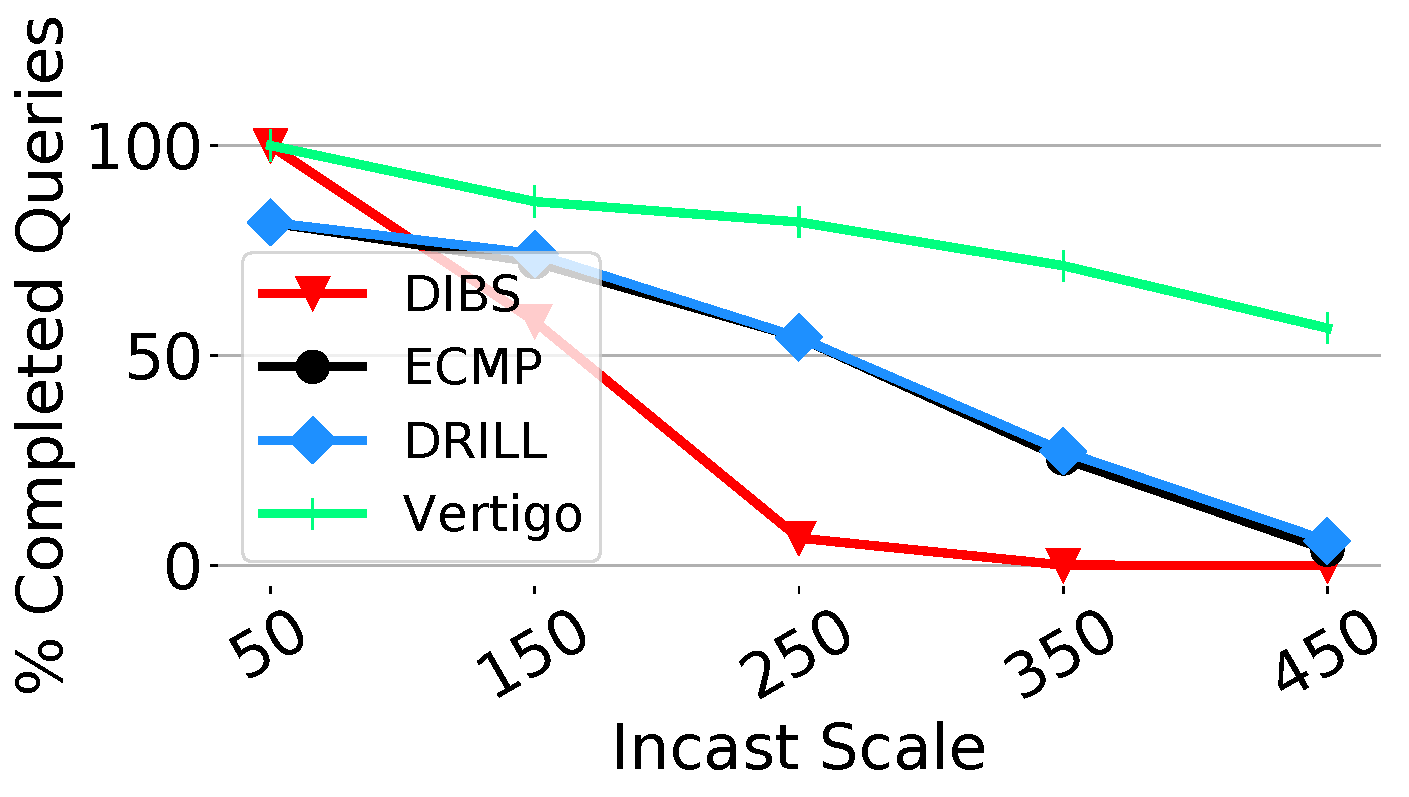
\includegraphics[width=0.98\linewidth]{figs/scale50qc.pdf}
		\caption{\small{Completed Incast Queries}}
		\label{fig:scale_qc}
	\end{subfigure}
	\begin{subfigure}[t]{.45\linewidth}
	\centering
	\includegraphics[width=0.98\linewidth]{figs/scale50qct.pdf}
		\caption{\small{Mean QCT}}
		\label{fig:scale_qct}
	\end{subfigure}
	\begin{subfigure}[t]{.45\linewidth}
	\centering
	\includegraphics[width=0.98\linewidth]{figs/scale50fctall.pdf}
		\caption{\small{Mean FCT}}
		\label{fig:scale_fctall}
	\end{subfigure}
	\begin{subfigure}[t]{.45\linewidth}
	\centering
	\includegraphics[width=0.98\linewidth]{figs/scale50fctallp99.pdf}
		\caption{\small{p99 FCT}}
		\label{fig:scale_fctbursty}
	\end{subfigure}
	\vspace{-3mm}
	\caption{\small{Vertigo completes up to 10$\times$ more queries in larger scale incast traffic patterns.}}
	\label{fig:scale}
	
	\vspace{-2mm}
\end{figure}


\textbf{Vertigo completes more queries under large-scale incast.}
Next, we gradually increase the scale of incast events from 50 to 450 while fixing the incast rate to 4000QPS and incast flow size to 40KB. With 50\% of the offered load originating from background traffic, the incast traffic elevates the overall offered load up to 95\%. Figure \ref{fig:scale} presents the results. As incast scale increases, all systems except Vertigo struggle to complete queries. That is because completing a single query requires the completion of many more individual flows. In contrast, Vertigo is able to selectively deflect, drop, and boost packets, resulting in up to 10$\times$ more completed queries compared to other alternatives. As Figure \ref{fig:scale_fctall} shows, the mean FCTs of all schemes climb with higher incast scales which is a result of more frequent drops and queueing delays for both incast and background flows. 

\textbf{Vertigo performs well even under large incast flows.}
In this experiment, affixing the background load to 50\%, we increase the overall offered load by sending larger incast flows. With 100 flows contributing to an incast event and incast rate of 4000QPS, we increase the size of the incast flows from 1K to 180KB. The results, presented in Figure \ref{fig:size}, align well with our previous findings. As the incast flow size increases, the techniques that do not take remaining flow size into account fail to categorize large flows as incast flows and forward them accordingly. Vertigo, however, is able to identify halfway completed flows and helps them finish with the combination of deflection and re-transmission boosting mechanisms. 
%We also observe that DIBS's global view of buffer occupancy allows it to prevent packet drops when the incast flow size is below 40KB. This directly results in more query completions compared to Vertigo. However, a
As the flow sizes increase, DIBS's drop rate exceeds Vertigo. With 180KB incast flows, the mean QCT of Vertigo is 68\% and 58\% lower than DIBS and DCTCP+ECMP in the rightmost datapoints, respectively.




\textbf{Burstiness is a challenge for random deflection. Vertigo performs robustly under extremely bursty traffic.}
Next, to investigate whether different degrees of burstiness can affect the overall performance of Vertigo, we fix the overall offered load to 25\%, 50\%, and 80\%, adjusting the ratio of the incast traffic by squeezing the incast interarrival times. Figure \ref{fig:burstiness80} presents the results for 80\% offered load. The QCT for all systems start to rise
% raise
as the degree of burstiness increases. Vertigo, however, delivers steadily low latency by avoiding around 15\% of packet drops and inflicting the majority of inevitable packet loss to larger flows even in the most extreme case. The results also show DIBS's limitation under heavy background load. With switch buffers partly occupied by background flow, DIBS quickly fails to handle incast queries as shown in Figure \ref{fig:burstiness80}. 
Even under a low load (25\%), we observe that Vertigo's mean QCT is 16\% lower than DIBS.
Under 25\% and 50\% load and extreme burstiness, Vertigo achieves 12\% and 55\% lower 99-\%ile FCTs compared to DIBS, respectively. 
% We repeat these experiments, varying incast scale and incast flow size to control the burstiness and observe similar trends from all systems.

\textbf{Vertigo favors short flows under less bursty workloads.}
Incasts and microbursts are the norm in today's datacenter workloads \cite{bullet, wild, social, high-resolution, jupiter}. However, we evaluate Vertigo under non-bursty traffic as well. 
Our results show that Vertigo continues to deliver a solid performance under these traffic patterns, too. 
We increase the background traffic, sampled from Facebook's cache follower, Facebook's data mining, and Google's Web search distributions, from 25\% to 90\% \cite{social, dctcp}. Cache follower is a mice-dominated workload with 50\% of the flows sending less than 24KB.
% and an average flow size of 550KB
Hence, Vertigo's SRPT forwarding combined with its micro load-balancing helps reduce the overall FCTs by up to 116\% compared to ECMP+DCTCP. 
For web search and data mining workloads that are dominated by large flows, we observe that using Vertigo leads up to a marginal 4\% increase in FCT.
%that rarely benefit from deflection mechanisms, even under higher offered loads. Therefore, 
Our results indicate that without bursty traffic and for workloads dominated by large flows, transport protocols like DCTCP are effective in recovering from infrequent drops. %Readers can find the FCT results for the three traffic distributions in appendix \ref{app:bg}.


\begin{figure}[t]
%   \centering
  \begin{minipage}[b]{0.48\textwidth}
% 	\centering
	\includegraphics[width=0.98\linewidth]{figs/flowsize50qct.pdf}
% 	\vspace{-3mm}
	\caption{\small{Vertigo maintains a high query completion rate even with large incast flows while other alternatives face frequent RTOs due to congested buffers.}}
	\label{fig:size}
  \end{minipage}
  \hfill
  \begin{minipage}[b]{0.48\textwidth}
	\centering
	\includegraphics[width=0.98\linewidth]{figs/burst80.pdf}
% 	\vspace{-3mm}
	\caption{\small{Tweaking the degree of burstiness by increasing the incast arrivals and affixing the overall offered load. Vertigo maintains low QCT performance.}}
	\label{fig:burstiness80}
  \end{minipage}
  \vspace{-2mm}
\end{figure}

\begin{figure}[t]
	\centering
		\begin{subfigure}[t]{.49\linewidth}
	\centering
	\includegraphics[width=0.98\linewidth]{figs/components50qct.pdf}
		\caption{\small{Deflection and ordering}}
		\label{fig:component}
	\end{subfigure}
		\begin{subfigure}[t]{.49\linewidth}
	\centering
	\includegraphics[width=0.98\linewidth]{figs/boosting.pdf}
		\caption{\small{Boosting}}
    	\label{fig:boost}
		
	\end{subfigure}
	\vspace{-2mm}
	\caption{\small{Each individual aspect of Vertigo's design (deflection, scheduling, ordering, and boosting) contributes to its efficiency.}}
	\label{fig:deflectionandboost}
	\vspace{-2mm}
\end{figure}

% \begin{figure}[t]
% 	\centering
	
% 	\begin{subfigure}[t]{.32\linewidth}
% 	\centering
% 	\includegraphics[width=0.98\linewidth]{figs/design_qct.pdf}
% 		\caption{Mean QCT}
% 		\label{fig:design_qct}
% 	\end{subfigure}
% 	\begin{subfigure}[t]{.32\linewidth}
% 	\centering
% 	\includegraphics[width=0.98\linewidth]{figs/design_fct.pdf}
% 		\caption{Mean FCT}
% 		\label{fig:design_fct}
% 	\end{subfigure}
% 	\begin{subfigure}[t]{.32\linewidth}
% 	\centering
% 	\includegraphics[width=0.98\linewidth]{figs/design_tput.pdf}
% 		\caption{Goodput}
% 		\label{fig:design_goodput}
% 	\end{subfigure}
% 	\caption{Comparing Vertigo with SRPT (default) and FIFO forwarding disciplines.}
% 	\label{fig:design_comparison}
% \end{figure}

% \begin{figure}[t]
% 	\begin{subfigure}[t]{.49\linewidth}
% 	\centering
% 	\includegraphics[width=0.98\linewidth]{figs/buffer85qct.pdf}
% 		\caption{Mean QCT}
% 		\label{fig:buffer_qct}
% 	\end{subfigure}
% 	\begin{subfigure}[t]{.49\linewidth}
% 	\centering
% 	\includegraphics[width=0.98\linewidth]{figs/buffer85rt.pdf}
% 		\caption{Mean FCT}
% 		\label{fig:size_fct}
% 	\end{subfigure}
% 	\caption{Impact of increasing the buffer size on incast query completions and flow completion times.}
% 	\label{fig:buffer}
% \end{figure}


\subsection{Vertigo Design Deep-dive}
\label{sec:component}
\textbf{Component Analysis.}
Vertigo relies on three main components responsible for (1) deflecting packets that arrive at a full buffer (instead of simply dropping them), (2) SRPT scheduling in the network core (as opposed to FIFO), and (3) retrieving the correct ordering of out-of-order packets before sending them to higher layers.
%packets based on their remaining flow size  as a means to revive microburst flows via deflection and avoid HoL blocking via forwarding, and (3) buffering and ordering out-of-order packets stemming from packet deflection and scheduling at the destination. 
We quantify the impact of each of these components on the overall superior performance of Vertigo in Figure \ref{fig:component}.
The key contribution of packet deflection is avoiding drops, and consequently, RTOs.
% when the load is high), without deflection, FCT increases by Y% because of Z.
We observe that in the lowest load, without deflection, QCT increases by a factor of 13$\times$ as the packet loss raises by 6$\times$. Disabling the scheduler, however, has an even more notable effect as it reduces Vertigo's performance to that of random deflection alternatives. For example, in high loads, without scheduling, Vertigo suffers from up to 110\% increase in mean QCT. We also repeat the experiments with Vertigo without its ordering layer. While packet re-ordering has minimal impact on QCT, it increases the overall FCT by up to 9\% and reduces the overall goodput by 7\% as reordering causes the larger flows' windows to shrink.

% Boosting the re-transmitted packets is another critical player in the overall performance of Vertigo. We start by disabling the boosting mechanism (the leftmost columns in Figure \ref{fig:boost}). Then, starting from 2$\times$, we try various power of two boosting factors up to 8$\times$. We observe that boosting is essential in completing flows that experience packet drops; Vertigo's query completion rate drops by 65\% without boosting. 
% However, boosting packets more aggressively (boosting factors above 2$\times$) does not cause a noticeable improvement, since the majority of re-transmitted packets successfully reach their destination in the second attempt with the boosting factor of 2$\times$.

\textbf{Re-transmission boosting is key in completing incast queries.}
Boosting the re-transmitted packets is another critical player in the overall performance of Vertigo.
We start by disabling the boosting mechanism (the leftmost columns in Figure \ref{fig:boost}). Then, starting from 2$\times$ (the default factor for reducing the packet RFS values for every re-transmission), we try various powers of two boosting factors up to 8$\times$. We observe that boosting is essential in completing flows that experience packet drops; Vertigo's query completion rate drops by 65\% without boosting. 
However, boosting packets more aggressively (boosting factors above 2$\times$) does not cause a noticeable improvement, since the majority of re-transmitted packets successfully reach their destination in the second attempt with the boosting factor of 2$\times$.


\begin{figure}[t]
	\centering
		\begin{subfigure}[t]{.49\linewidth}
    	\centering
		\includegraphics[width=0.99\linewidth]{figs/powerofx25.pdf}
    	\caption{\small{QCT under two-tiered LS}}
    	\label{fig:lb-qct-ls}
	\end{subfigure}
	\hfill{}
	\begin{subfigure}[t]{.49\linewidth}
    	\centering
		\includegraphics[width=0.99\linewidth]{figs/powerofxdrops25.pdf}
    	\caption{\small{Drops under two-tiered LS}}
    	\label{fig:lbdrops-ls}
	\end{subfigure}
	\begin{subfigure}[t]{.49\linewidth}
    	\centering
		\includegraphics[width=0.99\linewidth]{figs/powerofx25fattree.pdf}
    	\caption{\small{QCT under fat-tree}}
	\end{subfigure}
	\hfill{}
	\begin{subfigure}[t]{.49\linewidth}
    	\centering
		\includegraphics[width=0.99\linewidth]{figs/powerofxdrops25fattree.pdf}
    	\caption{\small{Drops under fat-tree}}
    	\label{fig:lbdrops}
	\end{subfigure}
	\caption{\small{
    Evaluating random and power-of-two techniques for forwarding and deflection in Vertigo. The power-of-two-choices paradigm reduces packet drops and QCTs under low and medium loads.
	}}
	\label{fig:vertigo-lb}
	\vspace{-3mm}
\end{figure}

\textbf{Comparing random and power-of-2 load-balancing on deflection and forwarding.}
Vertigo uses the power of two choices scheme for its forwarding and deflection decisions. To measure the impact of this load balancing paradigm on Vertigo's performance, we preform four sets of incast simulations with 50\% background load and various incast QPS rates, trying out random and power of two choices load-balancing for forwarding (~$\widehat{}$~1 FW and ~$\widehat{}$~2 FW, respectively) and deflection (~$\widehat{}$~1 DEF and ~$\widehat{}$~2 DEF, respectively). We present our results in Figure \ref{fig:vertigo-lb}. We observe that randomly choosing a destination for deflected packets increases the chance of packet drops by up to 47\%, severely damaging the query completions. The gap, however, begins to fade as the offered load increases. This is because, in higher network loads, the probability of finding free buffer space is significantly reduced. 



\textbf{Alternative marking disciplines.}
Flow size information is a reliable indicator of flow persistence and can be used to achieve near-optimal scheduling performance. However, if the flow size information is not available, Vertigo resorts to \textit{flow aging} instead.
Under this scheduling discipline, also known as \textit{Least Attained Service (LAS)}, flows are initially marked with 0, regardless of their size. The consecutive packets carry a counter that shows the total number of packets sent by their flow or flow's age in packet units. We adapted the host components to implement LAS and repeated our previous simulations. Table \ref{tab:las} shows the results.
LAS takes a few transmissions to differentiate between flows. Consequently, its initial decisions are suboptimal compared to SRPT.  
%, aggravating the incast blow on query completion times. 
We observed up to 30\% difference in the mean QCTs under SRPT and LAS with different workloads. However, Vertigo+LAS still outperforms other baselines such as ECMP and DIBS by 52\% and 70\% under 85\% offered load, respectively.

\textbf{Vertigo's re-ordering timeout setting has a bounded effect on flow completion times.}
Finally, to demonstrate the effectiveness of Vertigo's ordering extension in detecting and resolving packet re-ordering, we repeat our incast simulations, raising the ordering timeout ($\tau$) from 120$\mu s$ up to 1.08ms. The results presented in Figure \ref{fig:ord} suggest that setting the timeout to the maximum delay a packet might experience in the network without being deflected, as described in \S \ref{sec:ordering}, is indeed a good estimate as the majority of out of order packets are not deflected. We observe that the latency penalty of improper timeout setting does not exceed a few milliseconds (5ms in our simulations) in abundance of incast flows in an extremely congested network.

% \textbf{Impact of SRPT forwarding.}
% To avoid head-of-the line blocking, Vertigo uses per-packet SRPT buffers in the fabric to quickly identify drop and deflection candidates. Alternatively, one would suggest keeping separate data structures for packet scheduling and deflection to maintain the traditional FIFO ordering in the switch buffers. Therefore, we implement a variant of Vertigo that uses the remaining flow size information only for packet drops and deflection, while resorting to the arrival ordering of the packets for forwarding them. We compare this variant with the original Vertigo and present the findings in Figure \ref{fig:design_comparison}. We observe that the difference between FIFO packet scheduling and SRPT scheduling exhibits itself when the traffic distribution is changed from 25\% background + 70\% incast to 75\% background + 20\% incast. While All three scenarios offer an equal load to the datacenter network core, the latter scenario consists of more elephant flows. That makes a case for avoiding head-of-the-line blocking via an SRPT packet scheduler. Alternatively, FIFO forwarding eliminates the main source of packet re-ordering in the network, achieves less than 1\% improvement in both FCT and QCT compared to our default variant when the background traffic ratio is low, and improves the overall goodput by letting more throughput-intensive flows through the buffers.


% \begin{figure}[t]
% 	\includegraphics[width=0.60\linewidth]{figs/timeouts.pdf}
% 	\caption{Setting the ordering timeout to high values has but a negligible impact on flow completion times.}
% 	\label{fig:ord}
% \end{figure}

% \subsection{Parameter-sensitivity runs}
% \label{sec:parameter}
% \textbf{Vertigo performs well even on shallow buffers.}
% Spare buffer capacity is the key for the deflection-based mechanisms to effectively revive from packet drops. In this experiment, we run a mixed workload comprising of 75\% background and 10\% incast flows while increasing the buffer capacity of the network switches from 50KB ($\sim$ 1/6 of commodity hardware) to 800KB ($\sim 3 \times$  of commodity hardware). The results are presented in Figure \ref{fig:buffer}. When using shallow buffers, RTOs dominate the response times, even for deflection-based mechanisms, however, with more buffer space, the number of packet drops is reduced substantially, and all systems begin to complete incast flows, and consequently incast queries, faster. The improvement in the QCT and flow completion times of deflection-based mechanisms continue to the point where all incasts are blunted by the excessive buffering in the switches at 500KB. The results also show that as DIBS finds more buffering space, its performance reaches Vertigo. That is because, all incast packets now get a second chance in an empty buffer and all the RTOs are avoided by both techniques.

\begin{figure}[t]
\centering
\begin{minipage}[b]{0.48\textwidth}
    \resizebox{\columnwidth}{!} &  \multicolumn{1}{|c|}{0.98}                          & \multicolumn{1}{|c|}{0.02}  &  \multicolumn{1}{c|}{0.06}   &  \multicolumn{1}{|c}{0.14}                       \\
    \multicolumn{1}{c|}{65\%}         &   \multicolumn{1}{|c|}{1.08}                         &   \multicolumn{1}{|c|}{0.74} & \multicolumn{1}{c|}{0.32}   &   \multicolumn{1}{|c}{0.40}                      \\
    \multicolumn{1}{c|}{75\%}         &    \multicolumn{1}{|c|}{1.22}                        &  \multicolumn{1}{|c|}{1.81} & \multicolumn{1}{c|}{0.56}    & \multicolumn{1}{|c}{0.59}   \\
    \multicolumn{1}{c|}{85\%}         &     \multicolumn{1}{|c|}{1.61}                       &   \multicolumn{1}{|c|}{2.56} & \multicolumn{1}{c|}{0.67}   &   \multicolumn{1}{|c}{0.77}                      \\
    \multicolumn{1}{c|}{95\%}         &     \multicolumn{1}{|c|}{2.34}                       &  \multicolumn{1}{|c|}{3.12} & \multicolumn{1}{c|}{0.72}   &    \multicolumn{1}{|c}{0.94}                     \\
    \end{tabular}
    }
    \vspace{2mm}
    \captionof{table}{\small{Flow aging is less effective than SRPT, but outperforms other baselines.}}
    \vspace{-2mm}
    \label{tab:las}
\end{minipage}
\hspace{3pt}
\begin{minipage}[b]{0.48\textwidth}
	\includegraphics[width=1\linewidth]{figs/timeouts.pdf}
	\vspace{-5mm}
	\captionof{figure}{\small{Ordering timeout configuration has a negligible impact on flow completion times.}}
	\label{fig:ord}
\end{minipage}
\vspace{-2mm}
\end{figure}


\subsection{End-host and Switch Implementation}
\label{sec:vertigo-testbed}
We deploy Vertigo's host components, on a physical testbed consisting of two Cloudlab \cite{cloudlab} machines, featuring two Intel Xeon E5-2640v4 processors, 64GB of memory, and 25Gbps Mellanox ConnectX-4 network interface cards. We build
a packet generator tool on top of Vertigo's userspace network stack and measure
the RTTs and throughput of a single-threaded TCP server with the marking and ordering components enabled/disabled.
To ensure minimal packet processing overheads in Vertigo, we use DPDK cuckoo filters for flow identification at both the marking and ordering components. For the packet header hash, we use pre-allocated pools of fast hash tables and modify the existing ring buffer implementations in DPDK to store out-of-order packets.
Our results indicate that the two extra hash table look-ups performed by Vertigo's marking component require an additional 300ns processing time. However, the throughput results demonstrate <0.1\% difference when Vertigo's marking component is enabled.

Recent endeavors on designing hardware-based priority queues enable programmable scheduling in data-plane at line-rate \cite{pifo, pieo, calendar}. To implement a Vertigo switch, two mechanisms must be added to existing implementations of the priority queue: 1. \textit{The ability to extract items from the tail of the priority list.} In Vertigo, packets that arrive at a full buffer still might get a buffering space if their remaining flow size is smaller than that of a buffered packet. 
To this end, we extend PIEO's abstractions \cite{pieo} to support packet extraction from the tail of the queue. Similar to other functionalities supported by PIEO, the packet extraction process is executed in 4 cycles.
%Thus, PIFO's priority encoder can be extended to identify packet ranks in reverse order.
2. \textit{The ability to change the output port for a packet when a buffer is full.} With \textit{negative mirroring} functionality already available in PISA switches \cite{opentofino} and fast SRAM access in re-configurable switches \cite{pieo}, Vertigo can perform deflection in just a few clock cycles. To that end, we extended the functionality of PIEO \cite{pieo} to find that deflection, a special case of enqueue operation requires one additional dequeue, adding 4 extra cycles. Since packet drops remain scant compared to the overall flowing traffic, the amortized cost of insertion remains unchanged. We leave the full hardware implementation of a Vertigo switch and testbed evaluations using this switch to future work.

\section{Conclusion}
%The burstiness of datacenters' traffic and their frequently low utilization suggest that deflection routing may prevent the destructive impact of packet loss. 
Short-lived congestion events that cause excessive packet loss remain a major challenge in datacenter networks. Frequently low utilization is datacenters suggests that temporarily deflecting burst packets to switches with spare capacity may prevent packet loss.
In this study we identify the main issues that stem from random packet deflection and address them by introducing Vertigo, a hybrid design that incorporate end-hosts' knowledge of the workload and the network's immediate reaction capacity to selectively deflect packets that arrive at full buffers to the
% empty 
% \sepehr{less congested}
neighboring switches. Our simulation results demonstrate that Vertigo provides up to 3.3$\times$ lower mean incast query completion times and 3$\times$ lower 99-\%ile flow completion times compared to DCTCP+ECMP while improving the mean QCT by 18$\times$ when combined with Swift. % to widely deployed in-network alternatives.